\documentclass[a4paper]{article}
\usepackage{parskip}
\usepackage{lipsum}

\def\nterm {Spring}
\def\nyear {2025}
\def\ncourse {Mathematical Studies Analysis}

\makeatletter
\ifx \nauthor\undefined
  \def\nauthor{Runqiu Ye}
\else
\fi

\author{Notes taken by \nauthor\vspace{5pt}\\ 
Carnegie Mellon University}
\date{\nterm\ \nyear}

\usepackage{alltt}
\usepackage{amsfonts}
\usepackage{amsmath}
\usepackage{amssymb}
\usepackage{amsthm}
\usepackage{booktabs}
\usepackage{caption}
\usepackage{enumitem}
\usepackage{fancyhdr}
\usepackage{graphicx}
\usepackage{mathdots}
\usepackage{mathtools}
\usepackage{microtype}
\usepackage{multirow}
\usepackage{pdflscape}
\usepackage{pgfplots}
\usepackage{siunitx}
\usepackage{slashed}
\usepackage{tabularx}
\usepackage{tikz}
\usepackage{tkz-euclide}
\usepackage[normalem]{ulem}
\usepackage[all]{xy}
\usepackage{imakeidx}
\usepackage[includehead,includefoot, heightrounded,  left=1.0in, top=1.6cm, bottom=2.4cm, right=1.0in]{geometry}
\usepackage{mathrsfs}

\makeindex[intoc, title=Index]
\indexsetup{othercode={\lhead{\emph{Index}}}}

\ifx \nextra \undefined
  \usepackage[pdftex,
    hidelinks,
    pdfauthor={Dexter Chua},
    pdfsubject={\ncourse},
    pdftitle={\ncourse},
  pdfkeywords={Cambridge Mathematics Maths Math \nterm\ \nyear\ \ncourse}]{hyperref}
  \title{\ncourse}
\else
  \usepackage[pdftex,
    hidelinks,
    pdfauthor={Dexter Chua},
    pdfsubject={Cambridge Maths Notes: \ncourse\ (\nextra)},
    pdftitle={\ncourse\ (\nextra)},
  pdfkeywords={Cambridge Mathematics Maths Math \nterm\ \nyear\ \ncourse\ \nextra}]{hyperref}

  \title{\ncourse \\ {\Large \nextra}}
  \renewcommand\printindex{}
\fi

\pgfplotsset{compat=1.12}

\pagestyle{fancyplain}
\ifx \ncoursehead \undefined
\def\ncoursehead{\ncourse}
\fi

\lhead{\emph{\nouppercase{\leftmark}}}
\ifx \nextra \undefined
  \rhead{
    \ifnum\thepage=1
    \else
      \ncoursehead
    \fi}
\else
  \rhead{
    \ifnum\thepage=1
    \else
      \ncoursehead \ (\nextra)
    \fi}
\fi
\usetikzlibrary{arrows.meta}
\usetikzlibrary{decorations.markings}
\usetikzlibrary{decorations.pathmorphing}
\usetikzlibrary{positioning}
\usetikzlibrary{fadings}
\usetikzlibrary{intersections}
\usetikzlibrary{cd}

\newcommand*{\Cdot}{{\raisebox{-0.25ex}{\scalebox{1.5}{$\cdot$}}}}
\newcommand {\pd}[2][ ]{
  \ifx #1 { }
    \frac{\partial}{\partial #2}
  \else
    \frac{\partial^{#1}}{\partial #2^{#1}}
  \fi
}
\ifx \nhtml \undefined
\else
  \renewcommand\printindex{}
  \DisableLigatures[f]{family = *}
  \let\Contentsline\contentsline
  \renewcommand\contentsline[3]{\Contentsline{#1}{#2}{}}
  \renewcommand{\@dotsep}{10000}
  \newlength\currentparindent
  \setlength\currentparindent\parindent

  \newcommand\@minipagerestore{\setlength{\parindent}{\currentparindent}}
  \usepackage[active,tightpage,pdftex]{preview}
  \renewcommand{\PreviewBorder}{0.1cm}

  \newenvironment{stretchpage}%
  {\begin{preview}\begin{minipage}{\hsize}}%
    {\end{minipage}\end{preview}}
  \AtBeginDocument{\begin{stretchpage}}
  \AtEndDocument{\end{stretchpage}}

  \newcommand{\@@newpage}{\end{stretchpage}\begin{stretchpage}}

  \let\@real@section\section
  \renewcommand{\section}{\@@newpage\@real@section}
  \let\@real@subsection\subsection
  \renewcommand{\subsection}{\@ifstar{\@real@subsection*}{\@@newpage\@real@subsection}}
\fi
\ifx \ntrim \undefined
\else
  \usepackage{geometry}
  \geometry{
    papersize={379pt, 699pt},
    textwidth=345pt,
    textheight=596pt,
    left=17pt,
    top=54pt,
    right=17pt
  }
\fi

\ifx \nisofficial \undefined
\let\@real@maketitle\maketitle
\renewcommand{\maketitle}{\@real@maketitle}
\else
\fi

% Theorems
\theoremstyle{definition}
\newtheorem*{aim}{Aim}
\newtheorem*{axiom}{Axiom}
\newtheorem*{claim}{Claim}
\newtheorem*{cor}{Corollary}
\newtheorem*{conjecture}{Conjecture}
\newtheorem*{defi}{Definition}
\newtheorem*{eg}{Example}
\newtheorem*{ex}{Exercise}
\newtheorem*{fact}{Fact}
\newtheorem*{law}{Law}
\newtheorem*{lemma}{Lemma}
\newtheorem*{notation}{Notation}
\newtheorem*{prop}{Proposition}
\newtheorem*{question}{Question}
\newtheorem*{rrule}{Rule}
\newtheorem*{thm}{Theorem}
\newtheorem*{assumption}{Assumption}

\newtheorem*{remark}{Remark}
\newtheorem*{warning}{Warning}
\newtheorem*{exercise}{Exercise}

\newtheorem{nthm}{Theorem}[section]
\newtheorem{nlemma}[nthm]{Lemma}
\newtheorem{nprop}[nthm]{Proposition}
\newtheorem{ncor}[nthm]{Corollary}


\renewcommand{\labelitemi}{--}
\renewcommand{\labelitemii}{$\circ$}
% \renewcommand{\labelenumi}{(\roman{*})}

\let\stdsection\section
\renewcommand\section{\newpage\stdsection}

\newcommand\qedsym{\hfill\ensuremath{\square}}
% Strike through
\def\st{\bgroup \ULdepth=-.55ex \ULset}



%%%%%%%%%%%%%%%%%%%%%%%%%
%%%%% Maths Symbols %%%%%
%%%%%%%%%%%%%%%%%%%%%%%%%
\newcommand{\cupinfn}{\bigcup_{n=0}^\infty}
\newcommand{\capinfn}{\bigcap_{n=0}^\infty}
\newcommand{\suminfn}{\sum_{n=0}^\infty}
\newcommand{\seqinfn}[1]{\left\{ #1 \right\}_{n=0}^\infty}
\newcommand{\cupinfk}{\bigcup_{k=0}^\infty}
\newcommand{\capinfk}{\bigcap_{k=0}^\infty}
\newcommand{\suminfk}{\sum_{k=0}^\infty}
\newcommand{\seqinfk}[1]{\left\{ #1 \right\}_{k=0}^\infty}
\newcommand{\cupinfm}{\bigcup_{m=0}^\infty}
\newcommand{\capinfm}{\bigcap_{m=0}^\infty}
\newcommand{\suminfm}{\sum_{m=0}^\infty}
\newcommand{\seqinfm}[1]{\left\{ #1 \right\}_{m=0}^\infty}

\newcommand{\cupn}{\bigcup_{n=0}}
\newcommand{\capn}{\bigcap_{n=0}}
\newcommand{\sumn}{\sum_{n=0}}
\newcommand{\seqn}[1]{\left\{ #1 \right\}_{n=0}}
\newcommand{\cupk}{\bigcup_{k=0}}
\newcommand{\capk}{\bigcap_{k=0}}
\newcommand{\sumk}{\sum_{k=0}}
\newcommand{\seqk}[1]{\left\{ #1 \right\}_{k=0}}
\newcommand{\cupm}{\bigcup_{m=0}}
\newcommand{\capm}{\bigcap_{m=0}}
\newcommand{\summ}{\sum_{m=0}}
\newcommand{\seqm}[1]{\left\{ #1 \right\}_{m=0}}

% Analysis
\newcommand{\om}{\mu^*}
\newcommand{\fs}{F_\sigma}
\newcommand{\gd}{G_\delta}
\newcommand{\cale}{\mathcal{E}}
\newcommand{\calf}{\mathcal{F}}
\newcommand{\mf}{\mathfrak{M}}
\newcommand{\nf}{\mathfrak{N}}
\newcommand{\bfk}{\mathfrak{B}}
\def\L{\mathcal{L}}
\def\H{\mathcal{H}}
\renewcommand{\P}{\mathcal{P}}
\DeclareMathOperator{\Rec}{Rec}
\DeclareMathOperator{\Cube}{Cube}
\DeclareMathOperator{\RCube}{RCube}
\newcommand{\RCuber}{\RCube_r}
\DeclareMathOperator{\Reco}{Rec^{\circ}}
\DeclareMathOperator{\Cubeo}{Cube^{\circ}}
\DeclareMathOperator{\RCubeo}{RCube^{\circ}}
\newcommand{\RCubeor}{\RCube^{\circ}_r}

% Matrix groups
\newcommand{\GL}{\mathrm{GL}}
\newcommand{\Or}{\mathrm{O}}
\newcommand{\PGL}{\mathrm{PGL}}
\newcommand{\PSL}{\mathrm{PSL}}
\newcommand{\PSO}{\mathrm{PSO}}
\newcommand{\PSU}{\mathrm{PSU}}
\newcommand{\SL}{\mathrm{SL}}
\newcommand{\SO}{\mathrm{SO}}
\newcommand{\Spin}{\mathrm{Spin}}
\newcommand{\Sp}{\mathrm{Sp}}
\newcommand{\SU}{\mathrm{SU}}
\newcommand{\U}{\mathrm{U}}
\newcommand{\Mat}{\mathrm{Mat}}

% Matrix algebras
\newcommand{\gl}{\mathfrak{gl}}
\newcommand{\ort}{\mathfrak{o}}
\newcommand{\so}{\mathfrak{so}}
\newcommand{\su}{\mathfrak{su}}
\newcommand{\uu}{\mathfrak{u}}
\renewcommand{\sl}{\mathfrak{sl}}

% Special sets
\newcommand{\C}{\mathbb{C}}
\newcommand{\CP}{\mathbb{CP}}
\newcommand{\GG}{\mathbb{G}}
\newcommand{\N}{\mathbb{N}}
\newcommand{\Q}{\mathbb{Q}}
\newcommand{\R}{\mathbb{R}}
\newcommand{\RP}{\mathbb{RP}}
\newcommand{\T}{\mathbb{T}}
\newcommand{\Z}{\mathbb{Z}}
% \renewcommand{\H}{\mathbb{H}}

% Brackets
\renewcommand{\bar}[1]{\overline{#1}}
\renewcommand{\tilde}[1]{\widetilde{#1}}
\renewcommand{\hat}[1]{\widehat{#1}}
\newcommand{\floor}[1]{\left\lfloor #1 \right\rfloor}
\newcommand{\ceil}[1]{\left\lceil #1 \right\rceil}
\newcommand{\abs}[1]{\left\lvert #1\right\rvert}
\newcommand{\bket}[1]{\left\lvert #1\right\rangle}
\newcommand{\brak}[1]{\left\langle #1 \right\rvert}
\newcommand{\braket}[2]{\left\langle #1, #2 \right\rangle}
\newcommand{\bra}{\langle}
\newcommand{\ket}{\rangle}
\newcommand{\norm}[1]{\left\lVert #1\right\rVert}
\newcommand{\normalorder}[1]{\mathop{:}\nolimits\!#1\!\mathop{:}\nolimits}
\newcommand{\tv}[1]{|#1|}
\renewcommand{\vec}[1]{\boldsymbol{\mathbf{#1}}}
\DeclareMathOperator{\curl}{curl}
\DeclareMathOperator{\diverge}{div}
\DeclareMathOperator{\dist}{dist}

% not-math
\newcommand{\bolds}[1]{{\bfseries #1}}
\newcommand{\cat}[1]{\mathsf{#1}}
\newcommand{\ph}{\,\cdot\,}
\newcommand{\term}[1]{\emph{#1}\index{#1}}
\newcommand{\phantomeq}{\hphantom{{}={}}}
% Probability
\DeclareMathOperator{\Bernoulli}{Bernoulli}
\DeclareMathOperator{\betaD}{beta}
\DeclareMathOperator{\bias}{bias}
\DeclareMathOperator{\binomial}{binomial}
\DeclareMathOperator{\corr}{corr}
\DeclareMathOperator{\cov}{cov}
\DeclareMathOperator{\gammaD}{gamma}
\DeclareMathOperator{\mse}{mse}
\DeclareMathOperator{\multinomial}{multinomial}
\DeclareMathOperator{\Poisson}{Poisson}
\DeclareMathOperator{\var}{var}
\newcommand{\E}{\mathbb{E}}
\newcommand{\Prob}{\mathbb{P}}

% Algebra
\DeclareMathOperator{\adj}{adj}
\DeclareMathOperator{\Ann}{Ann}
\DeclareMathOperator{\Aut}{Aut}
\DeclareMathOperator{\Char}{char}
\DeclareMathOperator{\disc}{disc}
\DeclareMathOperator{\dom}{dom}
\DeclareMathOperator{\fix}{fix}
\DeclareMathOperator{\Hom}{Hom}
\DeclareMathOperator{\id}{id}
\DeclareMathOperator{\image}{image}
\DeclareMathOperator{\im}{im}
\DeclareMathOperator{\tr}{tr}
\DeclareMathOperator{\Tr}{Tr}
\newcommand{\Bilin}{\mathrm{Bilin}}
\newcommand{\Frob}{\mathrm{Frob}}

% Others
\newcommand\ad{\mathrm{ad}}
\newcommand\Art{\mathrm{Art}}
\newcommand{\B}{\mathcal{B}}
\newcommand{\cU}{\mathcal{U}}
\newcommand{\Der}{\mathrm{Der}}
\newcommand{\D}{\mathrm{D}}
\newcommand{\dR}{\mathrm{dR}}
\newcommand{\exterior}{\mathchoice{{\textstyle\bigwedge}}{{\bigwedge}}{{\textstyle\wedge}}{{\scriptstyle\wedge}}}
\newcommand{\F}{\mathbb{F}}
\newcommand{\G}{\mathcal{G}}
\newcommand{\Gr}{\mathrm{Gr}}
\newcommand{\haut}{\mathrm{ht}}
\newcommand{\Hol}{\mathrm{Hol}}
\newcommand{\hol}{\mathfrak{hol}}
\newcommand{\Id}{\mathrm{Id}}
\newcommand{\lie}[1]{\mathfrak{#1}}
\newcommand{\op}{\mathrm{op}}
\newcommand{\Oc}{\mathcal{O}}
\newcommand{\pr}{\mathrm{pr}}
\newcommand{\Ps}{\mathcal{P}}
\newcommand{\pt}{\mathrm{pt}}
\newcommand{\qeq}{\mathrel{``{=}"}}
\newcommand{\Rs}{\mathcal{R}}
\newcommand{\Vect}{\mathrm{Vect}}
\newcommand{\wsto}{\stackrel{\mathrm{w}^*}{\to}}
\newcommand{\wt}{\mathrm{wt}}
\newcommand{\wto}{\stackrel{\mathrm{w}}{\to}}
\renewcommand{\d}{\mathrm{d}}
\renewcommand{\Prob}{\mathbb{P}}
%\renewcommand{\F}{\mathcal{F}}
\def\st{\;\vert\;}
\newcommand{\nab}{\nabla}
\renewcommand{\varnothing}{\emptyset}
\newcommand{\nsubset}{\not\subset}
\renewcommand{\epsilon}{\varepsilon}
\newcommand{\ep}{\varepsilon}
\renewcommand{\phi}{\varphi}


\let\Im\relax
\let\Re\relax

\DeclareMathOperator{\RHS}{RHS}
\DeclareMathOperator{\LHS}{LHS}
\DeclareMathOperator{\step}{Step}
\DeclareMathOperator{\reg}{Reg}
\DeclareMathOperator{\ran}{range}
\DeclareMathOperator{\area}{area}
\DeclareMathOperator{\card}{card}
\DeclareMathOperator{\ccl}{ccl}
\DeclareMathOperator{\ch}{ch}
\DeclareMathOperator{\cl}{cl}
\DeclareMathOperator{\cls}{\overline{\mathrm{span}}}
\DeclareMathOperator{\coker}{coker}
\DeclareMathOperator{\conv}{conv}
\DeclareMathOperator{\cosec}{cosec}
\DeclareMathOperator{\cosech}{cosech}
\DeclareMathOperator{\covol}{covol}
\DeclareMathOperator{\diag}{diag}
\DeclareMathOperator{\diam}{diam}
\DeclareMathOperator{\Diff}{Diff}
\DeclareMathOperator{\End}{End}
\DeclareMathOperator{\energy}{energy}
\DeclareMathOperator{\erfc}{erfc}
\DeclareMathOperator{\erf}{erf}
\DeclareMathOperator*{\esssup}{ess\,sup}
\DeclareMathOperator{\ev}{ev}
\DeclareMathOperator{\Ext}{Ext}
\DeclareMathOperator{\fst}{fst}
\DeclareMathOperator{\Fit}{Fit}
\DeclareMathOperator{\Frac}{Frac}
\DeclareMathOperator{\Gal}{Gal}
\DeclareMathOperator{\gr}{gr}
\DeclareMathOperator{\hcf}{hcf}
\DeclareMathOperator{\Im}{Im}
\DeclareMathOperator{\Ind}{Ind}
\DeclareMathOperator{\Int}{Int}
\DeclareMathOperator{\Isom}{Isom}
\DeclareMathOperator{\lcm}{lcm}
\DeclareMathOperator{\length}{length}
\DeclareMathOperator{\Lie}{Lie}
\DeclareMathOperator{\like}{like}
\DeclareMathOperator{\Lk}{Lk}
\DeclareMathOperator{\Maps}{Maps}
\DeclareMathOperator{\orb}{orb}
\DeclareMathOperator{\ord}{ord}
\DeclareMathOperator{\otp}{otp}
\DeclareMathOperator{\poly}{poly}
\DeclareMathOperator{\rank}{rank}
\DeclareMathOperator{\rel}{rel}
\DeclareMathOperator{\Rad}{Rad}
\DeclareMathOperator{\Re}{Re}
\DeclareMathOperator*{\res}{res}
\DeclareMathOperator{\Res}{Res}
\DeclareMathOperator{\Ric}{Ric}
\DeclareMathOperator{\rk}{rk}
\DeclareMathOperator{\Rees}{Rees}
\DeclareMathOperator{\Root}{Root}
\DeclareMathOperator{\sech}{sech}
\DeclareMathOperator{\sgn}{sgn}
\DeclareMathOperator{\snd}{snd}
\DeclareMathOperator{\Spec}{Spec}
\DeclareMathOperator{\spn}{span}
\DeclareMathOperator{\stab}{stab}
\DeclareMathOperator{\St}{St}
\DeclareMathOperator{\supp}{supp}
\DeclareMathOperator{\Syl}{Syl}
\DeclareMathOperator{\Sym}{Sym}
\DeclareMathOperator{\vol}{vol}

\pgfarrowsdeclarecombine{twolatex'}{twolatex'}{latex'}{latex'}{latex'}{latex'}
\tikzset{->/.style = {decoration={markings,
                                  mark=at position 1 with {\arrow[scale=2]{latex'}}},
                      postaction={decorate}}}
\tikzset{<-/.style = {decoration={markings,
                                  mark=at position 0 with {\arrowreversed[scale=2]{latex'}}},
                      postaction={decorate}}}
\tikzset{<->/.style = {decoration={markings,
                                   mark=at position 0 with {\arrowreversed[scale=2]{latex'}},
                                   mark=at position 1 with {\arrow[scale=2]{latex'}}},
                       postaction={decorate}}}
\tikzset{->-/.style = {decoration={markings,
                                   mark=at position #1 with {\arrow[scale=2]{latex'}}},
                       postaction={decorate}}}
\tikzset{-<-/.style = {decoration={markings,
                                   mark=at position #1 with {\arrowreversed[scale=2]{latex'}}},
                       postaction={decorate}}}
\tikzset{->>/.style = {decoration={markings,
                                  mark=at position 1 with {\arrow[scale=2]{latex'}}},
                      postaction={decorate}}}
\tikzset{<<-/.style = {decoration={markings,
                                  mark=at position 0 with {\arrowreversed[scale=2]{twolatex'}}},
                      postaction={decorate}}}
\tikzset{<<->>/.style = {decoration={markings,
                                   mark=at position 0 with {\arrowreversed[scale=2]{twolatex'}},
                                   mark=at position 1 with {\arrow[scale=2]{twolatex'}}},
                       postaction={decorate}}}
\tikzset{->>-/.style = {decoration={markings,
                                   mark=at position #1 with {\arrow[scale=2]{twolatex'}}},
                       postaction={decorate}}}
\tikzset{-<<-/.style = {decoration={markings,
                                   mark=at position #1 with {\arrowreversed[scale=2]{twolatex'}}},
                       postaction={decorate}}}

\tikzset{circ/.style = {fill, circle, inner sep = 0, minimum size = 3}}
\tikzset{scirc/.style = {fill, circle, inner sep = 0, minimum size = 1.5}}
\tikzset{mstate/.style={circle, draw, blue, text=black, minimum width=0.7cm}}

\tikzset{eqpic/.style={baseline={([yshift=-.5ex]current bounding box.center)}}}
\tikzset{commutative diagrams/.cd,cdmap/.style={/tikz/column 1/.append style={anchor=base east},/tikz/column 2/.append style={anchor=base west},row sep=tiny}}

\definecolor{mblue}{rgb}{0.2, 0.3, 0.8}
\definecolor{morange}{rgb}{1, 0.5, 0}
\definecolor{mgreen}{rgb}{0.1, 0.4, 0.2}
\definecolor{mred}{rgb}{0.5, 0, 0}

\def\drawcirculararc(#1,#2)(#3,#4)(#5,#6){%
    \pgfmathsetmacro\cA{(#1*#1+#2*#2-#3*#3-#4*#4)/2}%
    \pgfmathsetmacro\cB{(#1*#1+#2*#2-#5*#5-#6*#6)/2}%
    \pgfmathsetmacro\cy{(\cB*(#1-#3)-\cA*(#1-#5))/%
                        ((#2-#6)*(#1-#3)-(#2-#4)*(#1-#5))}%
    \pgfmathsetmacro\cx{(\cA-\cy*(#2-#4))/(#1-#3)}%
    \pgfmathsetmacro\cr{sqrt((#1-\cx)*(#1-\cx)+(#2-\cy)*(#2-\cy))}%
    \pgfmathsetmacro\cA{atan2(#2-\cy,#1-\cx)}%
    \pgfmathsetmacro\cB{atan2(#6-\cy,#5-\cx)}%
    \pgfmathparse{\cB<\cA}%
    \ifnum\pgfmathresult=1
        \pgfmathsetmacro\cB{\cB+360}%
    \fi
    \draw (#1,#2) arc (\cA:\cB:\cr);%
}
\newcommand\getCoord[3]{\newdimen{#1}\newdimen{#2}\pgfextractx{#1}{\pgfpointanchor{#3}{center}}\pgfextracty{#2}{\pgfpointanchor{#3}{center}}}

\newcommand\qedshift{\vspace{-17pt}}
\newcommand\fakeqed{\pushQED{\qed}\qedhere}

\def\Xint#1{\mathchoice
   {\XXint\displaystyle\textstyle{#1}}%
   {\XXint\textstyle\scriptstyle{#1}}%
   {\XXint\scriptstyle\scriptscriptstyle{#1}}%
   {\XXint\scriptscriptstyle\scriptscriptstyle{#1}}%
   \!\int}
\def\XXint#1#2#3{{\setbox0=\hbox{$#1{#2#3}{\int}$}
     \vcenter{\hbox{$#2#3$}}\kern-.5\wd0}}
\def\ddashint{\Xint=}
\def\dashint{\Xint-}

\newcommand\separator{{\centering\rule{2cm}{0.2pt}\vspace{2pt}\par}}

\newenvironment{own}{\color{gray!70!black}}{}

\newcommand\makecenter[1]{\raisebox{-0.5\height}{#1}}

\mathchardef\mdash="2D

\newenvironment{significant}{\begin{center}\begin{minipage}{0.9\textwidth}\centering\em}{\end{minipage}\end{center}}
\DeclareRobustCommand{\rvdots}{%
  \vbox{
    \baselineskip4\p@\lineskiplimit\z@
    \kern-\p@
    \hbox{.}\hbox{.}\hbox{.}
  }}
\DeclareRobustCommand\tph[3]{{\texorpdfstring{#1}{#2}}}
\makeatother


\newcommand{\TODO}{\textcolor{red}{\textbf{*** TO-DO ***}}}

\begin{document}
\maketitle

\tableofcontents

\section{Advanced topics in metric space theory}

\subsection{Baire category}

\begin{defi}
Let $X$ be a metric space.
\begin{enumerate}
 \item We say that $E \subset X$ is nowhere dense if
 $(\bar{E})^\circ = \emptyset$.
 \item We say that $E \subset X$ is meager in $X$ if
\begin{equation*}
 E = \bigcup_{\alpha \in A} E_\alpha,
\end{equation*}
where $A$ is a countable set and $E_\alpha \subset X$
is nowhere dense for every $\alpha \in A$.
\end{enumerate}
\end{defi}

\begin{thm}
Prove that the following are equivalent for
$E \subset X$:
\begin{enumerate}
 \item $E$ is nowhere dense
 \item $\bar{E}$ is nowhere dense
 \item $(\bar{E})^c$ is open and dense in $X$.
\end{enumerate}
\end{thm}

\begin{proof}
  (1) $\implies$ (2). Suppose $E$ is nowhere dense, then
  $(\bar{E})^\circ = \emptyset$. Note that the closure
  of $\bar{E}$ is just $\bar{E}$ itself. It follows that
  $\bar{E}$ is also nowhere dense.

  (2) $\implies$ (3). Suppose $\bar{E}$ is nowhere dense.
  Note that $\bar{E}$ is closed, so $(\bar{E})^c$ is open.
  Let $x \in X$ be arbitrary. Since $\bar{E}$ is nowhere dense,
  $x \notin (\bar{E})^\circ$. This implies that for arbitrary
  $\epsilon > 0$, we have $B(x, \epsilon) \nsubset \bar{E}$.
  This is equivalent to $B(x, \epsilon) \cap (\bar{E})^c \neq
  \emptyset$. Hence, $(\bar{E})^c$ is dense in $X$.

  (3) $\implies$ (1). Suppose $(\bar{E})^c$ is dense in $X$.
  Let $x \in X$ and $\epsilon > 0$ be arbitrary. It follows
  that $B(x, \epsilon) \cap (\bar{E})^c \neq \emptyset$.
  This is equivalent to $B(x, \epsilon) \nsubset \bar{E}$.
  Therefore, $(\bar{E})^\circ = \emptyset$ and $E$ is nowhere
  dense.

\end{proof}

\begin{thm}[Baire category theorem]
Let $X$ be a complete metric space.  Suppose that for each
$n \in \N$, $U_n \subset X$ is open and dense in $X$.
Prove that $\bigcap_{n=0}^\infty U_n$ is dense in $X$.
Hint: use the shrinking closed set property.
\end{thm}

\begin{proof}
  Consider any $x \in X$ and arbitrary $\epsilon > 0$, it
  suffices to show that $U_n \cap B(x, \epsilon)
  \neq \emptyset$ for each $n \in \N$.
  Now inductively choosing a sequence
  $x_i \in X$ and $\epsilon_i > 0$ such that
  for each $i \in \N$, $B[x_i, \epsilon_i] \subset U_i$,
  $B[x_{i+1}, \epsilon_i] \subset B[x_i, \epsilon_i]
  \subset B(x, \epsilon)$, and $\epsilon_i < 2^{-i} \epsilon$.

  Since $U_0$ is dense in $X$,
  $B(x, \epsilon) \cap U_0 \neq \emptyset$.
  Note that both $U_0$ and $B(x, \epsilon)$ are open, so
  we can choose $x_0 \in B(x, \epsilon) \cap U_0$
  and $\epsilon_0 > 0$ so small
  that $B[x_0, \epsilon_0] \subset B(x, \epsilon) \cap U_0$
  and $\epsilon_0 < \epsilon$.
  Now suppose
  for $0 \leq i \leq n$, we have chosen $x_i \in X$
  and $\epsilon_i > 0$ such that
  $B[x_i, \epsilon_i] \subset U_i$
  and $\epsilon_i < 2^{-i} \epsilon$
  for all $0 \leq i \leq n$,
  $B[x_{i+1}, \epsilon_{i+1}] \subset
  B[x_i, \epsilon_i]$ for all $0 \leq i < n$.
  Since $U_{n+1}$ is dense in $X$, $B(x_n, \epsilon_n)
  \cap U_{n+1} \neq \emptyset$. Note also both $U_{n+1}$
  and $B(x_n, \epsilon_n)$ are open.
  Therefore, choose
  $x_{n+1} \in B(x_n, \epsilon_n) \cap U_{n+1}$ and
  $\epsilon_{n+1} > 0$ so small that
  $B[x_{n+1}, \epsilon_{n+1}] \subset B(x_n, \epsilon_n)
  \cap U_{n+1}$ and $\epsilon_{n+1} < \frac{\epsilon_n}{2}$.
  It follows that
  $B[x_{n+1}, \epsilon_{n+1}] \subset U_{n+1}$ and
  $B[x_{n+1}, \epsilon_{n+1}] \subset B[x_n, \epsilon_n]
  \subset B(x, \epsilon)$. Also,
  $\epsilon < \frac{\epsilon_n}{2} < 2^{-n-1} \epsilon$.
  Now we have successfully constructing the desired sequence.

  Since $X$ is complete, $\bigcap_{n=0}^\infty B[x_n, \epsilon_n]
  = \left\{ z \right\}$ for some $z \in X$. Note that
  for each $n$, we have $z \in B[x_n, \epsilon_n] \subset U_n$.
  Also,
  $z \in B[x_n, \epsilon_n] \subset B(x, \epsilon)$.
  Therefore, $z \in U_n \cap B(x, \epsilon)$ for each $n \in \N$
  and $\bigcap_{n=0}^\infty U_n$ is dense in $X$.

\end{proof}

\begin{remark}
    An equivalent statement of the theorem is the following: \\
    Let $X$ be a complete metric space and $\{C_n\}$ a countable
    collection of closed subsets of $X$ such that $X =
    \bigcup_{n \in \N} C_n $. Then at least one of the $C_n$
    contains an open ball.
\end{remark}

\subsection{Open mapping theorem}

\subsubsection*{Linear surjections}

\begin{thm}[Open mapping theorem]
Let $X,Y$ be Banach spaces over a common field and assume that
$T \in \L(X;Y)$.  Prove that the following are equivalent.
\begin{enumerate}
 \item $T$ is surjective.

 \item There exists $\delta >0$ such that $B_Y(0,\delta) \subset
 \overline{T(B_X(0,1))}$.

 \item For every $\epsilon >0$ there exists $\delta >0$
 such that $B_Y(0,\delta) \subset T(B_X(0,\epsilon))$.

 \item $T$ is an open map: if $U\subset X$ is open, then
 $T(U) \subset Y$ is open.

  \item There exists $C \ge 0$ such that for each $y \in Y$
  there exists $x \in X$ such that $Tx=y$ and
\begin{equation*}
 \norm{x}_X \leq C \norm{y}_Y.
\end{equation*}
\end{enumerate}
HINT: Prove that  $(1) \implies (2) \implies (3)
\implies (4) \implies (5)  \implies (1)$, keeping
in mind the following suggestions.
\begin{enumerate}
 \item For (1) $\implies$ (2): Study the sets $C_n =
 \overline{T(B_X(0,n))} \subset Y$ for $n \ge 1$.
 \item For (2) $\implies$ (3):  Prove that
 $\overline{T(B_X(0,1)  )} \subset T(B_X(0,3))$
 by considering $y \in\overline{T(B_X(0,1)  )}$ and
 inductively constructing $\{x_j\}_{j=0}^\infty \subset X$
such that $\norm{x_j}_X < 2^{-j}$ and
$y - \sum_{j=0}^m T x_j \in B_Y(0,2^{-m-1} R)$
for all $m \in \N$.
\end{enumerate}
\end{thm}

\begin{proof}
  (1) $\implies$ (2). Following the hint, for $n \geq 1$ let
  $C_n = \bar{T(B_X(0, n))}$. Then each of the $C_n$ are closed.
  Since $T$ is surjective, $Y = \bigcup_{n=1}^\infty C_n$.
  Suppose for contradiction that each $C_n$ are nowhere dense.
  It then follows that $C_n^c$ are dense in $Y$. By Baire Category
  Theorem, $\bigcap_{n=1}^\infty C_n^c$ is dense in $Y$. However,
  $\bigcap_{n=1}^\infty C_n^c = \left( \bigcup_{n=1}^\infty C_n \right)^c
  = \emptyset$, a contradiction. Therefore, at least one $C_n$
  is not nowhere dense. That is, there exists some $n \geq 1$,
  $\bar{T(B_X(0, n))}$ contains an open ball. However,
  this is the same set as $n \bar{T(B_X(0, 1))}$. Therefore,
  $\bar{T(B_X(0, 1))}$ contains an open ball $B_Y(y_0, 4 r)$
  for some $y_0 \in Y$ and $r > 0$.

  Let $y_1 = T x_1$ for some $x_1 \in B_Y(0,1)$ such that
  $\norm{y_0 - y_1} < 2 r$. It follows that
  $B_Y(y_1, 2 r) \subset B_Y(y_0, 4 r) \subset \bar{T(B_X(0,1))}$.
  For any $y \in Y$ such that
  $\norm{y} < r$, we have
  \[
  y = -\frac{1}{2} y_1 + \frac{1}{2} (2 y + y_1) =
  - T \left( \frac{x_1}{2} \right) + \frac{1}{2} (2 y + y_1).
  \]
  However, notice that
  \[
  \frac{1}{2} (2 y + y_1) \subset \frac{1}{2} B_Y(y_1, 2r)
  \subset \frac{1}{2} \bar{T(B_X(0, 1))}
  = \bar{T(B_X(0, \tfrac{1}{2}))} .
  \]
  It follows that
  \[
  y = - T \left( \frac{x_1}{2} \right) + \frac{1}{2} (2 y + y_1)
  \in - T \left( \frac{x_1}{2} \right) + \bar{T(B_X(0, \tfrac{1}{2}))}.
  \]
  Note that $- T(\frac{x_1}{2}) \in T(B_X(0, \frac{1}{2}))$. Therefore,
  $y \in \bar{T(B_X(0, 1))}$. Since $y$ is arbitrary with
  $\norm{y} < r$, we have $B_Y(0, r) \subset \bar{T(B_X(0,1))}$.

  (2) $\implies$ (3). Following the hint, we first show
  $\bar{T(B_X(0, 1))} \subset T(B_X(0, 3))$.
  By assumption, we have
  $B_Y(0, R) \subset \bar{T(B_X(0, 1))}$ for some $R > 0$.
  It follows from homogeneity that for each $m \in \N$, we have
  \[
    2^{-m} B_Y(0, R) = B_Y(0, 2^{-m} R) \subset
    2^{-m} \bar{T(B_X(0, 1))} = \bar{T(B_X(0, 2^{-m}))}.
  \]
  Let
  $y \in \bar{T(B_X(0, 1))}$ and pick $x_0 \in X$ with
  $\norm{x} < 1$ such that $\norm{y - Tx} < 2^{-1} R$. Now
  suppose we have chosen $x_j$ for $0 \leq j \leq m$ such that
  $\norm{x_j} < 2^{-j}$ and $y - \sum_{j=0}^m T x_j \in B_Y(0,
  2^{-m - 1} R) $ for all $m \in \N$. By the inclusion above,
  we can pick $x_{m+1} \in X$ with $\norm{x_{m+1}}
  < 2^{-m-1}$ such that
  \[
  \norm{y - \sum_{j=0}^m T x_j - T x_{m+1}}
  = \norm{y - \sum_{j=0}^{m+1} T x_j} < 2^{-m-2} R.
  \]
  Therefore, $y - \sum_{j=0}^{m+1} T x_j \in B_Y(0, 2^{-m-2}) R$.
  This completes the inductive construction, and we have
  found a sequence $\left\{ x_j \right\}$ such that
  $\norm{x_j} < 2^{-j}$ and
  $y - \sum_{j=0}^m T x_j \in B_Y (0, 2^{-m-1} R)$
  for each $m \in \N$. Note that
  \[
  \sum_{j=0}^\infty \norm{x_j} \leq \sum_{j=0}^{\infty} 2^{-j}
  = 2,
  \]
  so $\sum_{j=0}^\infty x_j$ converges absolutely. Since $X$
  is Banach, $\sum_{j=0}^\infty x_j$ converges
  to some $x \in X$ with $\norm{x} \leq 2$. Also, since
  $y - \sum_{j=0}^m T x_j \in B_Y(0, 2^{-m-1}R)$, taking the
  limit where $m$ approaches infinity we obtain
  \[
  y = \sum_{j=0}^\infty T x_j = T \left( \sum_{j=0}^\infty x_j \right)
  = T x.
  \]
  Therefore, $y \in T(B_X(0, 3))$ and thus $\bar{T(B_X(0, 1))}
  \subset T(B_X (0,3))$.

  Now for every $\epsilon > 0$, we have
  $\frac{\epsilon}{3} \bar{T(B_X(0, 1))} \subset \frac{\epsilon}{3}
  T(B_X(0, 3)) = T(B_X(0, \epsilon))$. By assumption, there exists
  $\delta > 0$ such that $B_Y(0, \delta) \subset \bar{T(B_X(0, 1))}$.
  Therefore,
  \[
  B_Y \left( 0, \frac{\delta \epsilon}{3} \right) = \frac{\epsilon}{3}
  B_Y(0, \delta) \subset \frac{\epsilon}{3} \bar{T(B_X(0, 1))}
  \subset T(B_X(0, \epsilon)).
  \]

  (3) $\implies$ (4). Let $U \subset X$ be open and $y \in T(U)$.
  There exists $x \in U$ such that $T x = y$. Since $U$ is open,
  there exists $\epsilon > 0$ such that $B_X(x, \epsilon)
  \subset U$. By assumption, there exists $\delta > 0$
  such that $B_Y(0, \delta) \subset T(B_X(0, \epsilon))$.
  It follows that
  \[
  B_Y(y, \delta) = y + B_Y(0, \delta) \subset Tx + T(B_X(0, \epsilon))
  = T(x + B_X(0, \epsilon)) \subset T(U).
  \]
  Therefore, $T(U)$ is open and $T$ is an open map.

  (4) $\implies$ (5). Since $T$ is an open map, $T(B_X(0, 1))$ is
  open. Also, $T(0) = 0$ so there exists $r > 0$ such that
  $B_Y(0, r) \subset T(B_X(0, 1))$. Now let $y \in Y$. Then,
  $\frac{r}{2 \norm{y}} y \in B_Y(0, r)$ and there exists
  $x \in B_X(0, 1)$ such that $Tx = \frac{r}{2 \norm{y}} y$.
  It follows that
  \[
  T \left( \frac{2\norm{y}}{r} x \right) = y,
  \]
  and since $x \in B_X(0, 1)$,
  \[
  \norm{\frac{2 \norm{y}}{r} x} = \frac{2 \norm{y} \norm{x}}{r}
  < \frac{2}{r} \norm{y}.
  \]
  Letting $C = \frac{2}{r}$ completes the proof.

  (5) $\implies$ (1). Since for each $y \in Y$ there exists
  $x \in X$ such that $T x = y$, $T$ is surjective.

\end{proof}

\subsubsection*{Linear homeomorphisms, norm equivalence,
and closed graphs}
\begin{thm}
  Let $X$ and $Y$ be Banach spaces and suppose that
  $T \in \L(X,Y)$ is a bijection.  Prove that $T^{-1}
  \in \L(Y,X)$, and in particular $T$ is a linear
  (and thus bi-Lipschitz) homeomorphism.
\end{thm}

\begin{proof}
  Since $T \in \L(X, Y)$ is a bijection, $T$ is a surjection.
  It follows that $T$ is an open map. In particular, for any
  $U \subset X$ open, $T(U) = (T^{-1})^{-1}(U)$ is open. Therfore,
  $T^{-1}$ is continuous and thus $T$ is a linear homeomorphism.

\end{proof}

\begin{thm}
Let $X$ be a vector space that is complete when equipped
with both of the norms $\norm{\cdot}_1$ and
$\norm{\cdot}_2$.  Prove that if there exists a constant
$C_1>0$ such that $\norm{x}_2 \leq C_1 \norm{x}_1$ for all
$x \in X$, then there exists a constant $C_0 >0$ such that
$C_0 \norm{x}_1 \leq \norm{x}_2 \leq C_1 \norm{x}_1$ for all
$x \in X$.
\end{thm}

\begin{proof}
Let $T: X_1 \to X_2$, where $X_1$ and $X_2$
are $X$ equipped with norms $\norm{\cdot}_1$ and $\norm{\cdot}_2$,
respectively, be the identity map. Then for any $x \in X$
with $\norm{x}_1 = 1$, we have
\[
\norm{T x}_2 = \norm{x}_2 \leq C_1 \norm{x}_1 = C_1.
\]
Therefore, $T \in \L(X_1, X_2)$. $T$ is also surjective.
Therefore, there exists a constant $C \geq 0$ such that
each $\norm{x}_1 \leq C \norm{x}_2$. Hence, for each
$x \in X$
\[
\frac{1}{C} \norm{x}_1 \leq \norm{x}_2 \leq C_1 \norm{x}_1.
\]
Letting $C_0 = \frac{1}{C}$ completes the proof.

\end{proof}

\begin{thm}
    Let $X$ and $Y$ be Banach spaces and let $T : X \to Y$
    be linear (just the algebraic condition).
    Prove that the following are equivalent
\end{thm}
\begin{enumerate}
\item $T$ is continuous, i.e. $T \in \L(X;Y)$.
\item The graph of $T$, $\Gamma(T) = \{(x,Tx) : x \in X\}
\subset X \times Y$, is closed in $X \times Y$, where
$X \times Y$ is endowed with any of the usual $p$-norms.
\end{enumerate}

\begin{proof}
  (a) $\implies$ (b). Let $\left\{ (x_n, T x_n) \right\}$ be a convergent sequence
  in $\Gamma(T)$. Since $X$ is Banach, $x_n \to x$ for some $x \in X$.
  Since $T \in \L(X ; Y)$, we have
  \[
  \lim_{n \to \infty} T x_n = T \left( \lim_{n \to \infty} x_n \right) = T x.
  \]
  Therefore, $(x_n, T x_n) \to (x, T x) \in \Gamma(T)$, and thus
  $\Gamma(T)$ is closed.

  (b) $\implies$ (a). Let $\pi_1 : \Gamma(T) \to X$ and
  $\pi_2 : \Gamma(T) \to Y$ by
  $\pi_1 (x, T x) = x$ and $\pi_2 (x, T x) = Tx$. Since
  $\Gamma(T)$ is a closed in Banach space $Y$,
  $\Gamma(T)$ is Banach space. It is clear that both $\pi_1$
  and $\pi_2$ are bounded linear maps. Moreover, $\pi_1$ is a
  bijection. It follows that $S = \pi_1^{-1}$ is a bounded linear
  map. Therefore, $T = \pi_2 \circ S$ is a bounded linear map.

\end{proof}

\subsubsection*{Linear injections with closed range}
\begin{thm}
    Let $X$ and $Y$ be Banach spaces and $T \in \L(X,Y)$.
    Prove the following are equivalent.
\begin{enumerate}
 \item $T$ is injective and $\ran(T)$ is closed.
 \item $T : X \to \ran(T)$ is a linear homeomorphism.
 \item There exists $C\ge 0$ such that $\norm{x}_X \leq C
 \norm{Tx}_Y$ for all $x \in X$.
\end{enumerate}
HINT: Prove that $(1) \implies (2) \implies (3) \implies
(1)$.
\end{thm}

\begin{proof}
  (1) $\implies$ (2). If $T$ is injective and $\ran(T)$ is closed,
  then $\Gamma(T) = \left\{ (x, Tx) : x \in X \right\}$ is closed in
  $X \times Y$. Therefore, $T : X \to \ran (T)$ is a bounded linear
  map. Since $T$ is injective, this map is actually bijective from
  $X$ to $\ran (T)$. Therefore, $T$ is a linaer homeomorphism.

  (2) $\implies$ (3). Since $T$ is a bijective bounded linear map,
  from $X$ to $\ran(T)$. There exists a constant $C \geq 0$
  such that for each $y \in \ran(T)$ there exists
  a unique $x \in X$ such that $T x = y$ and $\norm{x} \leq
  C \norm{y} = C \norm{T x}$. Since $T$ is a bijection,
  $\norm{x} \leq C \norm{T x}$ for all $x \in X$.

  (3) $\implies$ (1). Let $x \in X$ be such that $T x = 0$.
  It follows that $\norm{x} \leq C \norm{T x} = 0$. Therefore,
  $x = 0$ and $T$ is injective. To show that
  $\ran(T)$ is closed, consider a convergent sequence
  $\left\{ y_n \right\} \subset \ran(T)$ with
  $y_n = T x_n$. Since for any $n, m \in \N$ we have
  \[
  \norm{x_n - x_m} \leq C \norm{T (x_n - x_m)} = C \norm{y_n - y_m},
  \]
  $\left\{ x_n \right\}$ is Cauchy. Since $X$ is Banach,
  $x_n \to x$ for some $x \in X$. Therefore, for
  all $n \in \N$ we have
  \[
  \norm{y_n - T x} = \norm{T (x_n - x)} \leq \norm{T} \norm{x_n - x},
  \]
  and $y_n \to T x$. Hence, $\ran(T)$ is closed and the proof is
  complete.

\end{proof}

\begin{thm}
  Let $X$ and $Y$ be Banach spaces over a common field.
  Then, the following subsets of $\L(X; Y)$ are open:
  \begin{enumerate}
    \item $\left\{ T \in \L(X; Y) : \text{$T$ is surjective} \right\}$,
    \item $\left\{ T \in \L(X; Y) : \text{$T$ is injective with closed range} \right\}$,
    \item $\H(X; Y) = \left\{ T \in \L(X; Y) : \text{$T$ is a homeomorphism} \right\}$.
  \end{enumerate}
\end{thm}

\begin{proof}
\begin{enumerate}
\item Let $T \in \L(X; Y)$ be surjective. By open mapping
theorem, there is $\delta > 0$ such that $B_Y(0, \delta)
\subset TB_X(0, 1)$. By homogeneity we have
$B_Y(0, r) \subset TB_X(0, \alpha r)$ for all $r > 0$ where
$\alpha = \delta^{-1}$. Now let $S \in \L(X; Y)$ be such that
$\norm{T - S} < \beta < (2\alpha)^{-1}$. Claim $S$ is surjective.

Let $y \in Y$, inductively construct sequences $\left\{ x_n \right\}$
and $\left\{ y_n \right\}$. First let $y_0 = y$. Then,
$\norm{y_0} \in B(0, 2\norm{y_0})$. Select
$x_0 \in X$ be such that $T x_0 = y_0$ and $\norm{x_0}
\leq 2 \alpha \norm{y_0}$. Suppose we have selected $y_i$,
$x_i$ for $0 \leq i \leq n$. Set $y_{n+1} = y_n - S x_n$
and select $x_{n+1}$ be such that $T x_{n+1} = y_{n+1}$
and $\norm{x_{n+1}} \leq 2\alpha \norm{y_{n+1}}$.
Then, we have
\[
\norm{y_{n+1}} = \norm{T x_n - S x_n} \leq
\norm{T - S} \norm{x_n} < 2 \alpha\beta \norm{y_n}
\]
and
\[
\norm{x_{n+1}} = 2 \alpha \norm{y_{n+1}} \leq
2 \alpha \norm{T - S} \norm{x_n} < 2 \alpha \beta \norm{x_n}.
\]
Note that $2 \alpha\beta < 1$ and $X$ is Banach, define
\[
x = \sum_{n=0}^\infty x_n = \lim_{N \to \infty}
\sum_{n = 0}^N x_n.
\]
Also note that $\lim_{n \to \infty} y_n = 0$. It follows
that
\[
S x = \sum_{n=0}^\infty S x_n
= \sum_{n=0}^\infty (y_n - y_{n+1})
= y_0 - \lim_{n \to \infty} y_{n+1} = y.
\]
Therefore $S$ is surjective and the set of surjective
bounded linear maps are open.

\item Suppose $T \in \L(X; Y)$ is injective with closed range.
Then, closed range theorem gives $C > 0$ such that
$\norm{x} \leq C \norm{T x}$ for all $x \in X$. Now suppose
$S \in \L(X; Y)$ is such that $\norm{T - S} < (2C)^{-1}$.
Claim that $S$ is also injective with closed range. Indeed,
\[
\begin{aligned}
  \norm{x} &\leq C\norm{T x} \leq C \norm{Sx} + C \norm{(T-S)x} \\
  & \leq C \norm{Sx} + \frac{1}{2}\norm{x}.
\end{aligned}
\]
This shows that $\norm{x} \leq 2C \norm{Sx}$ for all $x \in X$.
By closed range theorem, $S$ is injective with closed range.
This implies that the set of injective bounded linear operator
with closed range is open.

\item $\H(X; Y)$ is the intersection of surjective linear
maps and injective maps with closed range. Therefore, 
$\H(X; Y)$ is open.
\end{enumerate}

\end{proof}

\begin{thm}
Let $X$ and $Y$ be Banach spaces over a common field. Then the following holds.
\begin{enumerate}
\item The sets
\[
\L_R(X; Y) = \left\{ T \in \L(X; Y) : \text{there exists $S \in \L(Y; X)$ such that $ST = I_X$} \right\}
\]
and
\[
\L_L(X; Y) = \left\{ T \in \L(X; Y) : \text{there exists $S \in \L(Y; X)$ such that $TS = I_Y$} \right\}
\]
are open.
\item The following inclusion holds:
\[
\L_L(X; Y) \subset \left\{ T \in \L(X; Y) : \text{$T$ is surjective} \right\}
\]
and
\[
\L_R(X; Y) \subset \left\{ T \in \L(X; Y) : \text{$T$ is injective with closed range} \right\}.
\]
\item The sets $\L_L(X; Y) \setminus \L_R(X; Y)$ and $\L_R(X; Y) \setminus \L_L(X; Y)$ are open.
\end{enumerate}
\end{thm}

\begin{proof}
\begin{enumerate}
\item Let $T_0 \in \L_R$ and $S_0 \in \L(Y; X)$ be such that
$T_0 S_0 = I_Y$. Note that $I_X \in \H(X)$ and when $\norm{P} < 1$
for $P \in \L(X)$, we have $I_X + P \in \H(X)$. Suppose now
$T \in \L(X; Y)$ and $\norm{T} < \norm{S_0}^{-1}$. It follows that
$I_X + S_0 T \in \H(X)$. For such $T$, we then have
\[
T_0 + T = T_0 (I_X + S_0 T).
\]
Also,
\[
(T_0 + T) (I_X + S_0 T)^{-1} S_0 = T_0 (I_X + S_0 T) (I_X + S_0 T)^{-1} S_0
= T_0 S_0 = I_Y.
\]
Therefore, $T_0 + T \in \L_R$ for $T \in B(T_0, \norm{S_0}^{-1})$
and $\L_R$ is open.

Now let $T_0 \in \L_L$ and $S_0 \in \L(Y; X)$ be such that
$S_0 T_0 = I_X$. Again, for $T \in \L(X; Y)$ with
$\norm{T} < \norm{S_0}^{-1}$, we have
\[
T_0 + T = (I_X + T S_0) T_0.
\]
and
\[
S_0 (I_X + T S_0)^{-1} (T_0 + T) = I_X.
\]
Therefore, $\L_R$ is also open.

\item Let $T \in \L_R$ and $S \in \L(Y; X)$ be such that
$TS = I_Y$. Then for any $y \in Y$ let $x = Sy$. It follows
that $Tx = TSy = y$. Also, $\norm{x} \leq \norm{S} \norm{y}$
so the 4th item in open mapping theorem guarantees that $T$ is
surjective. Hence, $\L_L \subset \left\{ T \in \L(X; Y) :
\text{$T$ is surjective}\right\}$.

Now let $T \in \L_L$ and $S \in \L(Y; X)$ such that
$ST = I_X$. Now for any $x \in X$, we have $\norm{x}
= \norm{STx} \leq \norm{S} \norm{Tx}$. Then the closed
range theorem guarantees that $T$ is injective with closed
range. Hence, $\L_R \subset \left\{ T \in \L_R(X; Y) :
\text{$T$ is injective with closed range} \right\}$.

\item \TODO
\end{enumerate}

\end{proof}

\subsection{Hahn-Banach theorem and duality}

\begin{thm}[Hahn-Banach theorem in $\R$]
Let $X$ be a real vector space and suppose $p: X \to \R$
is such that
\[
p(tx + (1-t)y) \leq t p(x) + (1 - t) p (y)
\]
for all $t \in [0,1]$ and $x, y \in X$.

Suppose $Y$ subspace of $X$ and $l: Y \to \R$ is a linear map
such that $l \leq p$ on $Y$. Then there exists linear map $L:
X \to \R$ such that $L \leq p$ on $X$ and $L = l$ on $Y$.
\end{thm}

\begin{proof}

Let
\[
P = \left\{ (Z, \lambda): \text{
  $Y \subset Z \subset X$,
$\lambda$ linear functional on $Z$, $\lambda \leq p$
on $Z$ and $l = \lambda$ on $Y$} \right\}
\]
Define partial order $(Z_1, \lambda_1) \preceq (Z_2, \lambda_2)$
if and only if $Z_1 \subset Z_2$ and $\lambda_1 = \lambda_2$
on $Z_1$. It is easy to verify that this is a partial order.
Towards using Zorn's Lemma, let $C \subset P$ be a chain and
define
\[
\begin{aligned}
  U = \bigcup_{(Z, \lambda) \in C} Z, \qquad
  \Lambda = \bigcup_{(Z, \lambda) \in C} \lambda.
\end{aligned}
\]
It is easy to verify that
$(U, \Lambda)$ is an upper bound for the chain.
By Zorn's Lemma, $P$ has a maximal element $(M, L)$.
It remains to show thta $M = X$.

Suppose for contradiction that $M \neq X$. Pick $x_0 \in X
\setminus M$. For any $x, y \in M$, we have
\[
\begin{aligned}
\beta L(x) + \alpha L(y)
&= L(\beta x + \alpha y) \\
&= \frac{1}{\alpha + \beta} L \left(
  \frac{\beta}{\alpha + \beta} x + \frac{\alpha}{\alpha + \beta} y
 \right)\\
& \leq (\alpha + \beta) p \left(
  \frac{\beta}{\alpha + \beta} x + \frac{\alpha}{\alpha + \beta} y
 \right)\\
&= (\alpha + \beta) p \left(
  \frac{\beta}{\alpha + \beta} (x - \alpha x_0)
  + \frac{\alpha}{\alpha + \beta} (y + \beta x_0)
 \right)\\
& \leq \beta p(x - \alpha x_0) + \alpha p(y + \beta x_0).
\end{aligned}
\]
This implies that
\[
\sup_{\substack{x \in M \\ \alpha > 0}}
\frac{1}{\alpha} \left[ L(x) - p(x - \alpha x_0) \right]
\leq \inf_{\substack{y \in M \\ \beta > 0}}
\frac{1}{\beta} \left[ p(y + \beta x_0) - L(y) \right].
\]
Note that $-p(-x_0) \leq \LHS$ and $\RHS \leq p(x_0)$, so
$\LHS, \RHS < \infty$. Now pick $v \in \R$ such that
$\LHS \leq v \leq \RHS$. For $x \in M$ and $0 < t \in \R$ we have
\[
L(x) - tv \leq p(x - t v_0), \qquad
L(x) + tv \leq p(x + t v_0).
\]
Now define $\hat{L}: M \oplus \R x_0 \to \R$ by
$\hat{L}(x + \alpha x_0) = L(x) + \alpha v$. It follows that
$(M \oplus \R x_0 , \hat{L}) \in P$. However, $(M, L) \prec
(M \oplus \R, \hat{L})$, a contradiction. Therefore, $M = X$
and the proof is complete.

\end{proof}

\begin{thm}[Hahn-Banach theorem in $\C$]
Let $X$ be complex vector space and suppose $p: X \to \R$
is such that
\[
p(\alpha x + \beta y) \leq \abs{\alpha} p(x) + \abs{\beta} p(y)
\]
for all $\alpha, \beta \in \C$ such that $\abs{\alpha} +
\abs{\beta}=1$ and $x, y \in X$.

Suppose $Y$ subspace of $X$ and $l: Y \to \C$ is a linear map
such that $\abs{l} \leq p$ on $Y$. Then there exists linear map
$L: X \to \C$ such that $\abs{L} \leq p$ on $X$ and
$L = l$ on $Y$.
\end{thm}

\begin{proof}

Define $\lambda: Y \to \R$ by $\lambda(x) = \Re(l(x))$.
Note that
\[
\lambda(i x) = \Re(i l(x)) = - \Im(l (x)).
\]
This implies that $l(x) = \lambda(x) - i \lambda(i x)$.
Now treat $X$ and $Y$ as vector space over $\R$ and apply Hahn-Banach
theorem in $\R$ to extend $\lambda$ to $\Lambda : X \to \R$
that agrees with $\lambda$ on $Y$.

Define $L: X \to \C$ by $L(x) = \Lambda(x) - i \Lambda(i x)$.
It remains to show that $\abs{L} \leq p$. For $x \in X$,
write $L(x) = \abs{L(x)} e^{i \theta}$ for some $\theta \in \R$.
It follows that
\[
\begin{aligned}
  \abs{L(x)}
  &= L(x) e^{- i \theta} \\
  &= \Lambda(e^{- i \theta}) - i \Lambda(i e^{- i \theta} x) \\
  &= \Lambda(e^{- i \theta} x) \\
  &\leq p(e^{- i \theta x}) \\
  &\leq \abs{e^{- i \theta}} p(x) \\
  &= p(x),
\end{aligned}
\]
as desired.

\end{proof}

\begin{thm}[Hahn-Banach theorem for bounded linear functionals]
Let $X$ be a normed vector space over $\F$ and $Y$ a subspace
of $X$. If $\lambda \in Y^*$ then there exists
$\Lambda \in X^*$ such that $\Lambda = \lambda$ on $Y$ and
the operator norm
$\norm{\lambda}_{Y^*} = \norm{\Lambda}_{X^*}$.
\end{thm}

\begin{proof}

Consider $p: X \to \R$ where $p(x) = \norm{\lambda}_{Y^*} \norm{x}$.
Apply Hahn-Banach theorem.

\end{proof}

Next we show some useful implications of Hahn-Banach theorem.

\begin{thm}
Let $X$ be a normed vector space and fix $x \in X$. Then
the following holds:
\begin{enumerate}
  \item There exists $\lambda \in X^*$ such that
  $\norm{\lambda} = \norm{x}$ and
  \[
  \lambda(x) = \norm{\lambda} \norm{x} = \norm{x}^2.
  \]
  \item We have
  \[
  \norm{x} = \max_{\substack{w \in X^* \\ \norm{w} = 1}}
  \abs{w(x)}.
  \]
  \item $x = 0$ if and only if $w(x) = 0$ for all $w \in X^*$.
\end{enumerate}
\end{thm}

\begin{proof}

\begin{enumerate}
\item Let $Y = \F x$ and define $\lambda \in Y^*$ by
$\lambda(a x) = a \norm{x}^2$. Apply Hahn-Banach theorem.

\item Suppose $x \neq 0$. Define $w = \frac{\lambda}{\norm{x}}$
then it follows that $\abs{w(x)} = \norm{x}$.

\item Follows directly from (2).
\end{enumerate}

\end{proof}

\begin{prop}
Let $X$ be normed vector space. Then the mapping
$\bra \cdot, \cdot \ket : X^* \times X \to \F$ by
$(w, x) \mapsto w(x)$ is a bilinear map. That is,
$\bra \cdot , \cdot \ket \in \L(X^*, X ; \F)$.
Moreover,
if $X \neq \left\{ 0 \right\}$,
then $\norm{\bra \cdot, \cdot \ket}
= 1$.
\end{prop}

\begin{proof}
It is easy to see that $\bra \cdot, \cdot \ket$ is
bilinear.  For boundedness,
\[
\abs{\bra w, x \ket} = \abs{w(x)} \leq \norm{w} \norm{x}.
\]
Hence, $\norm{\bra \cdot, \cdot \ket} \leq 1$. Meanwhile,
pick some $x \in X$ with $\norm{x} = 1$. It follows that
\[
1 = \norm{x} = \max_{\substack{w \in X^* \\ \norm{w} = 1}}
\abs{w(x)} \leq \norm{\bra \cdot, \cdot \ket}.
\]
Therefore, $\norm{\bra \cdot, \cdot \ket} = 1$.
\end{proof}

\begin{defi}[Norming set]
  Let $X$ be normed vector space and $E \subset X$,
  $W \subset X^*$. Say $W$ is a \textbf{norming set}
  for $E$ if
  \[
  \norm{x} = \sup_{\substack{w \in W \\ \norm{w} = 1}}
  \abs{\bra w, x \ket}
  \]
  for all $x \in E$.
\end{defi}

\begin{prop}

Let $X$ be normed vector space and $S \subset X$ be a
separable set. Let $W$ be a norming set for $S$. Then,
there exists $\seqinfn{w_n} \subset W$ such that $\norm{w_n}
= 1$, and the sequence is norming for $S$. That is,
\[
\norm{x} = \sup_{n \in \N} \abs{\bra w_n, x \ket}.
\]
\end{prop}

\begin{proof}

Let $\seqinfn{v_n} \subset S$ be dense.
For any $n, k \in \N$, choose $w_{n, k} \in W$ with
$\norm{w_{n, k}} = 1$ such that
\[
(1 - 2^{-k}) \norm{v_n} \leq \abs{w_{n, k}, v_n}.
\]
Let $x \in S$ and $0 < \epsilon < 1$ be arbitrary.
Pick $v_n \in S$ such that $\norm{v_n - x} < \epsilon$ and
pick $j \in \N$ such that $2^{-j} < \epsilon$. Then,
\[
\begin{aligned}
(1 - \epsilon) \norm{x}
&\leq (1 - 2^{-j}) \norm{x}  \\
&\leq (1 - 2^{-j}) \norm{v_n} + (1 - 2^{-j}) \norm{v_n - x} \\
&\leq \abs{\bra w_{n, j}, v_j \ket} + \epsilon \\
&\leq \abs{\bra w_{n, j}, x \ket} + \abs{\bra w_{n, j},
x - v_n \ket} + \epsilon \\
&\leq \abs{\bra w_{n, j}, x \ket} + 2 \epsilon.
\end{aligned}
\]
This shows that $\left\{ w_{n, k} \right\}_{n, k = 0}^\infty$
is a norming sequence.

\end{proof}

\begin{thm}
Let $X$ be normed vector space and define $J: X \to X^{**}$
by $\braket{Jx, w} = \braket{w, x} = w(x)$. Then the following
holds:
\begin{enumerate}
\item $J \in \L(X, X^{**})$.
\item $J$ is an isometric embedding. In particular, it is
injective.
\item $\ran(J) \subset X^{**}$ is a norming set for $X^*$.
\item $X$ is Banach if and only if $\ran(J)$ is closed.
\end{enumerate}
\end{thm}

\begin{proof}
Note that we have
\[
\begin{aligned}
\norm{Jx}_{X^{**}}
&= \sup \left\{ \abs{\braket{Jx, w}}: w \in X^* \text{ and } \norm{w} \leq 1 \right\} \\
&= \sup \left\{ \abs{\braket{w, x}}: w \in X^* \text{ and } \norm{w} \leq 1 \right\} \\
&= \norm{x},
\end{aligned}
\]
where the last step is by a previous theorem that shows
the existence of $w \in X^*$ such that $\norm{w} = 1$ and
$\abs{w(x)} = \norm{x}$. This implies (1) and (2).
Now we know $X$ is isometrically isomophic to $\ran(J) \subset
X^{**}$. Therefore, $X$ is Banach if and only if $\ran(J)$ is
Banach. However, $X^{**} = \L(X^*, \F)$ is Banach, so
$\ran(J)$ is Banach if and only if $\ran(J)$ is closed.
This implies (4).

To show (3), note that we have
\[
\begin{aligned}
\norm{w}_{X^*}
&= \sup \left\{ \abs{\braket{w, x}} : x \in X \text{ and } \norm{x} \leq 1 \right\} \\
&= \sup \left\{ \abs{\braket{Jx, w}} : x \in X \text{ and } \norm{x} \leq 1 \right\} \\
&= \sup \left\{ \abs{\braket{v, w}} : v \in \ran(J) \text{ and } \norm{v}_{X^{**}} \leq 1 \right\}.
\end{aligned}
\]
This shows (3), completing the proof.
\end{proof}

\section{Differential calculus}

\subsection{Inverse and implicit function theorem}

\subsubsection{Local injectivity and surjectivity 
theorem}

\begin{thm}[Local injectivity theorem]
Let $X$ and $Y$ be Banach spaces, $z \in U \subset X$
with $U$ open. Let $f: U \to Y$ differentiable with
$Df$ continuous at $z$. Suppose $Df(z) \in \L(X; Y)$
injective with closed range. Then for any $0 < \epsilon < 1$,
there exists $r > 0$ such that
\begin{enumerate}
  \item $B[z, r] \subset U$.
  \item $Df(x)$ injective with closed range for all $x \in
  B[z, r]$.
  \item If $x, y \in B(z, r)$, then
  \[
  (1 - \epsilon) \norm{Df(z) (x - y)}
  \leq \norm{f(x) - f(y)}
  \leq (1 + \epsilon) \norm{Df(z) (x - y)}.
  \]
  \item The restriction $f: B(z, r) \to f(B(z, r))$
  is bi-Lipschitz homeomorphism.
\end{enumerate}
\end{thm}

\begin{proof}

Since $Df(z)$ injective with closed range, there exists
$\theta > 0$ such that
\[
\theta \norm{h} \leq \norm{Df(z) h}
\]
for all $h \in X$. Since the set of bounded linear operator
that is injective with closed range is open, there exists
$\delta > 0$ such that $\norm{Df(z) - T} < \delta$ implies
$T$ is injective with closed range.

Now let $0 < \epsilon < 1$. Note that $Df$
is continuous at $z$, so we can select $r > 0$ so small
that $B[z, r] \subset U$, and $x \in B[z, r]$ implies
\[
\norm{Df(x) - Df(z)} < \min \left\{ \delta, \theta \epsilon \right\}.
\]
In particular, $Df(x)$ is injective with closed range
for all $x \in B[z, r]$. By the mean value theorem,
for any $x, y \in B(x, r)$
\[
\begin{aligned}
\norm{f(x) - f(y) - Df(z) (x - y)}
&\leq \sup_{w \in B(z, r)} \norm{Df(w) - Df(z)} \norm{x - y} \\
&\leq \theta \epsilon \norm{x - y} \\
&\leq \epsilon \norm{Df(z) (x - y)}.
\end{aligned}
\]
It follows that
\[
(1 - \epsilon) \norm{Df(z)(x - y)}
\leq \norm{f(x) - f(y)}
\leq (1 + \epsilon) \norm{Df(z) (x - y)},
\]
as desired.

This also implies that
\[
(1 - \epsilon) \theta \norm{x - y}
\leq \norm{f(x) - f(y)} \leq (1 + \epsilon)
\norm{Df(z)} \norm{x - y},
\]
so the restriction of $f$ on $B(z, r)$ is a bi-Lipschitz
homeomorphism.

\end{proof}

\begin{thm}[Local surjectivity theorem]
Let $X$ and $Y$ be Banach spaces, $z \in U \subset X$ with
$U$ open. Let $f: U \to Y$ differentiable with
$Df$ continuous at $z$. Suppose $Df(z) \in \L(X; Y)$
surjective. Then there exists $r_0, \; \gamma > 0$ such that
\begin{enumerate}
  \item $B_X[z, r_0] \subset U$.
  \item $Df(x)$ surjective for all $x \in B_X[z, r_0]$.
  \item $B_Y[f(z), \gamma r] \subset f(B_X[z, r])$ for all
  $0 \leq r \leq r_0$.
\end{enumerate}
\end{thm}

\begin{proof}

\TODO

\end{proof}

\begin{defi}[diffeomorphism]
Let $X$ and $Y$ be normed vector spaces and suppose that
$\emptyset \neq U \subset X$ is open.
Let $f : U \to Y$. For $k \geq 1$, say $f$ is a
$C^k$ diffeomorphism if
\begin{enumerate}
  \item $f: U \to f(U)$ homeomorphism with $f(U) \subset Y$
  open.
  \item $f \in C^k(U ; Y)$.
  \item $f^{-1} \in C^k(f(U); X)$.
\end{enumerate}
If $f$ is a $C^k$ diffeomorphism for all $k \geq 1$,
say $f$ is a smooth diffeomorphism.
\end{defi}

\subsubsection{Inverse function theorem}

\begin{thm}[Inverse function theorem]
  Let $X$ and $Y$ be Banach spaces, $U \subset X$ open and
  $x_0 \in U$. Suppose $f: U \to Y$ differentiable,
  $Df$ continuous at $x_0$, $Df(x_0)$ linear homeomorphism.
  Then there exists bounded and open $V \subset U$ with
  $x_0 \in V$ such that
  \begin{enumerate}
    \item $f: V \to f(V)$ is bi-Lipschitz homeomorphism,
    $Df(x)$ linear homeomorphism for all $x \in V$,
    $f(V) \subset Y$ bounded and open, $f^{-1} : f(V) \to V$
    differentiable with
    \[
    Df^{-1}(y) = [Df(f^{-1}(y))]^{-1}
    \]
    for all $y \in f(V)$ and $Df^{-1}$ is continuous
    at $f(x_0)$. Also, there exists $C_0, \; C_1 > 0$
    such that
    \[
    C_0 \leq \norm{Df(x)} \leq C_1
    \]
    for all $x \in V$, and
    \[
    \frac{1}{C_1} \leq \norm{Df^{-1}(y)} \leq \frac{1}{C_0}
    \]
    for all $y \in f(V)$.
    \item If $f \in C^k(U; Y)$ for some $1 \leq k \leq \infty$,
    then $f^{-1} \in C^k(f(V); X)$. In particular,
    $f$ is a local $C^k$ diffeomorphism at $x_0$.
    \item If $f \in C^k(U; Y)$ for $1 \leq k \in \N$, then
    there exists open $V_k \subset V$ such that $x_0 \in V_k$,
    $f \in C^k_b(V_k ; Y)$ and $f^{-1} \in C^k_b(f(V_k) ; X)$.
  \end{enumerate}
\end{thm}

\begin{proof}
  \TODO
\end{proof}

\subsubsection{Implicit function theorem}

\begin{thm}[Implicit function theorem]
  Let $X$ and $Y$ be Banach spaces, $U \subset X \times Y$
  be open with $(x_0, y_0) \in U$, and suppose $f: U \to Z$
  is differentiable in $U$ with $Df$ continuous
  at $(x_0, y_0)$. Further suppose $z_0 = f(x_0, y_0)$
  and $D_2 f(x_0, y_0) \in \L(Y; Z)$ is an isomorphism.
  Then there exists open sets $x_0 \in V \subset X$,
  $z_0 \in W \subset Z$, $y_0 \in S \subset Y$, and
  $g \in C^{0,1}_b (V \times W ; Y)$ such that the following
  holds:
  \begin{enumerate}
    \item $g(x_0, z_0) = y_0$ and $(x, g(x, z)) \in V \times S
    \subset U$ for all $(x, z) \in V \times W$. Also, $g$
    is differentiable on $V \times W$ and $Dg$ continuous at
    $(x_0, z_0)$.

    \item $f(x, g(x, z)) = z$ for all $(x, z) \in V \times W$.
    Moreover, if $(x, y) \in V \times S$ such that
    $f(x, y) = z$ for some $z \in W$, then $y = g(x, z)$.

    \item $D_2 f(x, g(x, z))$ is an isomorphism for all
    $(x, z) \in V \times W$, and
    \[
    \begin{aligned}
      D_1 g(x, z) &= - \left[ D_2 f(x, g(x, z)) \right]^{-1}
      D_1 f (x, g(x, z)), \\
      D_2 g(x, z) &= \left[ D_2 f(x, g(x, z)) \right]^{-1}.
    \end{aligned}
    \]

    \item If $f \in C^k$ then $g \in C^k$ too for $1 \leq k
    \leq \infty$. If $k$ finite and $f \in C^k_b$ then the
    sets can be picked such that $g \in C^k_b$.
  \end{enumerate}
\end{thm}

\begin{proof}
  \TODO
\end{proof}


\begin{thm}
Let $X$ and $Y$ be Banach spaces and $\emptyset \neq U \subset X$
open.  Suppose $f \in C^k(U; Y)$ for some $k \geq 1$ and
$f$ is a homeomorphism from $U$ to $f(U)$. Then the following
are equivalent:
\begin{enumerate}
\item $f$ is a $C^k$ diffeomorphism.
\item $Df(x) \in \L(X; Y)$ is an isomorphism for all $x \in U$.
\end{enumerate}
\end{thm}

\begin{proof}
\TODO
\end{proof}

\subsubsection{Left and right inverse function theorems and 
flattening maps}

\begin{thm}[left inverse function theorem]
Let $X$ and $Y$ be Banach spaces. Suppose that $\emptyset \neq U
\subset X$ is open and $f \in C^k(U; Y)$ for some $1 \leq k \leq
\infty$. Let $x_0 \in U$ and $y_0 = f(x_0) \in Y$, and suppose
that $\{0\} \neq \ran Df(x_0) \subset Y$. Then the
following are equivalent:
\begin{enumerate}
\item The map $Df(x_0) \in \L(X; Y)$ is injective with $\ran
Df(x_0)$ closed and complemented in $Y$. That is, $Df(x_0)
\in \L_L(X; Y)$.

\item There exist nontrivial closed subspace $Y_0, Y_1
\subset Y$ with $Y = Y_0 \oplus Y_1$ and open sets $x_0
\in \tilde{U} \subset U$ and $0 \in S \subset Y_1$ such that
the map $G : \tilde{U} \times S \to Y$ given by $G(x, y)
= f(x) + y$ is a $C^k$ diffeomorphism onto its image.
Moreover, we have that $DG(x_0, 0) (X \times \{0\}) = Y_0$
and the restriction $DG(x_0, 0) \vert_{X \times \{0\}}
: X \times \{0\} \to Y_0$ is an isomorphism.

\item There exist nontrivial closed subspace $Y_0, Y_1
\subset Y$ with $Y = Y_0 \oplus Y_1$, open sets $x_0 \in \tilde{U}
\subset U$, $0 \in S \subset Y_1$, and $W \subset Y$.
and a map $F \in C^k(W ; X \times Y_1)$ such that $F$
is a $C^k$ diffeomorphism from $W$ to $F(W) = \tilde{U}
\times S$, $f(\tilde{U}) \subset W$, and
\[
F(f(x)) = (x, 0)
\]
for all $x \in \tilde{U}$. Moreover, $DF(y_0) (Y_0) = X \times
\{0\}$ and the restriction $DF(y_0) \vert_{Y_0} : Y_0
\to X \times \{0\}$ is an isomorphism.

\item There exist open sets $x_0 \in \tilde{U} \subset U$
and $W \subset Y$ with $f(\tilde{U}) \subset W$, and a map
$g \in C^k(W ; X)$ such that $g(f(x)) = x$ for all $x \in
\tilde{U}$.

\item There exists an open set $x_0 \in \tilde{U} \subset U$
such that $Df(x) \in \L(X; Y)$ is injective with
$\ran Df(x)$ closed and complemented in $Y$ for each
$x \in \tilde{U}$.
\end{enumerate}

Moreover, in any and hence every case, the $Y_i$ spaces
from the second and third item can be taken with $Y_0
= \ran Df(x_0)$, and the maps $g, F, G$ can be taken to be related
via $F^{-1} = G$ and $g = \pi_X \circ F$.
\end{thm}

\begin{figure}[!ht]
  \centering
  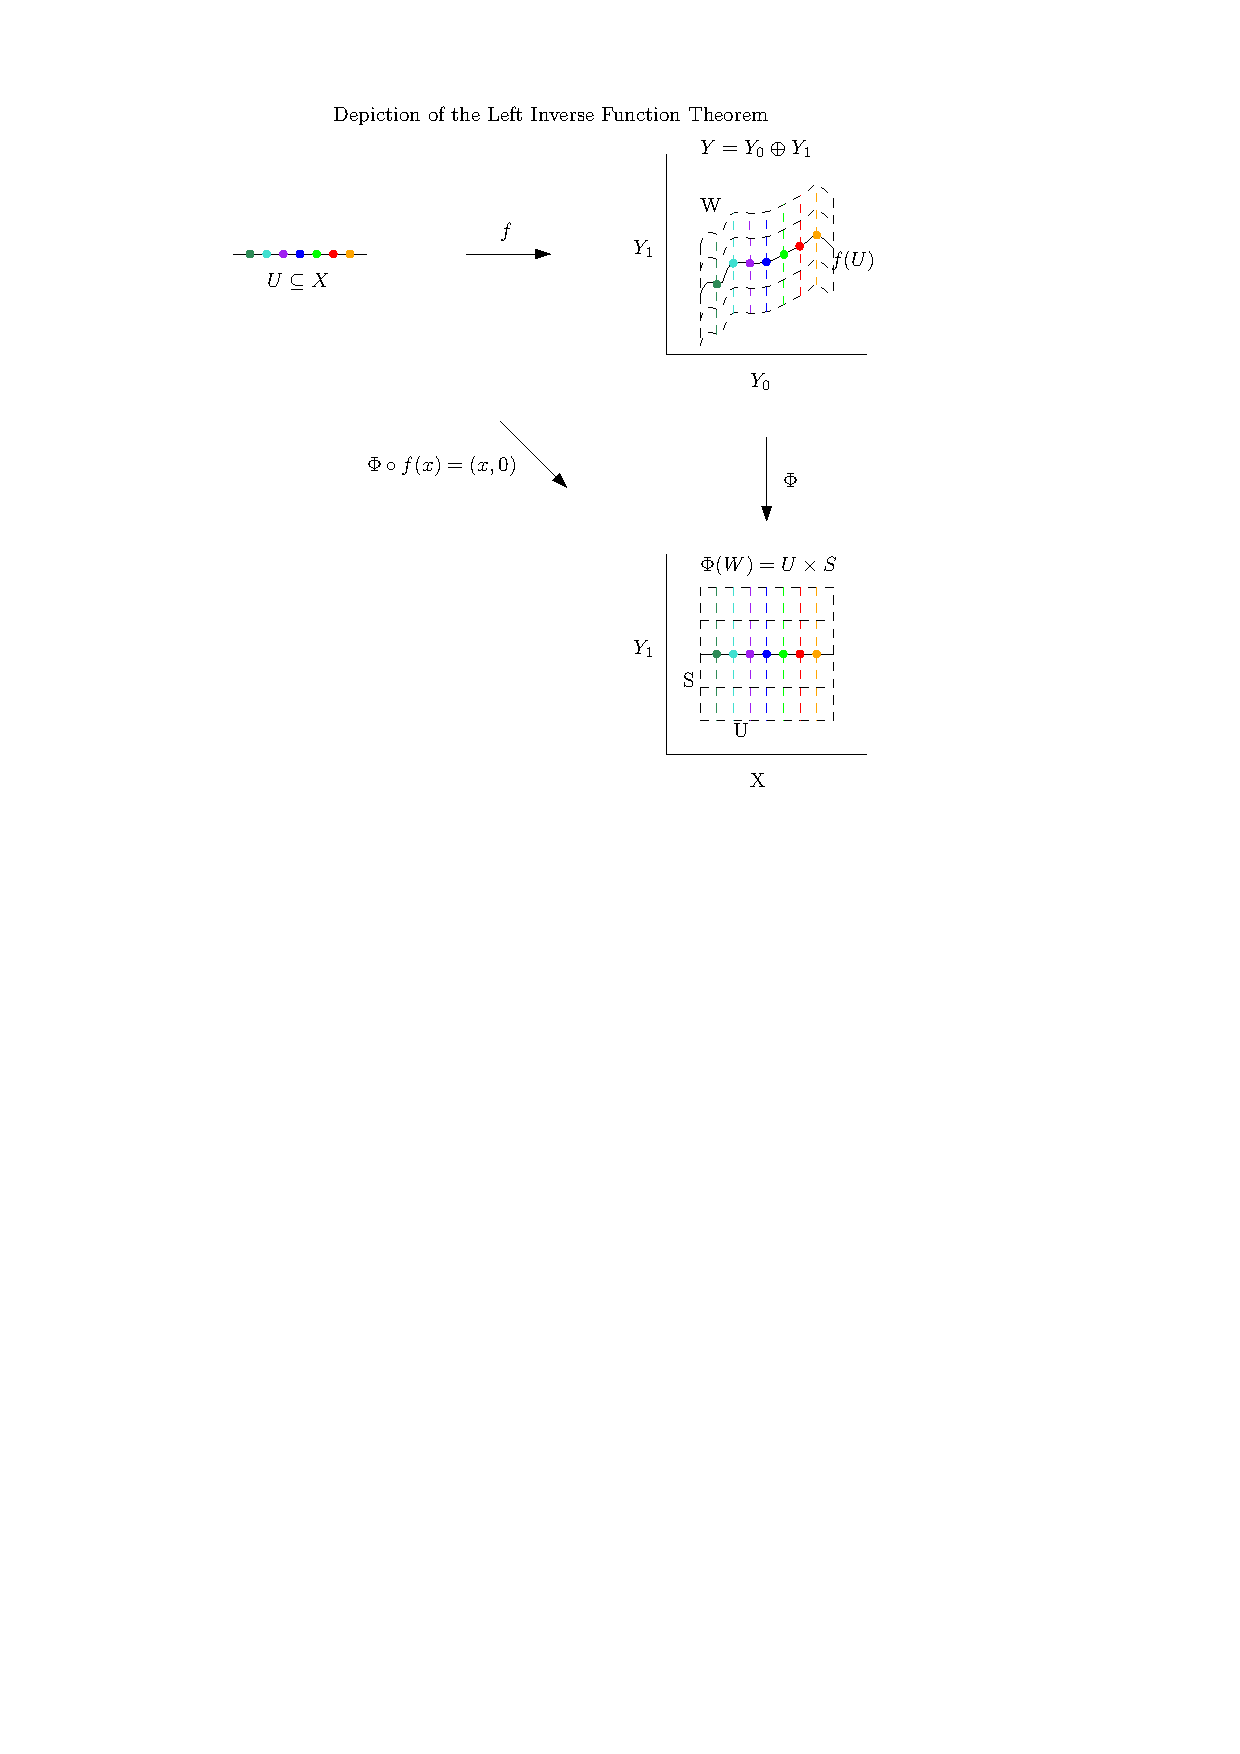
\includegraphics[width=0.55\linewidth]{fig/left_inverse.pdf}
\end{figure}

\begin{proof}
\TODO
\end{proof}

\begin{thm}[flattening map]
Let $X$ and $Y$ be Banach spaces, and suppose that
$Y_0, Y_1 \subset Y$ are nontrivial clsoed subspaces
such that $Y = Y_0 \oplus Y_1$. Suppose further that
$X$ and $Y_0$ are isomophic. Let $M \subset Y$ and
$y_0 \in M$, and let $1 \leq k \leq \infty$. Then the
following are equivalent:
\begin{enumerate}
\item There exist open sets $V \subset X$ and $U \subset Y$
with $y_0 \in U$ and $f \in C^k(U ; Y)$ such that $f :
V \to f(V) = U \cap M$ is a homeomorphism and at $x_0
= f^{-1}(y_0) \in V$ we have that $Df(x_0)$ is injective
with $\ran Df(x_0) = Y_0$.

\item There exists an open set $W \subset Y$ with $y_0 \in W$
and $F \in C^k(W ; X \times Y_1)$ such that $F$ is a
$C^k$ diffeomorphism from $W$ to $F(W)$, $DF(y_0)(Y_0)
= X_0 \times \{0\}$, and
\[
F(W \cap M) = F(W) \cap [X \times \{0\}].
\]

\item There exists an open set $W \subset Y$ with $y_0 \in W$
and $\Phi \in C^k(W ; Y)$ such that $\Phi$ is a $C^k$
diffeomorphism from $W$ to $\Phi(W)$, $D \Phi(y_0) (Y_0)
= Y_0$, and
\[
\Phi(W \cap M) = \Phi(W) \cap Y_0.
\]
\end{enumerate}

Moreover, if either the second or the third items hold, then
the set $V$ from the first item can be chosen such that
$Df(x)$ is injective with $\ran Df(x)$ closed and
complemented in $Y$ for each $x \in V$.
\end{thm}

\begin{proof}
\TODO
\end{proof}

\begin{thm}[right inverse function theorem]
Let $X$ and $Y$ be Banach spaces. Suppose that $\emptyset
\neq U \subset X$ is open and $f \in C^k (U ; Y)$ for
some $1 \leq k \leq \infty$. Let $x_0 \in U$,
$y_0 = f(x_0) \in Y$, and suppose that $\{0\} \neq
\ker Df(x_0) \subset X$. Then the following
are equivalent:

\begin{enumerate}
\item The map $Df(x_0) \in \L(X; Y)$ is surjective with
$\ker Df(x_0)$ complemented in $X$. That is, $Df(x_0)
\in \L_R(X; Y)$.

\item There exist nontrivial closed subspace $X_0, X_1
\subset X$ with $X = X_0 \oplus X_1$ and $P \in \L(X)$
the projection onto $X_0$ and open sets $x_0 \in \tilde{U}
\subset U$, $y_0 \in W \subset Y$, and $Px_0 \in V \subset X_0$
such that the map $G : \tilde{U} \to Y \times X_0$
given by $G(x) = (f(x), Px)$ is a $C^k$ diffeomorphism
onto $W \times V \subset Y \times X_0$. Moreover, for $x
\in \tilde{U}$, we have that $DG(x) (X_1) = Y \times \{0\}$,
and the restriction $DG(x) \vert_{X_1} : X_1 \to Y \times
\{0\}$ is an isomorphism.

\item There exist nontrivial closed subspace $X_0, X_1 \subset
X$ with $X = X_0 \oplus X_1$ and $P \in \L(X)$ the projection
onto $X_0$, open sets $x_0 \in \tilde{U} \subset U$,
$y_0 \in W \subset Y$, and $P x_0 \in V \subset X_0$, and
a map $F \in C^k (W \times V ; X)$ such that $F$ is a
$C^k$ diffeomorphism from $W \times V$ to $F(W \times V)
= \tilde{U}$, $F(y_0, Px_0) = x_0$, and
\[
f(F(y, v)) = y
\]
for all $(y, v) \in W \times V$. Moreover, for all
$(w, v) \in W \times V$ we have that $DF(w, v) (Y \times
\{0\}) = X_1$ and the restriction $DF(w, v) \vert_{Y \times
\{0\}} : Y \times \{0\} \to X_1$ is an isomorphism.

\item There exists an open set $y_0 \in W \subset Y$ and
a map $g \in C^k(W; X)$ such that $g(y_0) = x_0$, $g(W)
\subset U$, and $f(g(y)) = y$ for all $y \in W$.

\item There exists an open set $x_0 \in \tilde{U} \subset U$
such that $Df(x) \in \L(X; Y)$ is surjective with
$\ker Df(x)$ complemented in $X$ for each $x \in \tilde{U}$.
\end{enumerate}
Moreover, in any and hence every case, the $X_i$ spaces
from the second and third items can be taken with $X_0
= \ker Df(x_0)$, and the maps $g, F, G$ can be aken to be
related via $F^{-1} = G$ and $g(y) = F(y, P x_0)$.
\end{thm}

\begin{figure}[!ht]
  \centering
  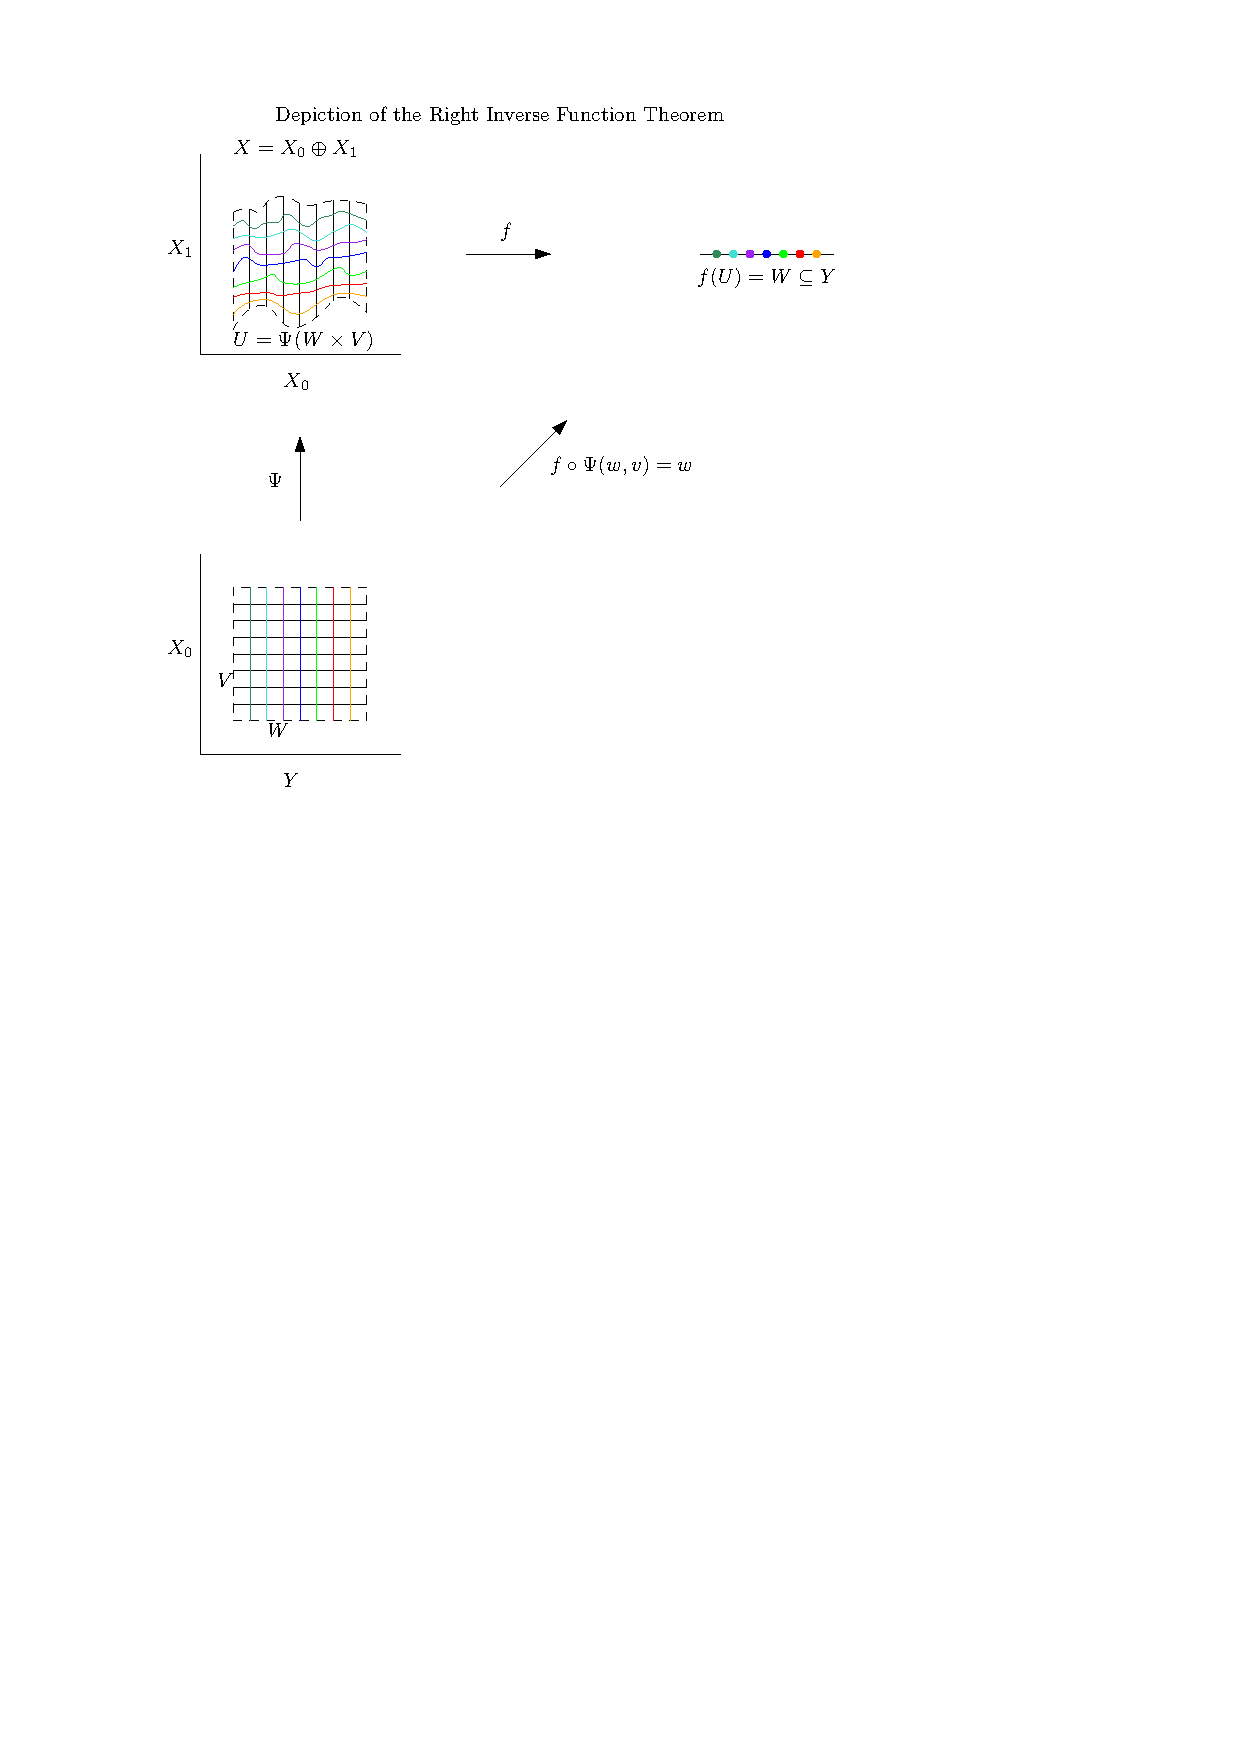
\includegraphics[width=0.55\linewidth]{fig/right_inverse.pdf}
\end{figure}

\begin{proof}
\TODO
\end{proof}

\begin{thm}[Constant rank theorem]
Let $X$ and $Y$ be nontrivial Banach spaces, and suppose 
that $X_0,X_1 \subset X$ and $Y_0,Y_1 \subset Y$ are 
nontrivial closed subspaces such that $X = X_0 \oplus 
X_1$ and $Y = Y_0 \oplus Y_1$.  Write $P_{X_i}$ and 
$P_{Y_i}$ for the projectors onto $X_i$ and $Y_i$, 
respectively, for $i=0,1$.  Let $U \subset X$ be 
open and $x_0 \in U$.  Suppose that $f \in C^k(U;Y)$ 
for $1 \le k\le \infty$ is such that $\ker Df(x_0) = 
X_0$ and $\ran Df(x_0) = Y_0$, and write $y_0 = f(x_0)$.  
Further suppose that $f$ satisfies the ``constant rank 
condition'':
\begin{equation*}
Df(x) (X_1) = \ran Df(x) \text{ for all }x \in U. 
\end{equation*}
Then there exist open sets $x_0 \in \tilde{U} \subset U$ 
and $y_0 \in S \subset Y$ such that $f(\tilde{U}) 
\subset S$ and the following hold.
\begin{enumerate} 
\item There exist open sets $P_{Y_0} y_0 \in W \subset 
Y_0$ and $P_{X_0} x_0 \in V \subset X_0$ and a $C^k$ 
diffeomorphism $\Psi: W \times V \to \tilde{U}$ with 
$\Psi(P_{Y_0} y_0, P_{X_0} x_0) = x_0$.

\item There exists a $C^k$ diffeomorphism $\Phi : S \to 
\Phi(S) \subset Y_0 \times Y_1$ with  
and $\Phi(y_0) = (P_{Y_0} y_0, 0)$.

\item We have that 
\begin{equation*}
\Phi \circ f \circ \Psi(w,v) = (w,0) \text{ for all } 
(w, v) \in W \times V.
\end{equation*}
\end{enumerate}
\end{thm}

Prove the constant rank theorem by arguing as follows.

NOTE: the final forms of the objects you're after won't 
appear clearly until step 4. For instance, don't assume 
that the $W$ from step 1 is the $W$ you're after; you 
may need to shrink it.



\begin{enumerate}
\item Set $w_0 = P_{Y_0} y_0 \in Y_0$ and $v_0 = P_{X_0} 
x_0 \in X_0$, and define the maps $f_i = P_{Y_i} \circ f$ 
for $i=0,1$.  Prove that there exist open sets $x_0 \in 
\tilde{U} \subset U$, $w_0  \in W \subset Y_0$, and 
$v_0 \in V \subset X_0$ with $V$ connected, and a $C^k$ 
diffeomorphism $\Psi : W \times V \to \Psi(W\times V) = 
\tilde{U}$ such that $\Psi(w_0, v_0) = x_0$, 
\begin{equation*} 
f_0(\Psi(w,v)) = w \text{ for all }(w,v) \in W \times V,   
\end{equation*}
and 
\begin{equation*} 
D\Psi(w,v) \vert_{Y_0 \times \{0\}} \to X_1 \text{ is an 
isomorphism for all } (w,v) \in W \times V.
\end{equation*}

\item Define $F : W \times V \to Y$ via $F = f \circ \Psi$. 
Prove the following for all $(w,v) \in W \times V$.
\begin{enumerate}
\item $F(w,v) = w + \eta(w,v)$ for some $\eta \in C^k
(W \times V ; Y_1)$.
\item $\ran Df(\Psi(w,v)) = \ran DF(w,v) = DF(w,v)(Y_0 
\times \{0\})$.
\item The map  $T \in \L(Y ; Y_0 \times \{0\})$ defined 
by $Th = (P_{Y_0} h, 0)$ is a left-inverse of the restriction 
$DF(w,v) \vert_{Y_0 \times \{0\}}$.
\item $DF(w,v) \vert_{Y_0 \times \{0\}}$ is injective 
with closed and complemented range given by
\[
\ran DF(w,v) = \ran Df(\Psi(w,v)).
\]
\end{enumerate}

\item Prove that  $DF(w,v) \circ T = I \text{ on } 
DF(w,v)(Y_0 \times \{0\}) = \ran DF(w,v) \subset Y$  
for $(w,v) \in W \times V$.  Use this to deduce that 
$D_2 \eta(w,v) =0$ and hence that $D_2 F(w,v) =0$ for 
$(w,v) \in W \times V$.  In turn, deduce that 
\begin{equation*}
F(w,v) = F(w,v_0) \text{ for all }(w,v) \in W \times V.
\end{equation*}

\item Define $G: W \to Y$ via $G(w) = F(w,v_0)$.  
Apply the left inverse function theorem (HW1 P1) 
to complete the proof.
  
  

\end{enumerate}

\begin{proof}
{
\newcommand{\py}{{P_{Y_0}}}
\newcommand{\pyy}{{P_{Y_1}}}
\newcommand{\px}{{P_{X_0}}}
\newcommand{\pxx}{{P_{X_1}}}
\begin{enumerate}
\item Define a map $g: U \to Y_0 \times X_0$ by 
\[
g(x) = \left( P_{Y_0}(f(x)), P_{X_0}x \right).
\]
Then, the derivative of $g$ at $x \in U$ is 
\[
Dg(x) h = (P_{Y_0} \circ Df(x) (h), P_{X_0} h).
\]
Claim that $Dg(x_0)$ is an isomorphism. For surjectivity, 
consider $(y, x) \in Y_0 \times X_0$. Since $\ran Df(x_0) = Y_0$,
there is $v \in X$ such that $Df(x_0) (v) = y$. 
Since $\ker Df(x_0) = X_0$ and $X_0 \oplus X_1 = X$, 
we can assume WLOG 
that $v \in X_1$. Now, let $h = v + x$. Then,
\[
\begin{aligned}
Dg(x_0) h 
= (\py \circ Df(x_0) (v) , \px x) 
= (y, x).
\end{aligned}
\]
Therefore, $Dg(x_0)$ is surjective. For injective, consider 
$Dg(x_0) h = (0, 0)$ for some $h \in X$. It follows that 
$\px h = 0$ and $Df(x_0) h = Df(x_0) (\pxx h) = 0$. 
This implies $\pxx h \in X_1 \cap \ker Df(x_0) = X_1 \cap X_0$.
Therefore, $h = 0$ and $Dg(x_0)$ is indeed an isomorphism.

Now, the inverse function theorem gives bounded and open sets 
$x_0 \in U' \subset U$ such that $g: U' \to 
g(U')$ is a bi-Lipschitz homeomorphism, $Dg(x)$ an 
isomorphism for all $x \in U'$, and $g^{-1}$ differentiable 
on $g(U')$ with 
\[
Dg^{-1}(w, v) = [Dg(g^{-1}(w, v))]^{-1}.
\]
Further let $w_0 \in W \subset Y_0$ and 
$v_0 \in V \subset X_0$ be small open balls such
that $W \times V \subset g(U')$, 
$\Psi: W \times V \to X$ be the inverse of $g$, and 
$\tilde{U} = g(W \times V)$. 
Now $x_0 \in \tilde{U}$ since $g(x_0) = (w_0, v_0)$,
$v_0 \in V \subset X_0$ connected, and
$\Psi : W \times V \to \tilde{U}$
is a $C^k$ diffeomorphism.
Additionally, for all $(w, v) \in W \times V \subset Y_0 \times X_0$,
we have let $\Psi(w, v) = x$ for some $x \in \tilde{U}$. Then, we 
know $\py \circ f(x) = w$. Therefore, 
\[
f_0(\Psi(w, v)) = w 
\]
for all $(w, v) \in W \times V$.

To show $D \Psi(w, v) \vert_{Y_0 \times \left\{ 0 \right\}} \to X_1$
is an isomorphism for all $(w,v) \in W \times V$, 
note that $D\Psi(w,v)$ is already an 
isomorphism and thus injective. Now for any $u \in X_1$, 
we have 
\[
Dg(\Psi(w, v))u = (\py \circ Df(\Psi(w, v))(u), \px u).
\]
Note that $\px u = 0$ since $u \in X_1$ and 
$\py \circ Df(\Psi(w, v))(u) \in Y_0$. 
Also, $Dg(\Psi(w, v))$
is an isomorphism, so 
\[
D\Psi(w, v) (\py \circ Df(\Psi(w, v))(u), 0) = u.
\]
This implies  
that $D\Psi(w, v) (Y_0 \times \left\{ 0 \right\}) = X_1$.
Therefore, $D \Psi(w, v) \vert_{Y_0 \times \left\{ 0 \right\}} \to X_1$
is indeed an isomorphism for all $(w,v) \in W \times V$.

\item \begin{enumerate}
\item Define $\eta: W \times V \to Y_1$ by 
\[
\eta(w, v) = \pyy \circ f(\Psi(w, v)) = f_1 \circ \Psi(w, v).
\]
Then, $\eta \in C^k(W \times V ; Y_1)$ and 
\[
F(w, v) = f (\Psi(w, v)) = f_0 (\Psi (w, v)) 
+ f_1 (\Psi (w, v)) = w + \eta(w, v),
\]
as desired.

\item First of all, it follows from the chain rule that 
for all $(w,v) \in W \times V$,
\[
DF(w, v) = Df(\Psi(w, v)) D\Psi(w, v).
\]
Recall from part 1 that $D\Psi(w, v)$ is isomorphism, 
so $\ran DF(w, v) = \ran Df(\Psi(w, v))$.
Additionally, we have $Df(\Psi(w, v))(Y_0 \times \left\{ 0 \right\}) = X_1$
and note that $Df(x)(X_1) = \ran Df(x)$ for all $x \in \tilde{U}$.
Therefore,
\[
Df(\Psi(w, v)) D\Psi(w, v) (Y_0 \times \left\{ 0 \right\})
= Df(\Psi(w, v))(X_1) = \ran Df(\Psi(w, v)).
\]
This implies that 
\[
\ran Df(\Psi(w, v)) = \ran DF(w, v) = DF(w, v) 
(Y_0 \times \left\{ 0 \right\}),
\]
as desired.

\item Let $y \in Y_0$. We want to show that 
$T \circ DF(w, v) (y, 0) = (y, 0)$. Again, 
note that 
\[
DF(w, v) = Df(\Psi(w, v)) D\Psi(w, v).
\]
Suppose $D \Psi(w, v)(y, 0) = h$. 
As shown in part 1, we have 
\[
Dg(x) h = (\py \circ Df(x) (h), \px h).
\]
for all $x \in U$.
It follows that 
$\py \circ Df(\Psi(w, v)) h = y$ and $\px h = 0$. 
Therefore, 
\[
\begin{aligned}
  T \circ DF(w, v) (y, 0) 
  = T \circ Df(\Psi(w, v)) h 
  = (\py \circ Df(\Psi(w, v)) h, 0) = (y, 0).
\end{aligned}
\]
This implies that $T \in \L(Y; Y_0 \times \left\{ 0 \right\})$
defined by $Th = (\py h, 0)$ is a left inverse of $DF(w, v)$
restricted on $Y_0 \times \left\{ 0 \right\}$.

\item Since $DF(w, v) \vert_{Y_0 \times \left\{ 0 \right\}}$ 
has a left inverse, $DF(w, v) \vert_{Y_0 \times \left\{ 0 \right\}}$
is injective with its range closed and complemented. In addition,
from part (b), we know that $\ran DF(w, v) = \ran Df(\Psi(w, v))$,
as desired.

\end{enumerate}

\item Since $DF(w, v) \vert_{Y_0 \times \left\{ 0 \right\}}$
is injective with closed and complemented range given by 
\[
\ran DF(w, v) = \ran Df(\Psi(w, v)),
\]
$DF(w,v) : 
Y_0 \times \left\{ 0 \right\} \to \ran DF(w, v)$ 
is an isomorphism.
In particular, it is invertible. Since $T$ is the a left-inverse,
$T$ must also be the right inverse. Therefore, 
$DF(w, v) \circ T = I$ on $DF(w, v)(Y_0 \times \left\{ 0 \right\})
= \ran DF(w, v) \subset Y$ for all $(w, v) \in W \times V$.

Next we show $D_2 \eta (w, v) = 0$. Let $h \in X_0$ be 
arbitrary. By the definition of $\eta$, we have 
\[
\begin{aligned}
D_2 \eta (h) 
&= \pyy \circ Df(\Psi(w, v)) D_2 \Psi(w, v) h \\
&= \pyy \circ Df(\Psi(w, v)) D\Psi(0, h) \\
&= \pyy \circ DF(w, v) (0, h).
\end{aligned}
\]
Now, using the fact that $DF(w, v) \circ T = I$, we have 
\[
\begin{aligned}
DF(w, v) (0, h) 
&= DF(w, v) \circ T \circ DF(w, v) (0, h) \\ 
&= DF(w, v) (\py \circ DF(w, v)(0, h), 0).
\end{aligned}
\]
Claim that $\py \circ DF(w, v) (0, h) = 0$. Indeed, 
let $D\Psi(w, v) (0, h)  = u$. Note that $D\Psi(w, v) 
= [Dg(\Psi(w, v))]^{-1}$ and $Dg(x) k = (\py \circ Df(x) k, 
\px k)$ for all $x \in U$ and $k \in X$. 
It follows that $\py \circ Df(\Psi(w, v)) u = 0$.
Therefore, 
\[
\py \circ DF(w, v) (0, h) = \py \circ Df(\Psi(w, v)) 
D\Psi(w, v) (0, h) = \py \circ Df(\Psi(w, v)) u = 0.
\]
Hence, 
\[
D_2 \eta (h) = \pyy \circ DF(w, v) (0, h) 
= \pyy \circ DF(w, v)(0, 0) 
= 0.
\]
This implies that $D_2 \eta(w, v) = 0$, as desired.

Now, by the equality in part 2(a), we have 
\[
D_2 F(w, v) = D_2 \eta(w, v) = 0.
\]
for all $(w, v) \in W \times V$.
Now by the mean value theorem,
\[
\begin{aligned}
\norm{F(w, v) - F(w, v_0)} 
\leq \norm{v - v_0} \sup_{h \in V} \norm{D_2 F(w, h)} 
= 0.
\end{aligned}
\]
Therefore, $F(w, v) = F(w, v_0)$ for all $(w, v) 
\in W \times V$.

\item Define $G : W \to Y$ by $G(w) = F(w, v_0)$. Claim 
that $DG(w_0) \in \L(Y_0; Y)$ is injective with 
$\ran DG(w_0)$ closed and complemented. Indeed, 
for any $Y_0 \in X$, we have 
\[
\begin{aligned}
DG(w)h = D_1 F(w, v_0)h = DF(w, v_0)(h, 0).
\end{aligned}
\]
Note that in part 2(d), we have shown that 
$DF(w, v) \vert_{Y_0 \times \left\{ 0 \right\}}$
is injective with closed and complemented range. 
Therefore, $DG(w_0)$ is also injective with 
closed and complemented range. In fact,
\[
\ran DG(w_0) = DF(w_0, v_0) (Y_0 \times \left\{ 0 \right\})
= \ran Df(\Psi(w_0, v_0)) = \ran Df(x_0) = Y_0.
\]
Note that $Y_0 \oplus Y_1 = Y$.
Now, by the left inverse function theorem, thre exists 
open sets $w_0 \in \tilde{W} \subset W$, 
$0 \in R \subset Y_1$, and 
$S \subset Y$ and a map $\Phi \in C^k(S \to Y_0 \times Y_1)$
such that $\Phi$ is a $C^k$ diffeomorphism from $S$
to $\Phi(S) = \tilde{W} \times R \subset Y_0 \times Y_1$,
$G(\tilde{W}) \subset S$, and 
\[
\Phi(G(w)) = (w, 0) 
\]
for all $w \in \tilde{W}$. In particular,
\[
\Phi(y_0) = \Phi(F(w_0, v_0)) = \Phi(G(w_0)) = (w_0, 0),
\]
and 
\[
\Phi \circ f \circ \Psi(w, v) = \Psi(F(w, v_0)) = 
\Psi(G(w)) = (w, 0)
\]
for all $w \in \tilde{W}$. This completes the proof with 
$\tilde{W}$ being the desired $W$ in the problem statement.
\end{enumerate}  

}
\end{proof}

Below is a naming sanity check for the constant rank theorem.

\begin{thm}
Let $X = \F^{n+r}$ and $Y = \F^{m+r}$ for $1\le m,n,r$.  
Suppose that $U \subset X$ is open with $x_0 \in U$, 
and $f \in C^k(U;Y)$ for $1 \le k \le \infty$.   
Write  $\ker Df(x_0) = X_0$ and $\ran Df(x_0) = Y_0$.  
In finite dimensions all subspaces are closed and 
complemented, so we write $X = X_0 \oplus X_1$ and 
$Y = Y_0 \oplus Y_1$.  Prove that the following are 
equivalent.
\begin{enumerate}
 \item There exists an open set $x_0 \in \tilde{U} 
 \subset U$ such that $\operatorname{rank} Df(x) = r$ 
 for all $x \in \tilde{U}$.
 \item We have that $\dim X_1 = \dim Y_0 = r$, 
 and there exists an open set $x_0 \in \tilde{U} 
 \subset U$ such that 
\begin{equation*}
 Df(x)(X_1) = \ran Df(x) \text{ for all }x \in \tilde{U}.
\end{equation*}
\end{enumerate}
NOTE: this equivalence is where the constant rank 
theorem gets its name.
\end{thm}

\begin{proof}
{
\newcommand{\py}{{P_{Y_0}}}
\newcommand{\pyy}{{P_{Y_1}}}
\newcommand{\px}{{P_{X_0}}}
\newcommand{\pxx}{{P_{X_1}}}
(1) $\implies$ (2). Suppose there exists an open set 
$x_0 \in U' \subset U$ such that $\rank Df(x) = r$
for all $x \in U'$. Note that $\ker Df(x_0) = X_0$, 
$\ran Df(x_0) = Y_0$. 
This implies that $\dim X_1 = \dim Y_0 = \rank Df(x_0) = r$.
Additionally, 
this implies that $Df(x_0)$ is injective with closed 
range when restricted to $X_1$. Since the set of 
injective maps with closed range is open and 
$x_0 \in U'$ is open, we can find open set 
$x_0 \in \tilde{U} \subset U'$
so small that $Df(x)$ is injective with closed range 
when restricted to $X_1$ for all $x \in \tilde{U}$. 
It follows that for all $x \in \tilde{U}$, we have 
\[
\dim Df(x) (X_1) \geq \dim X_1 = r.
\]
However, note that 
$\rank Df(x) = \dim \ran Df(x) = r$ 
and $Df(x) (X_1) \subset \ran Df(x)$ for all $x \in \tilde{U}$.
Therefore,
\[
Df(x) (X_1) = \ran Df(x)
\] 
for all $x \in \tilde{U}$.

(2) $\implies$ (1).
Suppose $\dim X_1 = \dim Y_0 = r$ and there exists an open 
set $x_0 \in U' \subset U$ such that 
\[
Df(x)(X_1) = \ran Df(x)
\]
for all $x \in U'$.
Let $y_0 = f(x_0)$.
Then, by constant rank theorem in problem 4, 
there exists open sets 
$x_0 \in \tilde{U} \subset U'$, $\py y_0 \in W \subset Y_0$,
and $\px x_0 \in V \subset X_0$, and a $C^k$ diffeomorphism 
$\Psi: W \times V \to \tilde{U}$. 
Additionally, let $F : W \times V \to Y$ by 
$F = f \circ \Psi$. Then for all $x \in \tilde{U}$,
we know $x = \Psi(w, v)$ for some $(w,v) \in W \times V$.
Also, $\ran Df(x) = DF(w, v)(Y_0 \times \left\{ 0 \right\})$
with $DF(w, v) \vert_{Y_0 \times \left\{ 0 \right\}}$ an 
isomorphism from $Y_0 \times \left\{ 0 \right\}$ to 
$DF(w, v) (Y_0 \times \left\{ 0 \right\})$. 
It follows that 
\[
\rank Df(x) = \dim \ran Df(x) 
= \dim DF(w, v) \vert_{Y \times \left\{ 0 \right\}}
= \dim Y_0 = r.
\]
for all $x \in \tilde{U}$. This completes the proof.
}

\end{proof}

We define now a nonlinear version of linear dependence.
\begin{defi}
Assume that $m,n \in \N \setminus \{0\}$.  Let 
$\emptyset \neq U \subset \R^n$, and suppose that 
$f_i: U \to \R$ for $i=1,\dotsc,m$.  Write 
$f: U \to \R^m$ via $f = (f_1,\dotsc,f_m)$.  
We say that $\{f_1,\dotsc,f_m\}$ are functionally 
dependent in $U$ if there exists an open set 
$V \subset \R^m$ with $f(U) \subset V$ and 
a function $g \in C^1(V;\R)$ such that 
\begin{equation*}
 g(f_1(x),\dotsc,f_m(x)) =0 \text{ for all } x\in U
\end{equation*}
and $\nabla g(y) \neq 0$ for all $y \in V$.
\end{defi}

\begin{thm}
Let $\emptyset \neq U \subset \R^n$ and $f \in 
C^1(U;\R^m)$.

\begin{enumerate}

\item Prove that if $\{f_1,\dotsc,f_m\}$ are functionally 
dependent on $U$, then for each $x_0 \in U$ there exists 
an open set $V \subset U$ with $x_0 \in V$,  a function  
$h \in C^1(W;\R)$, where $W\subset \R^{m-1}$ is an open 
set, and an index $i \in\{1,\dotsc,m\}$ such that
\begin{equation*}
f_i(x) = h(f_1(x),\dotsc,f_{i-1}(x),f_{i+1}(x),
\dotsc,f_m(x)) \text{ for all }x \in V.
\end{equation*}
In other words, at least one of the functions can be 
written in terms of the other functions.



\item Prove that if  $m \le n$ and $\{f_1,\dotsc,f_m\}$ 
are functionally dependent on $U$, then 
\begin{equation*}
\text{rank}(Df(x)) \le m-1 \text{ for all }x \in U.
\end{equation*}



\item Suppose that $1 \le k < \min\{m,n\}$ and that $Df$ 
is of constant rank $k$ on $U$.  Prove that for each 
$x_0\in U$ there exists an open set $Z \subset U$ 
such that $x_0 \in Z$ and  $\{f_1,\dotsc,f_m\}$ are 
functionally dependent in $Z$.   
\end{enumerate}
  
\end{thm}

\begin{proof}
{
\newcommand{\py}{{P_{Y_0}}}
\newcommand{\pyy}{{P_{Y_1}}}
\newcommand{\px}{{P_{X_0}}}
\newcommand{\pxx}{{P_{X_1}}} 
\begin{enumerate}
\item Let $x_0 \in U$ and $y_0 = f(x_0)$. Then, we have 
\[
\nabla g(y_0) = (D_1 g (y_0), \dots, D_m g(y_0)) \neq 0.
\]
It follows that there exists an index $i \in 
\left\{ 1, \dots, m \right\}$ such that $D_i g(y_0) \neq 0$.
WLOG assume $i = 1$.
Now, by the implicit function theorem, there exists open 
sets $(f_2(x_0), \dots, f_m(x_0)) \in W \subset \R^{m-1}$, 
$f_1(x_0) \in \tilde{V} \subset \R$, and $0 \in S \subset \R$
and $h \in C^1(W ; \R)$ such that 
\[
h(f_2(x_0), \dots, f_m(x_0)) = f_1(x_0)
\]
and 
$(y_2, \dots, y_m, h(y_2, \dots, y_m, z)) \in W 
\times \tilde{V}$ for all $(y_2, \dots, y_m, z) \in W \times S$.
Additionally,
\[
g(y_2, \dots, y_m, h(y_2, \dots, y_m, z)) = z 
\]
for all $(y_2, \dots, y_m, z) \in W \times S$.
Also, if $(y_1, y_2, \dots, y_m) \in \tilde{V} \times W$
such that 
\[
g(y_1, y_2, \dots, y_m) = z
\]
for some $z \in S$,
then $y_1 = h(y_2, \dots, y_m)$. 

Since $f_i \in C^1(U; \R)$ for all $i = 1, \dots, m$, 
we can select open set $x_0 \in V \subset U$ so small that 
$f_1(x) \in \tilde{V}$ and $(f_2(x), \dots, f_m(x)) \in W$
for all $x \in V$. It follows that 
\[
g(f_1(x), \dots, f_m(x)) = 0
\]
for all $x \in V$. This implies that $f_1(x) = h(f_2(x), 
\dots, f_m(x))$ as argued above. 

\item Since $g(f_1(x), \dots, f_m(x)) = g(f(x)) = 0$
for all $x \in U$, we have 
\[
\nabla g(f(x)) \circ Df(x) = 0.
\]
Notice that $f(U) \subset V$ and $\nabla g(y) \neq 0$ 
for all $y \in V$. It then follows that 
$\nabla g(f(x)) (\R^m) \neq 0$
for all $x \in U$.
Suppose for contradiction that $\rank Df(x) = m$ for 
some $x_0 \in U$. Then, $Df(x_0) (\R^n) = \R^m$.
However, this will imply that $\nabla g(f(x_0)) \circ Df(x_0)
\neq 0$, a contradiction. Therefore, 
\[
\rank Df(x) \leq m - 1
\]
for all $x \in \tilde{U}$. 

\item Suppose that $1 \leq k < \min \left\{ m, n \right\}$
and that $\rank Df(x) = k$ for all $x \in U$. 
Fix $x_0 \in U$ and write $\ker Df(x_0) = X_0$ and 
$\ran Df(x_0) = Y_0$, where $X_0$ and $Y_0$ are complemented 
with $X_0 \oplus X_1 = \R^n$ and 
$Y_0 \oplus Y_1 = \R^m$. 
By problem 5, we know that 
$\dim X_1 = \dim Y_0 = k$ and 
there exists and open set $x_0 \in \tilde{U} \subset U$ 
such that 
\[
Df(x)(X_1) = \ran Df(x) 
\]
for all $x \in \tilde{U}$. 

Note that $k < \min \left\{ m, n \right\}$, so $X_i$ and 
$Y_i$ are nontrivial for $i = 0, 1$.
Set $y_0 = f(x_0)$. By constant rank theorem in problem 4, 
there exists open sets $x_0 \in Z \subset U$ and 
$y_0 \in S \subset Y$, $\py y_0 \in W \subset Y_0$, 
and $\px x_0 \in V \subset X_0$, and $C^k$ diffeomorphisms 
$\Psi: W \times V \to Z$ with $\Psi(\py y_0, \px x_0) = x_0$,
$\Phi: S \to Y_0 \times Y_1$ with $\Phi(y_0) = (\py y_0, 0)$,
and 
\[
\Phi \circ f \circ \Psi(w, v) = (w, 0)
\]
for all $w \in W$. Now define $g: S \to \R$ 
by 
\[
g(y) = \pi_{k+1} \circ \Phi(y),
\]
where $\pi_{k+1}$ is projection onto the $(k+1)$-th index. 
Notice first for all $y \in S$, we have 
\[
\nabla g(y) = \pi_{k+1} \circ D\Phi(y).
\]
Since $D\Phi(y)$ is an isomorphism and $\pi_{k+1}$ has 
nonzero range, $\nabla g(y) \neq 0$ for all $y \in S$. 
Additionally, for each $x \in Z$, there exists $(w, v)
= \Psi^{-1}(x) \in W \times V$
Therefore, for all $x \in Z$, 
\[
\begin{aligned}
g(f(x)) = \pi_{k+1} \circ \Phi \circ f \circ \Psi(\Psi^{-1}(x)) 
= \pi_{k+1} (w, 0) = 0.
\end{aligned}
\]
This shows that $\left\{ f_1, \dots, f_m \right\}$
are functionally dependent in $Z$.
\end{enumerate}

}
\end{proof}

\section{Measure and integration}

\subsection{Introduction to abstrct measure theory}

\subsubsection{Basic definitions}

\begin{defi}
  Let $X$ be a set.
  \begin{enumerate}
    \item An \textbf{algebra} on $X$ is $\afk \subset
    \P(X)$ such that
    \begin{enumerate}
      \item $\emptyset \in \afk$.
      \item $E \in \afk$ implies $E^c \in \afk$.
      \item $E, F \in \afk$ implies $E \cup F \in \afk$.
    \end{enumerate}

    \item A \textbf{$\sigma$-algebra} is an algebra
    $\mf \subset \P(X)$ such that if
    $E_k \in \mf$ for all $k \in \N$, then
    $\cupinfk E_k \in \mf$.

    \item A pair $(X, \mf)$ with $\mf$ a $\sigma$-algebra
    on $X$ is called a \textbf{measurable space}.
  \end{enumerate}
\end{defi}

\begin{thm}
  Let $X$ be a set.
  \begin{enumerate}
    \item Suppose $A \neq \emptyset$ is a set and
    $\mf_\alpha$ is $\sigma$-algebra for each $
    \alpha \in A$, then $\mf = \bigcap_{\alpha \in A}
    \mf_\alpha$ is a $\sigma$-algbera on $X$.

    \item Suppose $F \subset \P(X)$, there is unique
    smallest $\sigma$-algebra $\mf$ on $X$ such that
    $F \subset \mf$. Write $\mf = \sigma(F)$ and call
    this the $\sigma$-algebra generated by $F$.
  \end{enumerate}
\end{thm}

\begin{thm}
  Let $X$ and $Y$ be sets and $f: X \to Y$.
  \begin{enumerate}
    \item Suppose $\mf$ is a $\sigma$-algebra on $X$
    and set
    \[
    \nf = \left\{ E \subset Y:
    f^{-1}(E) \in \mf \right\}.
    \]
    Then, $\nf$ is a $\sigma$-algebra on $Y$.
    Call this the \textbf{push-forward} of $\mf$
    by $f$.

    \item Suppose $\nf$ is a $\sigma$-algebra
    on $Y$ and set
    \[
    \mf = \left\{ f^{-1}(E) : E \in \nf \right\}.
    \]
    Then, $\mf$ is a $\sigma$-algebra on $X$. Call
    this the \textbf{pull-back} of $\nf$ by $f$.
  \end{enumerate}
\end{thm}

\begin{defi}
  Let $A \neq \emptyset$ be a set.
  \begin{enumerate}
    \item Let $Y$ be a set and $X_\alpha$ be sets
    with $\sigma$-algebra $\mf_\alpha$ for all
    $\alpha \in A$. Suppose $g_\alpha : X_\alpha
    \to Y$ for all $\alpha \in A$. Define
    \[
    \sigma \left( \left\{ E \subset Y: g_\alpha^{-1}(E)
    \in \mf_\alpha \text{ for all $\alpha \in A$}
    \right\} \right)
    \]
    to be the \textbf{push-forward} of $\left\{ g_\alpha
    \right\}_{\alpha \in A}$.

    \item Let $X$ be a set and $Y_\alpha$ be sets with
    $\sigma$-algebra $\nf_\alpha$ for all $\alpha \in A$.
    Suppose $f_\alpha : X \to Y_\alpha$ for all $\alpha \in
    A$. Define
    \[
    \sigma \left( \left\{ f_\alpha^{-1}(E) :
    E \in \nf_\alpha \text{ for some $\alpha \in A$}
    \right\} \right)
    \]
    to be the \textbf{pull-back} of $\left\{ f_\alpha
     \right\}_{\alpha \in A}$.
  \end{enumerate}
\end{defi}

\begin{defi}
  Let $A \neq \emptyset$ be a set and $X_\alpha$ be sets
  with $\sigma$-algebra $\mf_\alpha$ for all
    $\alpha \in A$. Then on the set $X = \prod_\alpha X_\alpha$
    we define the \textbf{product $\sigma$-algbera}
    $\bigotimes_\alpha \mf_\alpha$ to be the
    pull-back of projection maps
    $\pi_\alpha : X \to X_\alpha$.
\end{defi}
{
\begin{thm}
  Let $A \neq \emptyset$ be a set and $X_\alpha$
  with $\sigma$-algebra $\mf_\alpha$ for all $\alpha
  \in A$. Let $X = \prod_\alpha X_\alpha$ and
  define
  \[
  \mathcal{R} = \left\{ \prod_\alpha M_\alpha:
  M_\alpha \in \mf_\alpha \right\}.
  \]
  Then,
  \begin{enumerate}
    \item $\bigotimes_\alpha \mf_\alpha \subset \sigma
    (\rcal)$. If $A$ countable then $\sigma(\rcal)
    = \bigotimes_\alpha \mf_\alpha$.

    \item Suppose $\mf_\alpha = \sigma(\ecal_\alpha)$
    for all $\alpha \in A$ and let
    \[
    \ecal = \left\{ \pi_\alpha^{-1}(E) :
    E \in \ecal_\alpha \text{ for some $\ecal_\alpha$} \right\}.
    \]
    Then $\bigotimes_\alpha \mf_\alpha = \sigma(\ecal)$.
    Moreover, if $A$ is countable and $X_\alpha \in \ecal_\alpha$
    for all $\alpha \in A$, then $\bigotimes_\alpha \mf_\alpha$
    is generated by $\fcal = \left\{ \prod_\alpha E_\alpha :
    E_\alpha \in \ecal_\alpha \right\}$
  \end{enumerate}
\end{thm}

\begin{proof}
\begin{enumerate}
\item For $E \in \mf_\alpha$, we have
$\pi^{-1}_\alpha (E) = \prod_\beta S_\beta$, where
\[
S_\beta = \begin{cases}
  E & (\beta = \alpha), \\
  X_\beta & (\beta \neq \alpha).
\end{cases}
\]
Then,
\[
\left\{ \pi_\alpha^{-1}(M_\alpha) : M_\alpha
\in \mf_\alpha \right\}
\subset \left\{ \prod_\beta M_\beta: M_\beta \in
\mf_\beta \right\} = \rcal.
\]
This implies that $\bigotimes_\alpha \mf_\alpha \subset
\sigma(\rcal)$.

On the other hand, if $A$ is countable, then
\[
\prod_\alpha M_\alpha =
\bigcap_\alpha \pi_\alpha^{-1} (M_\alpha)
\in \bigotimes_\alpha \mf_\alpha
\]
whenever $M_\alpha \in \mf_\alpha$ for all $\alpha \in A$.
This implies that $\sigma(\rcal) \subset \bigotimes_\alpha
\mf_\alpha$.

\item It is clear that $\sigma(\ecal) \subset \bigotimes_\alpha
\mf_\alpha$. On the other hand, for each $\alpha \in A$, let
\[
  \nf_\alpha = \left\{ E \subset X_\alpha : \pi^{-1}_\alpha
  (E) \in \sigma(\ecal) \right\}
\]
be the push-forward
of $\sigma(\ecal)$ to $X_\alpha$ by $\pi_\alpha$.
It is clear that $\ecal_\alpha \subset \nf_\alpha$.
This implies $\mf_\alpha = \sigma(\ecal) \subset \nf_\alpha$.
In particular, $\pi_\alpha^{-1}(E) \in \sigma(\ecal)$
for all $E \in \mf_\alpha$. This implies that
$\bigotimes_\alpha \mf_\alpha \subset \sigma(\ecal)$.

Now, assume $A$ countable and $X_\alpha \in \ecal_\alpha$
for all $\alpha \in A$. Then let $E \in \mf_\alpha$
for some $\alpha \in A$. We have
$\pi^{-1}_\alpha(E) = \prod_\beta S_\beta$, where
\[
S_\beta = \begin{cases}
  E & (\beta = \alpha), \\
  X_\beta & (\beta \neq \alpha).
\end{cases}
\]
Therefore, $\sigma(\ecal) \subset \sigma(\fcal)$.

On the other hand, since $A$ is countable, we have
\[
\prod_\alpha E_\alpha = \bigcap_\alpha \pi_\alpha^{-1}
(E_\alpha) \in \sigma(\ecal).
\]
This implies that $\sigma(\fcal) \subset \sigma(\ecal)$
and the proof is complete.

\end{enumerate}
\end{proof}
}

\begin{cor}
  If $\mf_i$ is $\sigma$-algebra for $i = 1, 2, 3$, then
  \[
  \mf_1 \otimes (\mf_2 \otimes \mf_3)
  = (\mf_1 \otimes \mf_2) \otimes \mf_3
  = \mf_1 \otimes \mf_2 \otimes \mf_3,
  \]
  since they are all generated by
  \[
  \left\{ M_1 \times (M_2 \times M_3) \right\}
  = \left\{ (M_1 \times M_2) \times M_3 \right\}
  = \left\{ M_1 \times M_2 \times M_3 \right\}.
  \]
\end{cor}

\begin{thm}
  Let $X_1, \dots, X_n$ be metric spaces and
  $X = \prod_{i=1}^n X_i$ be equipped with the ususal
  metric. Then, $\bigotimes_{i=1}^n \bfk_{X_i} \subset
  \bfk_X$. However, if each $X_i$ is separable,
  then $\bfk_X = \bigotimes_{i=1}^n \bfk_{X_i}$.
\end{thm}

\begin{proof}
  We know by the previous theorem that
  $\bigotimes_{i=1}^n \bfk_{X_i}$ is generated
  by $\left\{ \prod_i U_i : U_i \subset X_i \text{ open}
  \right\}$. However, $\prod_i U_i$ is open in $X$.
  Therefore, $\bigotimes_{i=1}^n \bfk_{X_i} \subset \bfk_X$.

  Suppose now each $X_i$ is separable and let $D_i \subset X_i$
  be countable and dense. Consider
  \[
  \ecal_i = \left\{ B(x_i, r): \text{ $X_i \in D_i$,
  $r = \infty$ or $r \in \Q^+$} \right\},
  \]
  which is countable and $\sigma(\ecal_i) = \bfk_{X_i}$
  since every open set in $X_i$ is countable union of
  elements in $\ecal_i$. Similarly, $\bfk_X$ is generated
  by $\left\{ \prod_i E_i : E_i \in \ecal_i \right\}$.
  But item 2 from the previous theorem
  implies that $\bigotimes_{i=1}^n \bfk_{X_i}$
  is generated by the same set. Therefore,
  $\bigotimes_{i=1}^n \bfk_{X_i} = \bfk_X$.

\end{proof}

\begin{remark}
  The above theorem is not true in general
  if $X_i$ is not separable for some $i$.
\end{remark}

\begin{defi}
  Let $X$ be a metric space. Define
  \[
  \begin{aligned}
    \fs(X) &= \left\{ \cupinfk C_k : \text{ $C_k \subset X$
    closed} \right\}, \\
    \gd(X) &= \left\{ \capinfk U_k : \text{ $U_k \subset X$
    open} \right\}.
  \end{aligned}
  \]
  Note that $\fs(X) \subset \bfk_X$ and $\gd(X) \subset
  \bfk_X$.
\end{defi}

\begin{thm}
  Let $X$ be a metric space. Then the following holds:
  \begin{enumerate}
    \item $\fs$ and $\gd$ are both closed under finite
    union and intersection.
    \item If $C \subset X$ is closed, then $C \in \gd$.
    If $U \subset X$ is open, then $U \in \fs$.
    \item Suppose $X$ is $\sigma$-compact, that is,
    $X = \cupinfn K_n$ for $K_n \subset X$ compact,
    then each $F \in \fs$ is also $\sigma$-compact.
    In particular, all open sets are $\sigma$-compact.
  \end{enumerate}
\end{thm}

\begin{thm}
  Let $X$ and $Y$ be metric spaces and $f: X \to Y$ be
  continuous. Then the following holds:
  \begin{enumerate}
    \item $E \in \fs(Y)$ implies that $f^{-1}(E) \in \fs(X)$,
    and $E \in \gd(Y)$ implies that $f^{-1}(E) \in \gd(X)$.

    \item If $E \in \bfk(Y)$, then $f^{-1}(E) \in \bfk(X)$.
  \end{enumerate}
\end{thm}

\begin{thm}
  Let $X$ and $Y$ be metric spaces with $X$ $\sigma$-compact.
  Then,
  \begin{enumerate}
    \item If $E \in \fs(X)$ and $f : E \to Y$ is continuous,
    then $f(E) \in \fs(Y)$ and $\sigma$-compact.

    \item If $f: X \to Y$ is a continuous injection,
    then $E \in \bfk(X)$ implies $f(E) \in \bfk(Y)$.
  \end{enumerate}
\end{thm}

\begin{cor}
  Let $\emptyset \neq X \subset Y$ for $Y$ a metric space.
  Then $\bfk(X) = \bfk(Y)_X := \left\{ X \cap E: E \in
  \bfk(Y) \right\}$.
\end{cor}

\begin{proof}
  We know $V \subset X$ open if and only if $V = X \cap U$
  for some $U$ open in $Y$.
  Therefore,
  \[
    \left\{ V \subset X: \text{$V$ open in $X$}
    \right\} \subset \bfk(Y)_X.
  \]
  This implies that $\bfk(X) \subset \bfk(Y)_X$.

  On the other hand, the inclusion map $I: X \to Y$ is
  a continuous injection, so if $E \in \bfk(Y)$, then
  $I^{-1}(E) \in \bfk(X)$. However, $I^{-1}(E) = E \cap X$.
  Therefore, $\bfk(Y)_X \subset \bfk(X)$.

\end{proof}

\subsubsection{Measures}

\begin{defi}[Measure]
  Let $X$ be a set with $\mf$ a $\sigma$-algebra on $X$.
  A \textbf{measure} is a map $\mu: \nf \to [0, \infty]$
  such that
  \begin{enumerate}
    \item $\mu(\emptyset) = 0$.
    \item If $\seqinfk{E_k} \subset \mf$ pairwise disjoint,
    then $\mu \left( \cupinfk E_k \right) = \suminfk \mu (E_k)$.
  \end{enumerate}
  Such a triple $(X, \mf, \mu)$ is a \textbf{measure
  space}.
\end{defi}

\begin{defi}
  We say $(X, \mf, \mu)$ is \textbf{finite} if
  $\mu(X) < \infty$. We say $(X, \mf, \mu)$ is
  \textbf{$\sigma$-finite} if $X = \cupinfn X_n$ for
  $X_n \in \mf$ and $\mu(X_n) < \infty$.
\end{defi}

\begin{thm}
  Let $(X, \mf, \mu)$ be a measure space. Then the
  following holds:
  \begin{enumerate}
    \item If $E$ and $F$ is measurable and $E \subset F$,
    then $\mu(E) \leq \mu(F)$.

    \item If $E_k \in \mf$ for all $k \in \N$, then
    $\mu \left( \cupinfk E_k \right) \leq \suminfk \mu(E_k)$.
  \end{enumerate}
\end{thm}

\subsubsection{Outer measures and Carath\'eodory construction}

\begin{defi}[Outer measure]
  Let $X$ be a set. An \textbf{outer measure} is a map
  $\om: \P(X) \to [0, \infty]$ such that
  \begin{enumerate}
    \item $\om(\emptyset) = 0$.
    \item $E \subset F$ implies $\om(E) \leq \om(F)$.
    \item If $E_k \subset X$ for all $k \in \N$, then
    $\om \left( \cupinfk E_k \right) \leq \suminfk \om(E_k)$.
  \end{enumerate}
\end{defi}

\begin{prop}
  Let $\om_\alpha: \P(X) \to [0, \infty]$ be an outer
  measure for all $\alpha \in A \neq \emptyset$.
  Then $\lambda: \P(X) \to [0, \infty]$ defined by
  $\lambda(E) = \sup_{\alpha \in A} \om_\alpha(E)$
  is an outer measure.
\end{prop}

\begin{proof}
\begin{enumerate}
  \item $\om_\alpha(\emptyset) = 0$ for all $\alpha \in A$
  implies that $\lambda(\emptyset) = 0$.

  \item Suppose $E \subset F$, then $\om_\alpha(E)
  \leq \om_\alpha(F) \leq \lambda(F)$ for all $\alpha \in A$.
  Take the sup and we obtain $\lambda(E) \leq \lambda(F)$.

  \item Let $E_k \subset X$ for each $k \in \N$.
  Then,
  \[
  \om_\alpha \left( \cupinfk E_k \right)
  \leq \suminfk \om_\alpha (E_k)
  \leq \suminfk \lambda(E_k)
  \]
  This implies that $\lambda(\cupinfk E_k) \leq \suminfk
  \lambda(E_k)$.
\end{enumerate}
\end{proof}

\begin{defi}
  Let $X$ be a set with outer measure $\om$. Say
  a set $E \subset X$ is measurable with respect to
  $\om$ if
  \[
  \om(A) = \om(A \cap E) + \om(A \cap E^c)
  \]
  for all $A \subset X$.
\end{defi}

\begin{thm}[Carath\'eodory construction]
  Let $X$ be a set with outer measure $\om$, the following
  holds.
  \begin{enumerate}
    \item The collection $\mf = \left\{ E \subset X: \text{
      $E$ measurable} \right\}$
      is a $\sigma$-algebra.
    \item If $E \subset X$ is such that $\om(E) = 0$, then
    $E \in \mf$.
    \item The restriction $\mu = \om \vert_\mf$ is a measure,
    and $(X, \mf, \mu)$ is a complete measure space.
  \end{enumerate}
\end{thm}

\begin{defi}[Cover regular]
  Let $\om$ be an outer measure on $X$. Say $\om$
  is cover-regular if for any $A \subset X$, there
  exists $E \in \mf$ such that $A \subset E$
  and $\om(A) = \mu(E)$.
\end{defi}

\begin{prop}
  Let $\om$ be an outer measure on $X$. Then $\om$
  is outer-regular if and only if for any $A \subset X$,
  $\om(A) = \inf \left\{ \mu(E) : A \subset E \in
  \mf \right\}$. In either case, the inf is a min.
\end{prop}

\begin{prop}
  Let $X$ be a set with cover-regular outer measure
  $\om$. Suppose for $n \in \N$, we have $A_n \subset
  A_{n+1}$. Then,
  \[
  \om \left( \cupinfn A_n \right)
  = \lim_{n \to \infty} \om(A_n).
  \]
\end{prop}

\begin{proof}
  First note that $\om(A_n) \leq \om(A_{n+1})
  \leq \om(A)$, where $A = \cupinfn A_n$.
  Therefore,
  \[
    \lim_{n \to \infty} \om(A_n) \leq \om(A).
  \]

  On the other hand, by cover regularity, there exists
  $A_n \subset E_n \in \mf$ such that $\om(A_n) = \mu(E_n)$.
  In particular, $\lim_{n \to \infty} \om (A_n)
  = \lim_{n \to \infty} \mu(E_n)$. Then,
  \[
  A = \cupinfn A_n = \cupinfn \bigcap_{k=n}^\infty A_k
  \subset \cupinfn \bigcap_{k=n}^\infty E_k \in \mf,
  \]
  and
  \[
  \begin{aligned}
    \om(A)
    \leq \mu \left( \cupinfn
    \bigcap_{k=n}^\infty E_k \right)
    = \lim_{n \to \infty} \mu \left( \bigcap_{k=n}^\infty
    E_k \right)
    \leq \lim_{n \to \infty} \mu (E_n)
    = \lim_{n \to \infty} \mu(A_n),
  \end{aligned}
  \]
  where we have used monotone continuity of \textbf{measure}.
  Therefore, 
  \[
  \lim_{n \to \infty} \om (A_n) = \om 
  \left( \cupinfn A_n \right).
  \]
\end{proof}


\subsubsection{Constructing outer measures}

\begin{defi}
  Let $X$ be a set. A gauge on $X$ is a pair $(\ecal, \gamma)$
  where $\ecal \subset \P(X)$ is such that $\emptyset
  \in \ecal$ and $\gamma : \ecal \to [0, \infty]$
  is such that $\gamma(\emptyset) = 0$.
\end{defi}

\begin{thm}
  Let $X$ be a set and $(\ecal, \gamma)$ be a gauge on $X$.
  Define $\om: \P(X) \to [0, \infty]$ via
  \[
  \om(E) = \inf \left\{ \suminfn \gamma(E_n):
  E \subset \cupinfn E_n \text{ and }
  \seqinfn{E_n} \subset \ecal \right\}.
  \]
  Then $\om$ is an outer measure on $X$ and hence
  generates $(X, \mf, \mu)$, a complete measure space
  thorugh Carath\'eodory construction.
\end{thm}

\begin{proof}
  \TODO
\end{proof}

\begin{thm}
  Let $(X, d)$ be a metric space with gauge $(\ecal, \gamma)$
  and outer measures $\om_\delta: \P(X) \to [0, \infty]$
  produced by $(\ecal_\delta, \gamma_\delta)$ for $\delta > 0$.
  Define $\om_d : \P(X) \to [0, \infty]$ by
  \[
  \om_d(A) = \sup_{\delta > 0} \om_d (A).
  \]
  Then $\om_d$ is a metric outer measure. Moreover,
  $\om_d(A) = \lim_{\delta \to 0} \om_\delta(A)$
  for $A \subset X$.
\end{thm}

\begin{proof}
  \TODO
\end{proof}

\begin{defi}
  We call $\om_d$ the metric outer measure generated
  by $(\ecal, \gamma)$.
\end{defi}

\begin{lemma}
  Let $X$ be a set with gauge $(\ecal, \gamma)$ that covers
  $X$. Let $A \subset X$, then the following holds:
  \begin{enumerate}
    \item Let $\om$ be the outer measure generated
    by $(\ecal, \gamma)$. Then there exists collection
    $\left\{ E_{m,n} \right\}_{m, n= 0}^\infty \subset \ecal$
    such that $E = \capinfm \cupinfn E_{m, n}$ such that
    $A \subset E$ and $\om(A) = \om(E)$.

    \item Suppose $(X, d)$ is metric space and the gauge is
    fine.
    Let $\om_d$ be the metric outer measure. Then there exists collection
    $\left\{ E_{m,n} \right\}_{m, n= 0}^\infty \subset \ecal$
    such that $E = \capinfm \cupinfn E_{m, n}$ such that
    $A \subset E$ and $\om(A) = \om(E)$.
  \end{enumerate}
\end{lemma}

\begin{proof}
The proof for (1) is very similar to the proof for (2),
so we only show (2) as follows.
Since the gauge is fine, $(\ecal_\delta, \gamma_\delta)$
covers $X$ for all $\delta > 0$. Then, for any $m \in \N$,
there exists $\left\{ E_{m, n} \right\}_{n} \subset
\ecal_{2^{-m}}$ such that $A \subset \cupinfn E_{m, n}$
and $\suminfn \gamma(E_{m, n}) \leq \om_{2^{-m}}(A) + 2^{-m}$.
Now let $E = \capinfm \cupinfn E_{m, n}$. Note that
$A \subset E$ and for any $m \in \N$, we have
\[
\om_{2^{-m}} (E) \leq \om_{2^{-m}} \left( \cupinfn E_{m, n} \right)
\leq \suminfn \gamma(E_{m, n}) \leq \om_{2^{-m}} (A) + 2^{-m}.
\]
Taking the limit as $m \to \infty$, we have
\[
\om_d (E) \leq \om_d(A) \leq \om_d(E),
\]
as desired.

\end{proof}

\begin{thm}
  Let $(X, d)$ be metric space with $(\ecal, \gamma)$ such that
  all sets in $\ecal$ are open. Assume that $\mu^*$ is a metric
  outer measure on $X$ such that either

  \begin{enumerate}
    \item $\mu^*$ is generated by $(\ecal, \gamma)$, or
    \item $\mu^* = \mu^*_d$ is generated by $(\ecal_\delta,
    \gamma_\delta)$.
  \end{enumerate}

  Further suppose that $X = \cupinfn A_n$ where $A_n \subset X$
  is such that $\mu^*(A_n) < \infty$. Then the following holds:

  \begin{enumerate}
    \item The gauge covers $X$ in case 1 and is fine in case
    2.
    \item In both cases, $\mu^*$ is cover-regular. More precisely,
    for each $A \subset X$, there is $G \in G_\delta(X) \subset \bfk(X)
    \subset \mf$ such that $A \subset G$ and $\mu^*(A) = \mu^*(G)$.
    \item In both cases, the following are equivalent for
    $E \subset X$:
    \begin{enumerate}
      \item $E \in \mf$, i.e. $E$ is measurable.
      \item there exists $G \in G_\delta(X)$ such that
      $E \subset G$ and $\mu^*(G \setminus E) = 0$.
      \item there exists $F \in F_\sigma(X)$ such that
      $F \subset E$ and $\mu^* (E \setminus F) = 0$.
    \end{enumerate}
  \end{enumerate}
\end{thm}

\begin{proof}

\textbf{Step 0: proof for (1) and (2).}

We know $X = \cupinfn A_n$ for some $\mu^*
(A_n) < \infty$. For case (1), we can pick $\left\{ E_{n, m} \right\}
\subset \ecal$
such that $A_n \subset \bigcup_{m=0}^\infty E_{n, m}$. Then
$X = \cupinfn A_n = \bigcup_{n, m} E_{n, m}$. Therefore,
$\ecal$ covers $X$.
For case (2), note that $\om_d(A_n) < \infty$
and $\om_d(A_n) \geq \om_\delta(A_n)$
for each $\delta > 0$ and $n \in \N$.
Then for each $\delta > 0$,
there exists $\left\{ E_{n, m} \right\} \subset \ecal_\delta$
such that $A_n \subset \bigcup_{m=0}^\infty E_{n, m}$.
It follows that
$X = \cupinfn A_n = \bigcup_{n, m} E_{n, m}$. Therefore,
$(\ecal, \gamma)$ is fine.

We have the following observations:
\begin{enumerate}
  \item $\mu^*$ is a metric outer measure. This implies that
  $\bfk(X) \subset \mf$.
  \item $G_\delta(X) \cup F_\sigma(X) \subset \bfk(X) \subset \mf$
  and $\mu^*(A) = 0$ implies $A \in \mf$.
  \item By previous lemma and all sets in $\ecal$ are open,
  we know for each $A \subset X$ there is $E \in G_\delta(X)$
  such that $A \subset E$ and $\mu^*(A) = \mu^*(E)$.
  In particular, $\mu^*$ is cover regular.
\end{enumerate}

\textbf{Step 1: starting on (3).}

For (b) $\implies$ (a), suppose (b) holds for $E \subset X$.
Then $E = G \setminus (G \setminus E) \in \mf$ since
$\om(G \setminus E) = 0$.

For (c) $\implies$ (a), suppose (c) holds for $E \subset X$.
Then $E = F \cup (E \setminus F) \in \mf$ since
$\om(E \setminus F) = 0$.

Next we show ``(a) $\implies$ (c)'' implies
``(a) $\implies$ (b)''. Suppose $E \in \mf$, then
$E^c \in \mf$. By (a) $\implies$ (b) we know there exists
$F \in F_\sigma$ such that $F \subset E^c$ and
$\om(E^c \setminus F) = 0$. Let $G = F^c \in G_\delta$
then $E \subset G$ and $G \subset E = E^c \subset F$.

Therefore, it remains to show (a) $\implies$ (c) to complete
the proof for the theorem.

\textbf{Step 2: reduction for (a) $\implies$ (c).}

Claim it suffices to show it for $E$ such that $\om(E) < \infty$.
Suppose we did this and $\om(E) = \infty$. Using observation
there exists $B_n \in \mf$ such that $A_n \subset B_n$
and $\om(B_n) = \om (A_n) < \infty$. Then $E_n = E \cap B_n
\in \mf$ and $\om(E_n) < \infty$. Then by special case there
is $F_n \in \fs(X)$ such that $F_n \subset E_n$ and
$\mu^*(F_n \setminus E_n) = 0$. Let $F = \cupinfn F_n \in \fs$
then $F \subset \cupinfn E_n = E$ and
\[
\om(E \setminus F) \leq \suminfn \om (E_n \setminus F_n) = 0.
\]

\textbf{Step 3: further reduction.}

Claim it suffices to show it for the case where $\om(E) < \infty$
and $E \in \gd(X)$. Suppose we have proved this and consider
$E \subset X$ such that $\om(E) < \infty$. Observation 3
allows us to pick $G \in \gd(X)$ such that $E \subset G$
and $\om(E) = \om(G)$. Now pick $H \in \gd$ such that $G \setminus E \subset H$
and $\om(H) = \om(G \setminus E)$.

Now apply special case. This gives $F \in \fs$ such that
$F \subset G$ and $\om(G \setminus F) = 0$. Let $K = F \setminus H
= F \cap H^c \in \fs$ and $K = F \cap H^c \subset
G \cap (G \setminus E)^c \subset E$.

Note that $E, F, G, H, K \in \mf$, so
\[
\begin{aligned}
\om(E \setminus K)
&= \om(E) - \om(K) \\
&= \om(G) - \om(F \setminus H) \\
&= \om(G) - \om(F) + \om(F \cap H) \\
&\leq \om(G) - \om(F) + \om(H) \\
&= \om(G \setminus F) + \om(H)  \\
&= \om(G \setminus E) \\
&= \om(G) - \om(E) \\
&= 0.
\end{aligned}
\]
Therefore, $K$ is the desired $\fs$ set.

\textbf{Step 4: finishing (a) $\implies$ (c). }

Suppose $E \in \gd(X)$ and $\om(E) < \infty$.
Write $E = \cupinfn V_n$ where $V_n \subset X$ open.
For $m, n \in \N$, let
\[
C_{n, m} = \left\{ x \in V_n: \dist(x, V_n^c) \geq 2^{-m} \right\}
\subset V_n.
\]
Note that $C_{n, m}$ is closed, $C_{n, m} \subset C_{n, m+1}$,
$V_n = \bigcup_{m} C_{n, m}$. Since $E, C_{n, m}, V_n \in \mf$,
we have
\[
\om(E) = \om(E \cap V_n) = \lim_{m \to \infty} \om(E
\cap C_{n, m}).
\]
Thus, there exists $M(n, k)$ such that
$\om(E \setminus C_{n, M(n, k)}) < 2^{-n-k}$.
Now let $D_k = \cupinfn C_{n, M(n, k)}$ closed.
Also, $D_k \subset \cupinfn V_n = E$ and
\[
\om(E) - \om(D_k) = \om(E \setminus D_k)
\leq \suminfn \om(E \setminus C_{n, M(n, k)}) \leq 2^{-k+1}.
\]
Let $F = \cupinfk D_k \subset E$ and note that $F \in \fs$.
Then
\[
\om(E \setminus F) = \om(E) - \om(F)
\leq \om(E) - \om(D_k) < 2^{-k+1}
\]
for all $k \in \N$. Therefore, $\om(E \setminus F) = 0$.


\end{proof}


\begin{lemma}
Suppose $(X, d)$ metric space with metric outer measure
$\om$. Suppose $X = \cupinfn V_n$ for $V_n \subset X$ open and
$\om(V_n) < \infty$. Suppose $E \subset G \in \gd(X)$ such that
$\om(G \setminus E) = 0$. Then for each $\epsilon > 0$,
there exists open $U \subset X$ such that $E \subset U$
and $\om(U \setminus E) < \epsilon$.

\end{lemma}

\begin{proof}

Let $E_n = E \cap V_n$ and $G = G \cap V_n$. Write
$G = \bigcap_{j=0}^\infty W_j$ where $W_j$ open.
Now set
\[
Z_{n, m} = V_n \cap \bigcap_{j=0}^m W_j,
\]
which are open for all $n, m \in \N$.
Now notice that $G_n \subset Z_{n, m+1} \subset Z_{n,m}
\subset V_n$. Note that $\om(V_n) < \infty$, so
$\om(G_n) = \lim_{m \to \infty} \om(Z_{n, m})$. Therefore,
for all $\epsilon > 0$, there exists $M(n)$ such that
\[
\om(Z_{n, M(n)} \setminus G_n) < \epsilon 2^{-n-2}.
\]
Then set $U = \cupinfn Z_{n, M(n)} \supset \cupinfn G_n = G
\supset E$ open, then we have
\[
\begin{aligned}
\om(U \setminus E)
&= \om(U \setminus G) + \om(G \setminus E)  \\
&= \om \left( \cupinfn Z_{n, M(n)} \cap
\capinfn G_n^c \right) \\
&\leq \suminfn \om(Z_{n, M(n)} \setminus G_n) \\
&< \epsilon,
\end{aligned}
\]
as desired.

\end{proof}


\begin{defi}[Outer-regular]
  Let $X$ be a metric space, $\mf$ a $\sigma$-algebra
  with $\bfk(X) \subset \mf$ and suppose $\mu: \mf \to [0, \infty]$
  is a measure. Say $\mu$ is outer-regular if
  \[
  \mu(E) = \inf \left\{ \mu(U) : E \subset U \text{ open} \right\}.
  \]
\end{defi}


\subsection{Lebesgue and Hausdorff measure}

\TODO

\subsection{Measurable and $\mu$-measurable functions}

\begin{defi}[Measurable functions]
  Let $(X, \mf)$ and $(Y, \nf)$ be measurable sets. A map
  $f : X \to Y$ is called $(\mf, \nf)$ measurable if $f^{-1}(E)
  \in \mf$ for all $E \in \nf$.
\end{defi}

\TODO

\begin{defi}[Simple functions]
  Let $(X, \mf)$ and $(Y, \nf)$ be measurable sets. A map
  $f : X \to Y$ is called simple if it is
  measurable and $f(X)$ is finite. Write the set of all
  simple functions from $X$ to $Y$ as
  $S(X, Y)$.
\end{defi}

\begin{thm}[Characterization of $\bar{\R}$ measurablility]
  Let $(X, \mf)$ be measure space and $f : X \to \bar{\R}$. The
  following are equivalent:
  \begin{enumerate}
    \item $f$ is measurable.
    \item There exists $\seqinfk{\phi_k} \subset S(X; \bar{\R})$ such that
    $\phi_k \to f$ pointwise as $k \to \infty$.
  \end{enumerate}
  Moreover, if $f$ is measurable, the sequence can be built such that
  \begin{itemize}
    \item On the set $\left\{ f \geq 0 \right\}$, we have
    $0 \leq \phi_k \leq \phi_{k+1} \leq f$.
    \item On the set $\left\{ f < 0 \right\}$, we have
    $f \leq \phi_{k+1} \leq \phi_k \leq 0$.
    \item If $f$ is actually from $X$ to $\R$ and is bounded,
    then $\phi_k \to f$ uniformly.
  \end{itemize}
\end{thm}

\begin{proof}
  (2) $\implies$ (1). Pointwise limit of measurable
  functions are measurable.

  (1) $\implies$ (2). Suppose $f : X \to [0, \infty]$
  is measurable. For $k \in \N$, define
  $\phi_k : [0, \infty)$ by
  \[
  \phi_k(x) = \begin{cases}
    (j - 1)2^{-k} & \text{ if
    $(j - 1)2^{-k} \leq f(x) < j 2^{-k}$
    for $1 \leq j \leq k 2^k$}, \\
    k & \text{ if $f(x) > k$}.
  \end{cases}
  \]
  Because $f$ is measurable, $\phi_k$ is simple for each
  $k \in \N$.

  Note that $0 \leq \phi_k \leq \phi_{k+1} \leq f$. Also,
  if $f(x) < \infty$, then $0 \leq f(x) - \phi_k(x) \leq
  2^{-k}$. If $f(x) = \infty$, then $\phi_k(x) = k$.
  This shows that $\phi_k \to f$. Moreover,
  if $f$ is bounded then $\phi_k \to f$ uniformly.

  In the general case, apply the special case to $f$ on
  $\left\{ f \geq 0 \right\}$ and $-f$ on
  $\left\{ f < 0 \right\}$.

\end{proof}

\begin{defi}[Separably-valued]
Let $X$ be a set and $Y$ a metric space. A map $f: X
\to Y$ is \textbf{separably-valued}
if $f(X) \subset Y$ is separable.
\end{defi}

\begin{thm}
  Let $(X, \mf)$ be measure space and $Y$ be metric space,
  $f : X \to Y$. The following are equivalent for
  $f: X \to Y$:
  \begin{enumerate}
    \item $f$ is $(\mf, \bfk(Y))$ measurable and
    separably valued.
    \item There exists $\seqinfk{\phi_k} \in S(X; Y)$
    such that $\phi_k \to f$ pointwise.
  \end{enumerate}
\end{thm}

\begin{proof}

(2) $\implies$ (1). The pointwise limit of measurable function
is measurable. On the other hand, $f(X) = \bar{\cupinfk \phi_k(X)}$,
which is separable since $\phi_k(X)$ finite for any $k \in \N$.

(1) $\implies$ (2). Assume initially that $Y$ is totally bounded.
Then for each $n \in \N$ there exists $y^n_0, \dots, y^n_{K(n)} \in Y$
such that $Y = \bigcup_{k=0}^{K(n)} B(y^n_k, 2^{-n})$.
Let $V^n_0 = B(y_0^n, 2^{-n})$ and for $k \geq 1$ define
$V^n_k = B(y^n_k, 2^{-n}) \setminus \bigcup_{j=0}^{k-1}
B(y^n_j, 2^{-n})$. Then, $Y = \bigsqcup_{k=0}^{M(n)} V_k^n$
where $V^n_k = \emptyset$ for $M(n) < k \leq K(n)$.

Define $\phi_n: Y \to \{ y_0^n, \dots, y_{M(n)}^n \}$
via $\phi_n(y) = y_k^n$ if $y \in V_k^n$. Clearly $\phi_n$
is simple and $d(\phi_n(y), y) < 2^{-n}$ for all $n \in \N$
and $y \in Y$. Therefore, $\phi_n(y) \to (y)$ pointwise.
Then $f_n = \phi_n \circ f$ are simple functions
from $X$ to $Y$. Also, since $\phi_n \to \id$ pointwise,
$f_n \to f$ pointwise.

Now consider the general case in which $f(X)$ is a separable
subset of $Y$. Then there exists a homeomorphism $h: f(X)
\to Z$ for $Z$ a totally bounded metric space, for example
take $Z$ a subset of Hilbert cube $H^\infty$ since
all separable metric space is homeomorphism to a subset of
the Hilbert cube. Thus $h \circ f: X \to Z$ is measurable
with $Z$ totally bounded, so the special case provides
a sequence $\seqinfn{\phi_n} \subset S(X; Z)$ such that
$\phi_n \to h \circ f$ pointwise. Then,
$h^{-1} \circ \phi_n \in S(X; Y)$ is such that
$h^{-1} \circ \phi_n \to h^{-1} \circ h \circ f = f$
pointwise, using continuity of $h$ and $h^{-1}$.

\end{proof}

\begin{defi}[Almost everywhere]

Let $(X, \mf, \mu)$ be a measure space and let
$P(x)$ be a proposition for every $x \in X$. Say
$P$ is true \textbf{almost everywhere} (a.e.) if there exists
a set $N \in \mf$ such that $\mu(N) = 0$ and
$P(x)$ is true for all $x \in N^c$.

\end{defi}

\begin{thm}
  Let $(X, \mf, \mu)$ be a measure space. Let $Y$ be a
  metric space, $f: X \to Y$. The following are equivalent:
  \begin{enumerate}
    \item There exists $\seqinfn{\psi_n} \subset S(X; Y)$
    such that $\psi_n \to f$ pointwise a.e. in $X$.
    \item There exists a measurable and separably valued
    $F : X \to Y$ such that $f = F$ a.e.
    \item There exists a null set $N \in \mf$ and a
    measurable $F: X \to Y$ such that $f = F$
    on $N^c$ and $f(N^c)$ is separable in
    $Y$.
  \end{enumerate}
\end{thm}

\begin{proof}

(1) $\implies$ (2). There exists $N \in \mf$ null such that
$\psi_n \to f$ pointwise in $N^c$. Thus,
$f: N^c \to Y$ is measurable and separably valued
by the previous theorem. Note the constant map
$N \ni x \mapsto y \in Y$ for $y \in Y$ fixed is measurable.
Thus we can define $F : X \to Y$ by
\[
F(x) = \begin{cases}
  f(x) & (x \in N^c), \\
  y & (x \in N).
\end{cases}
\]
Then $F$ is measurable. It is also separably valued
since $F(X) = f(N^c) \cup \left\{ y \right\}$.

(2) $\implies$ (3). Trivial.

(3) $\implies$ (1). Note that $F: N^c \to Y$ is measurable
and $F(N^c) = f(N^c)$ is separable.
By previous theorem, there exists $\seqinfn{\phi_n} \in S(N^c;
Y)$ such that $\phi_n \to F = f$
pointwise on $N^c$.
Now let $\psi_n \in S(X; Y)$ be $\phi_n$ in $N^c$
and $y \in Y$ fixed in $N$. Then $\psi_n \to f$ pointwise
in $N^c$.

\end{proof}

\begin{defi}

Let $(X, \mf)$ be measurable, $Y$ be either a normed vector
space or $\bar{\R}$. Let $\psi \in S(X; Y)$.
\begin{enumerate}
  \item A \textbf{representation} of $\psi$ is a finite and
  well-defined sum
  $\psi = \sum_{k=1}^K v_k \chi_{E_k}$
  for $v_k \in Y$ and $E_k \in \mf$.

  \item A \textbf{canonical representation} is
  $\psi = \sum_{v \in \psi(X)} v \chi_{\psi^{-1}
  (\left\{ v \right\})}$
  \item Now suppose $\mu$ is a measure.
  We say a representation $\psi = \sum_{k=1}^K
  v_k \chi_{E_k}$ is \textbf{finite} if $\mu(E_k) < \infty$
  for all $k$ such that $v_k \neq 0$. We
  say $\psi$ is a \textbf{finite simple function} if it has a
  finite representation.

  We write $\Sfin(X; Y) = \left\{
    f \in S(X; Y) : \text{ $f$ is finite}
   \right\}$.
  Note that it is clear $\psi$ is finite if and only if
  the canonical representation is finite if and only if
  $\mu(\spt(\psi)) < \infty$ where
  $\spt(\psi) = \left\{ x \in X : \psi(x) \neq 0 \right\}$
  is the set-theoretic support of $\psi$.
\end{enumerate}

\end{defi}

\begin{defi}
  Let $(X, \mf, \mu)$ be a measure space and $Y$ be a metric
  space.
  \begin{enumerate}
    \item We say $f : X \to Y$ is \textbf{almost measurable}
    if $f = F$ a.e. with $F: X \to Y$ is measurable.

    \item We say $f : X \to Y$ is \textbf{almost separably valued}
    if there exists a null set $N \in \mf$ such that
    $f(N^c)$ is separable.

    \item We say $f: X \to Y$ is \textbf{$\mu$-measurable} if
    it is almost measurable and almost separably valued.
    Equivalently, $f$ is the a.e. limit of simple functions.

    \item Suppose $Y$ is a normed vector space or $\bar{\R}$.
    We say $f: X \to Y$ is \textbf{strongly $\mu$-measurable}
    if there exists $\seqinfn{\psi_n} \subset \Sfin(X; Y)$
    such that $\psi_n \to f$ a.e. as $n \to \infty$.
  \end{enumerate}
\end{defi}

\begin{eg}
  Let $X = \left\{ 1,2,3 \right\}$ and $\mf =
  \left\{ \emptyset, \left\{ 1, 2 \right\},
  \left\{ 3 \right\}, \left\{ 1, 2, 3 \right\} \right\}$.
  Let $f, g: X \to \R$ via $f(x) = x$ and $g(x) = 3$.
  Then $f$ is not measure since $f^{-1} (\left\{ 1 \right\})
  = \left\{ 1 \right\} \notin \mf$ but $g$ is measurable.

  Now equip $(X, \mf)$ with the measure $\delta_3$.
  Then, $f = g$ a.e. This shows that equality almost
  everywhere does not preserve measurablility.
  The problem is that $(X, \mf, \delta_3)$ is not
  \textbf{complete}.
\end{eg}

This brings us to the next theorem.

\begin{thm}
Let $(X, \mf, \mu)$ be a measure space. Then the following
are equivalent:
\begin{enumerate}
  \item $(X, \mf, \mu)$ is complete.
  \item If $(Y, \nf)$ is a measure space, $f, g : X
  \to Y$, $f$ is measurable and $f = g$ a.e., then
  $g$ is measurable.
  \item If $Y$ is a metric space with $\card Y = 2$,
  $f, g: X \to Y$, $f$ measurable, $f = g$ a.e.,
  then $g$ is measurable.
\end{enumerate}
\end{thm}

\begin{proof}

(1) $\implies$ (2). Suppose $f, g: X \to Y$, $f$ is measurable,
$f = g$ a.e. Pick null set $N \in \mf$ such that
$f = g$ on $N^c$. Take $E \in \nf$, then
\[
\begin{aligned}
  g^{-1}(E)
  &= (g^{-1}(E) \cap N) \cup (g^{-1} (E) \cap N^c) \\
  &= (g^{-1}(E) \cap N) \cup (f^{-1} (E) \cap N^c).
\end{aligned}
\]
Note that $f^{-1}(E) \cap N^c$ is measurable,
and $g^{-1}(E) \cap N \subset N$ null, so it is also measurable.
Therefore, $g^{-1}(E)$ is measurable and $g$ is measurable.

(2) $\implies$ (3). Clear.

(3) $\implies$ (1). Prove the contrapositive.
Suppse $(X, \mf, \mu)$ is not complete and
$Y = \left\{ y, z \right\}$ a metric space.
Find $\emptyset \neq A \subsetneq B$ such that
$\mu(B) = 0$ and $A \notin \mf$. Define $f, g :
X \to Y$ by
\[
g(x) = \begin{cases}
  y & (x \notin A), \\
  z & (x \in A).
\end{cases}
\]
and $f(x) = y$ be constant. Then $f = g$ a.e.,
$f$ is measurable, and $g$ is not measurable.

\end{proof}

\begin{cor}
  Let $(X, \mf, \mu)$ be a complete measurable space,
  $Y$ a separable metric space, and $f: X \to Y$.
  Then, $f$ is $\mu$-measurable if and only if
  $f$ is measurable.
\end{cor}

\begin{prop}
  Let $(X, \mf, \mu)$ be a measure space and $Y$ be a metric
  space. The following holds:
  \begin{enumerate}
    \item Let $f, g: X \to Y$. If $f$ is $\mu$-measurable
    and $f = g$ a.e., then $g$ is $\mu$-measurable.

    \item Suppose $Y$ is a normed vector space or
    $\bar{\R}$. If $f, g: X \to Y$, $f$ is strongly
    $\mu$-measurable, $f = g$ a.e., then
    $g$ is strong $\mu$-measurable.
  \end{enumerate}
\end{prop}

\begin{proof}
  \begin{enumerate}
    \item Let $\seqinfn{\phi_n} \subset S(X; Y)$ be such that
    $\phi_n \to g$ pointwise a.e. Pick null set
    $N \in \mf$ such that $f = g$ on $N^c$. Pick
    null set $Z \in \mf$ such that $f = \lim_{n \to \infty}
    \phi_n$. This implies that
    $g = \lim_{n \to \infty} \phi_n$ on $(N \cup Z)^c$.

    \item Same proof as the first item but let
    $\seqinfn{\phi_n} \in \Sfin(X; Y)$.
  \end{enumerate}

\end{proof}

\begin{thm}
  Let $(X,\mf, \mu)$ be a measure space and
  $Y$ be a normed vector space with $V \neq \left\{ 0
  \right\}$. Then the following are equivalent:
  \begin{enumerate}
    \item $(X, \mf, \mu)$ is $\sigma$-finite.
    \item If $f: X \to Y$ is $\mu$-measurable, then
    $f$ is strongly $\mu$-measurable.
    \item Let $f: X \to Y$, then $f$ is $\mu$-measurable
    if and only if $f$ is strongly $\mu$-measurable.
    \item If $y \in Y \setminus \left\{ 0 \right\}$,
    then $f: X \to Y$ via $f(x) = y$ strongly
    $\mu$-measurable.
  \end{enumerate}
\end{thm}

\begin{proof}
  (1) $\implies$ (2). Suppose $(X, \mf, \mu)$ is
  $\sigma$-finite. We can find $\seqinfn{X_n}
  \subset \mf$ such that $X_n \subset X_{n+1}$,
  $\mu(X_n) < \infty$ and $\cupinfn X_n = X$.
  Let $f: X \to Y$ be $\mu$-measurable. Pick
  $\seqinfn{\psi_n} \subset S(X; Y)$ such that
  $\psi_n \to f$ pointwise a.e. Define
  $\phi_n = \chi_{X_n} \psi_n$. This shows that
  $f$ is strongly $\mu$-measurable.

  (2) $\iff$ (3). Trivial since strongly $\mu$-measurablility
  implies $\mu$-measurablility.

  (2) $\implies$ (4). Constant function are $\mu$-measurable.

  (4) $\implies$ (1). Let $y \in Y \setminus \left\{ 0 \right\}$
  and define $f : X \to Y$ via $f(x) = y$. This
  is strongly $\mu$-measurable by assumption.
  Then there exists $\seqinfn{\phi_n} \subset \Sfin(X; Y)$
  such that $\phi_n \to f$ pointwise on $N^c$ where
  $N$ is null.

  Pick $\epsilon > 0$ such that $\left\{ 0 \right\}
  \cap B(y, \epsilon) = \emptyset$. Set
  $X_n = \phi_n^{-1} (B(y, \epsilon))$. Then we have
  $\mu(X_n) < \infty$. For any $x \in N^c$ and $n$
  sufficiently large, $\phi_n(x) \in B(y, \epsilon)$.
  Therefore, $N^c \subset \cupinfn X_n$ and
  the proof we are complete.

\end{proof}

Finally, we present a useful characterization of
$\mu$-measurablility of Banach-valued maps.

\begin{thm}[Pettis]
  Let $(X, \mf, \mu)$ be a measure space and $V$ be a
  Banach space over $\F$. Suppose $W \subset V^*$ is a
  norming subspace. Let $f: X \to V$. Then the following
  are equivalent:
  \begin{enumerate}
    \item $f$ is $\mu$-measurable.
    \item $f$ is almost separably valued, and $w \circ
    f : X \to \F$ is $\mu$-measurable for each $w \in V^*$.
    \item $f$ is almost separably valued, and $w \circ f:
    X \to \F$ is $\mu$-measurable for each $w \in W$.
  \end{enumerate}
  In any case, there exists $\seqinfn{\phi_n} \subset S(X; V)
  $ such that $\norm{\phi_n} \leq 2 \norm{f}$ on $X$ such that
  $\phi_n \to f$ pointwise a.e. as $n \to \infty$.
  Moreover, the same
  equivalence holds with $\mu$-measurablility replaced by
  strongly $\mu$-measurablility and $\seqinfn{\phi_n}$
  replaced by $\seqinfn{\phi_n} \subset \Sfin(X; V)$.
\end{thm}

\begin{proof}
  (1) $\implies$ (2). Suppose $f$ is $\mu$-measurable,
  which means it is almost separably valued.
  Each $w \in V^*$ is also continuous so
  $w \circ f$ is $\mu$-measurable.

  (2) $\implies$ (3). Trivial since $W \subset V^*$.

  (3) $\implies$ (1). Suppose $f$ is almost separably valued.
  Then there exists null set $N_* \subset X$ such that
  $f(X \setminus N_*) \subset V$ separable. Define the subspace
  \[
  M = \spn(f(X \setminus N_*)) \subset V,
  \]
  which is separable by construction. Pick a dense
  set $\seqinfm{v_n} \subset M$ such that $v_0 = 0$.
  Then by a previous theorem, we know there exists
  a norming sequence $\seqinfn{w_n} \subset W$ for $M$.

  Now, given any $v \in V$ and $n \in \N$, define
  the function $\Phi_{n, v} : X \to [0, \infty)$
  by
  \[
  \Phi_{n, v}(x) = \abs{\braket{w_n, f(x) - v}}
  = \abs{w_n(f(x) - v)}.
  \]
  Note that $X \ni x \mapsto \braket{w_n, v} \in \F$ is
  $\mu$-measurable and the map $X \ni x \mapsto
  \braket{w_n, f(x)} \in \F$ is also $\mu$-measurable
  by assumption. It follows that
  $\Phi_{n, v}$ is $\mu$-measurable. Therefore,
  there exists null set $N_{n, v} \subset X$ and
  a measurable map $\Psi_{n, v} : X \to [0, \infty)$
  such that $\Psi_{n, v} = \Phi_{n, v}$ on $X \setminus
  N_{n, v}$. For each $v \in V$ define null set
  \[
  N(v) = N_* \cup \cupinfn N_{n, v} \subset X,
  \]
  with $\Psi_{n, v} = \Phi_{n, v}$ on $X \setminus N(v)$
  for all $n \in \N$.

  For $v \in M$ define the map $\Phi_v : X \to [0, \infty]$
  by $\Phi_v(x) = \norm{f(x) - v}$ and note that
  $\seqinfn{w_n}$ is norming sequence for $M$.
  This implies that
  \[
  \Phi_v(x) = \sup_{n \in \N} \abs{\braket{w_n, f(x) - v}}
  \]
  for all $x \in X \setminus N_*$. We also have that
  \[
  \Phi_v(x) = \sup_{n \in \N} \Phi_{n, v}(x)
  = \sup_{n \in \N} \Psi_{n, v}(x)
  \]
  for all $x \in X \setminus N(v)$, so $\Phi_v$
  is measurable when restricted to $X \setminus N(v)$.
  We can then define the set
  \[
  N = \cupinfm N(v_m) \subset X,
  \]
  which is null. By construction, each $\Phi_{v_m}$
  is measurable when restricted to $N^c$.
  In particular, $\Phi_0 = \Phi_{v_0} = \norm{f}$
  is measurable when restricted to $N^c$.

  For $u \in M$ and $n \in \N$, define
  \[
  k(n, u) = \min \left\{ 0 \leq k \leq n :
  \norm{u - v_k} = \min_{0 \leq j \leq n}
  \norm{u - v_j} \right\}.
  \]
  By construction,
  \[
  \norm{v_{k(n, u)}}
  \leq \norm{u - v_{k(n, m)}} + \norm{u}
  \leq \norm{u - v_0} + \norm{u}
  = 2\norm{u}.
  \]
  We then define $S_n: M \to \left\{ v_0, \dots, v_n
  \right\}$ via $S_n(u) = v_{k(n, u)}$. Note that
  $\norm{S_n(u)} \leq 2 \norm{u}$. Also,
  $\seqinfm{v_m}$ dense in $M$ implies
  $S_n(u) \to u$ as $n \to \infty$.

  Finally, for $n \in \N$, define $\psi_n: N^c
  \to \left\{ v_0, \dots, v_n \right\} \subset V$
  via $\psi_n = S_n \circ f$.
  For $0 \leq k \leq n$, we compute
  \[
  \begin{aligned}
    &
    \left\{ x \in N^c: \psi_n(x) = v_k \right\} \\
    &= \left\{ x \in N^c:
    \norm{f(x) - v_k} = \min_j \norm{f(x) - v_j} \right\}
    \cap \bigcap_{j=0}^{k-1}
    \left\{ x \in N^c:
    \norm{f(x) - v_k} < \norm{f(x) - v_j} \right\}
  \end{aligned}
  \]
  This set is measurable since $\Phi_{v_m}$ measurable
  on $N^c$ for each $m \in \N$.
  It follows that $\psi_n$ is measurable on $N^c$.
  Let $\phi_n \in S(X; V)$ by
  \[
  \phi_n(x) = \begin{cases}
    \psi_n(x) & (x \in N^c), \\
    0 & (x \in N).
  \end{cases}
  \]
  Then, $\norm{\phi_n} \leq 2\norm{f}$
  and $\phi_n(x) = \psi_n(x) \to f(x)$ as
  $n \to \infty$ for $x \in N^c$.
  Therefore, $\phi_n \to f$ a.e. and thus
  $f$ is $\mu$-measurable.

\end{proof}

\subsection{Lebesgue-Bochner Integral}

\begin{lemma}
  Let $(X, \mf, \mu)$ be a measure space and
  $Y \in \left\{ V, [0, \infty] \right\}$.
  Let $\psi: X \to Y$ be simple such that
  \[
  \psi = \sum_{i=1}^I \alpha_i \chi_{E_i}
  = \sum_{j=1}^J \beta_j \chi_{F_j}.
  \]
  Additionally, if $Y = V$ suppose both representation
  are finite. Then,
  \[
  \sum_{i=1}^I \alpha_i \mu(E_i) = \sum_{j=1}^J
  \beta_j \mu(F_j).
  \]

  Based on this lemma, we can define
  \[
  \int_X \psi \d\mu = \sum_{i=1}^I \alpha_i \mu(E_i).
  \]
  This induces maps $\int_X \cdot \d \mu: S(X; [0,
  \infty]) \to [0, \infty]$ and $\int_X \cdot \d \mu
  : \Sfin(X; V) \to V$.
\end{lemma}

\begin{prop}
  Let $(X, \mf, \mu)$ be a measure space and
  $Y \in \left\{ V, [0, \infty] \right\}$.
  Then the following holds:
  \begin{enumerate}
    \item If $Y = V$, then
    \[
      \int_X (\alpha f + \beta g) \d \mu
      = \alpha \int_X f \d \mu + \beta \int_X
      g \d \mu
    \]
    for all $\alpha, \beta \in \F$ and
    $f, g \in \Sfin(X ; V)$.
    If $Y = [0, \infty]$, the same equality holds
    for any $\alpha, \beta > 0$ and $f, g \in S(X; V)$.

    \item If $Y = V$, then
    $\norm{f} \in \Sfin(X; [0, \infty))$
    and
    \[
      \norm{\int_X f \d\mu} \leq \int_X \norm{f} \d\mu.
    \]

    \item If $E \in \mf$, then
    \[
      \int_E f \d \mu = \int_X f \chi_E \d \mu.
    \]

    \item If $N \in \mf$ is a null set, then
    \[
      \int_N f \d \mu = 0.
    \]

    \item If $A, B \in \mf$ is such that
    $A \cap B = \emptyset$,
    then
    \[
    \int_{A \cup B} f \d\mu = \int_A f \d\mu
    + \int_B f \d\mu.
    \]

    \item Suppose $\seqinfn{X_n} \subset \mf$ is such that
    $X_n \subset X_{n+1}$ and $\mu(X_n) < \infty$.
    Then
    \[
      \int_X f \d \mu = \lim_{n \to \infty}
      \int_{X_n} f \d\mu.
    \]

    \begin{proof}
      Write $f = \sum_k f_k \chi_{E_k}$ be the canonical
      representation. We then have
      \[
      \int_{X_n} f \d\mu = \sum_k f_k \mu(X_n \cap E_k).
      \]
      For each $k$, we have
      $X_n \cap E_k \subset X_{n+1} \cap E_k$ and
      $\cupinfn (X_n \cap E_k) = E_k$.
      It follows that
      \[
        \lim_{n \to \infty} \mu(X_n \cap E_k)
        = \mu(E_k).
      \]
      Therefore,
      \[
      \lim_{n \to \infty} \int_{X_n} f \d\mu
      = \sum_k f_k \mu(E_k) = \int_X f \d\mu.
      \]

    \end{proof}

    \item If $Y = \R$ or $Y = [0, \infty]$ and
    $f \leq g$ a.e., then
    \[
    \int_X f \d\mu \leq \int_X g \d\mu.
    \]
  \end{enumerate}
\end{prop}

\subsubsection{Integration of real-valued functions}

Note that if $(X, \mf, \mu)$ is a measure space and
$\phi \in S(X; [0, \infty])$, then
\[
\int_X \phi \d\mu =
\sup \left\{ \int_X \psi \d\mu :
\psi \in S(X; [0, \infty]) \text{ and $\psi \leq \phi$
a.e.} \right\}.
\]

\begin{defi}
  Let $(X, \mf, \mu)$ be a measure space. Let
  $f : X \to [0, \infty]$ be $\mu$-measurable. We
  define
  \[
  \int_X f \d\mu =
  \sup \left\{ \int_X \psi \d\mu:
  \text{$\psi \in S(X; [0, \infty])$ and
  $\psi \leq f$ a.e.} \right\}
  \in [0, \infty].
  \]

  We say $f$ is \textbf{integrable} if $\int_X f \d \mu <
  \infty$.
\end{defi}

\begin{remark}
There are two remarks with regard to the definition
above.
\begin{enumerate}
  \item In principle we do not need $f$ to be $\mu$-measurable
  here. We build this into the definition because the
  resulting integral is more-or-less useless without this
  assumption.
  \item $[0, \infty]$ is a separable metric space,
  so for $f : X \to [0, \infty]$,
  $f$ is measurable implies $f$ is $\mu$-measurable,
  and $f$ almost measurable implies $f$ is $\mu$-measurable.
\end{enumerate}
\end{remark}

\begin{thm}
Let $(X, \mf, \mu)$ be a measure space, $f, g : X \to [0, \infty]$
be $\mu$-measurable functions. The following holds:
\begin{enumerate}
  \item For $\alpha \in [0, \infty)$, we have
  \[
  \int_X \alpha f \d \mu = \alpha \int_X f \d \mu.
  \]
  \item If $f \leq g$ a.e., then
  \[
  \int_X f \d \mu \leq \int_X g \d \mu.
  \]
  \item If $f = g$ a.e., then
  \[
  \int_X f \d \mu = \int_X g \d \mu.
  \]
  \item For $E \in \mf$, we have
  \[
  \int_E f \d \mu = \int_X f \chi_E \d \mu.
  \]
  \item If $N \in \mf$ is null, then
  \[
  \int_N f \d \mu = 0.
  \]
\end{enumerate}
\end{thm}

\begin{proof}
Follow directly from corresponding results in $S(X; [0, \infty])$
and the definition of $\int_X f \d \mu$.
\end{proof}

\begin{thm}[Monotone convergence theorem, basic version]
Let $(X, \mf, \mu)$ be a measure space and suppose for
each $n \in \N$, we have $f_n :
X \to [0, \infty]$ \textbf{measurable}. Further suppose
that $f_n \leq f_{n+1}$ on $X$ and $f: X \to [0, \infty]$
is given by $f = \lim_{n \to \infty} f_n$. Then
$f$ is measurable and
\[
\int_X f \d \mu = \lim_{n \to \infty} \int_X f_n \d \mu
= \sup_{n \in \N} \int_X f_n \d \mu.
\]
\end{thm}

\begin{proof}
We already know $f$ is measurable. Also, $f_n \leq f_{n+1}
\leq f$ on $X$, so
\[
\int_X f_n \d \mu \leq \int_X f_{n+1} \d \mu \leq
\int_X f \d \mu.
\]
It follows that
\[
\lim_{n \to \infty} \int_X f_n \d \mu \leq \int_X f \d \mu.
\]
To show the opposite inequality, let
$\phi \in S(X; [0, \infty])$ such that $\phi \leq f$ a.e.
and $\alpha \in (0, 1)$. Let $N \in \mf$ be a null set
and $\phi \leq f$ on $N^c$. Also, for each $n \in \N$, let
$E_n = \left\{ x \in X : f_n(x) \geq \alpha \phi(x) \right\}$.
Note the following:
\begin{enumerate}
  \item Since $f_n \leq f_{n+1}$, we have $E_n \subset E_{n+1}$.
  \item Since $f_n \to f$ pointwise, we have $X = N \cup \cupinfn
  E_n$.
  \item We have
  \[
  \alpha \int_{N \cup E_n} \phi \d \mu
  = \int_{E_n} \alpha \phi \d \mu
  \leq \int_{E_n} f_n \d \mu
  \leq \int_X f_n \d \mu
  \]
  \item We have
  \[
  \int_X \phi \d \mu
  = \lim_{n \to \infty} \int_{N \cup E_n} \phi \d \mu.
  \]
\end{enumerate}
Therefore,
\[
\alpha \int_X \phi \d \mu
= \lim_{n \to \infty} \alpha \int_{N \cup E_n} \phi \d \mu
\leq \lim_{n \to \infty} \int_X f_n \d \mu.
\]
Since the above inequality holds for all $\alpha \in (0, 1)$,
we konw $\int_X \phi \d \mu \leq \lim_{n \to \infty}
\int_X f_n \d \mu$. This is then true for all simple function
$\phi$ such that $\phi \leq f$ a.e. Taking the sup
gives
\[
\int_X f \d \mu \leq \lim_{n \to \infty} f_n \d \mu.
\]
The proof is then complete.
\end{proof}

\begin{thm}
Let $(X, \mf, \mu)$ be measure space, $f, g : X \to [0, \infty]$
be $\mu$-measurable. Then
\[
\int_X (f + g) \d \mu = \int_X f \d \mu + \int_X g \d \mu.
\]
\end{thm}

\begin{proof}
Recall that $\mu$-measurable functions are almost
measurable. Choose measurable functions
$F, G : X \to [0, \infty]$ such that $f = F$
and $g = G$ a.e. We may then choose
$\seqinfn{\phi_n}, \seqinfn{\psi_n} \subset S(X; [0, \infty])$
such that $\lim_{n \to \infty} \phi_n = F$
and $\lim_{n \to \infty} \psi_n = G$,
$0 \leq \phi_n \leq \phi_{n+1} \leq F$
and $0 \leq \psi_n \leq \psi_{n+1} \leq G$.
Then
\[
0 \leq \phi_n + \psi_n \leq \phi_{n+1} + \psi_{n+1}
\leq F + G = \lim_{n \to \infty} (\phi_n + \psi_n).
\]
It follows then from monotone convergence theorem that
\[
\begin{aligned}
\int_X (F + G) \d \mu
&= \lim_{n \to \infty} \int_X (\phi_n + \psi_n) \d \mu \\
&= \lim_{n \to \infty} \int_X \phi_n \d \mu
+ \lim_{n \to \infty} \int_X \psi_n \d \mu \\
&= \int_X F \d \mu + \int_X G \d \mu.
\end{aligned}
\]
Since $f = F$ and $g = G$ a.e., we have
\[
\int_X (f + g) \d \mu = \int_X f \d \mu + \int_X g \d \mu.
\]
\end{proof}

\textbf{Recall:} given $f: X \to \bar{\R}$,
we write $f^{\pm} : X \to [0, \infty]$ via
\[
f^+ = \max\left\{ 0, f \right\}, \quad
f^- = \max\left\{ 0, -f \right\}.
\]
Then we have $f = f^+ - f^-$ and
$\abs{f} = f^+ + f^-$. Also, if $f$ is measurable or
$\mu$-measurable, then $f^\pm$ is also measurable or
$\mu$-measurable since they are composition of a
continuous function (namely $x \mapsto \max \{0, x\}$)
with a measurable or $\mu$-measurable
function.

\begin{defi}
Let $(X, \mf, \mu)$ be measure space and
$f : X \to \bar{\R}$ be $\mu$-measurable.
If either $f^+$ or $f^-$ is \textbf{integrable},
we say $f$ is \textbf{extended integrable} and
set
\[
\int_X f \d \mu = \int_X f^+ \d \mu - \int_X f^- \d \mu
\in \bar{\R}.
\]
We say $f$ is \textbf{integrable} if $f^\pm$ are both
integrable.
\end{defi}

\begin{prop}[absolute integrability]
Let $(X, \mf, \mu)$ be a measure space, $f : X \to \bar{\R}$
be $\mu$-measurable. Then $f$ is integrable
if and only if $\abs{f}$ is integrable.
\end{prop}

\begin{proof}
We know $f$ is integrable if and only if $f^\pm$
are both integrable, but $\abs{f} = f^+ + f^-$.
Therefore, $f$ integrable implies $\abs{f}$ is integrable.
Conversely, if $\abs{f}$ is integrable, then
$0 \leq f^\pm \leq \abs{f}$, so $f^\pm$ are both
integrable.
\end{proof}

\begin{thm}
Let $(X, \mf, \mu)$ be a measure space,
$f, g : X \to \bar{\R}$ are extended integrable.
The following holds:
\begin{enumerate}
  \item For all $E \in \mf$, we have $\int_E f \d \mu
  = \int_X f \chi_E \d \mu$.

  \item For all $\alpha \in \R$, we have
  $\alpha \int_X f \d \mu = \int_X \alpha f \d \mu$.

  \item $\int_X (f + g) \d \mu = \int_X f \d \mu +
  \int_X g \d \mu$, provided that all operations are
  well-defined.

  \item $\int_{A \cup B} f \d \mu = \int_A f \d \mu
  + \int_B f \d \mu$ for all $A, B \in \mf$ such that
  $A \cap B = \emptyset$.

  \item If $f \leq g$ a.e. then $\int_X f \d \mu \leq
  \int_X g \d \mu$.

  \item $\abs{\int_X f \d \mu} \leq \int_X \abs{f} \d \mu$.

  \item If $\abs{f} \leq g$ a.e. and $g$ integrable, then
  $f$ is integrable.
\end{enumerate}
\end{thm}

\begin{thm}[Chebyshev's inequality]
If $f$ is measurable and integrable, then
\[
\mu \left( \left\{ x \in X : \abs{f(x)} \geq \alpha \right\} \right)
\leq \frac{1}{\alpha} \int_X \abs{f} \d \mu
\]
for all $\alpha \in (0, \infty)$.
\end{thm}

\begin{proof}
\[
\begin{aligned}
  \LHS = \int_{\left\{ \abs{f} \geq \alpha \right\}} 1 \d \mu
  = \int_{\left\{ \abs{f} \geq \alpha \right\}}
  \frac{\abs{f}}{\alpha} \d \mu
  = \frac{1}{\alpha} \int_X \abs{f} \d \mu
  = \RHS.
\end{aligned}
\]
\end{proof}

\begin{cor}
Let $(X, \mf, \mu)$ be a measure space and $f: X \to \bar{\R}$.
\begin{enumerate}
  \item If $f$ is integrable, then there exists
  a null set $N \in \mf$ and a $\sigma$-finite set $E \in \mf$
  such that
  $\left\{ \abs{f} = \infty \right\} \subset N$
  and $\spt(f) \subset E$.

  \item If $f$ is extended integrable, then there
  exists a null set $N \in \mf$ such that
  either $\left\{ f = \infty \right\} \subset N$
  or $\left\{ f = -\infty \right\} \subset N$.
\end{enumerate}
\end{cor}

\begin{proof}
\begin{enumerate}
  \item Suppose initially that $f$ is measurable and integrable,
  then Chebyshev's inequality implies that
  \[
  \mu \left( \left\{ \abs{f} = \infty \right\} \right)
  \leq \mu \left( \left\{ \abs{f} > 2^k \right\} \right)
  \leq 2^{-k} \int_X \abs{f} \d \mu
  \]
  for all $k \in \N$. It follows that
  $\mu \left( \left\{ \abs{f} = \infty \right\} \right)$
  is null.

  On the other hand, $\spt(f) = \cupinfk \left\{ \abs{f}
  > 2^{-k} \right\}$, but
  \[
  \mu \left( \left\{ \abs{f} > 2^{-k} \right\} \right)
  \leq 2^k \int_X \abs{f} \d \mu < \infty.
  \]
  It follows that $\spt(f)$ is $\sigma$-finite.

  In general, if $f$ is integrable and $\mu$-measurable,
  pick $F = f$ a.e. for $F$ measurable and integrable and
  apply the argument above.

  \item Next, if $f$ is extended integrable but not integrable,
  then either $f^+$ is integrable or $f^-$ is integrable.
  If $f^+$ is integrable, then $\{f = +\infty\}$ is
  contained in some null set. If $f^-$ is integrable,
  $\{f = -\infty\}$ is contained in a null set.
\end{enumerate}
\end{proof}

To prove the more general form of monotone convergence theorem,
we first need a useful lemma.

\begin{lemma}
Let $(X, \mf, \mu)$ be a measure space and suppose that
$f : X \to \bar{\R}$ is $\mu$-measurable and $g : X \to \R$
is integrable. Further suppose $g \leq f$ a.e. Then, $f$
and $f - g$ are extended integrable, and
\[
\int_X (f - g) \d \mu = \int_X f \d \mu - \int_X g \d \mu.
\]
\end{lemma}

\begin{proof}
Since $g \leq f$ a.e., we have $f^- \leq g^-$ a.e. Since
$g$ is integrable, $f^-$ is integrable and thus $f$ is
extended-integrable. We also have $f - g$ well defined
on all of $X$ and $f - g \geq 0$ a.e. Therefore,
$f - g$ is extended-integrable.

If $f$ is integrable, then we immediately have the desired
equality. Suppose not $f$ is not integrable but only
extended-integrable. This implies $f^+$ is not integrable.
We must then have $f - g$ not integrable, otherwise
$f = (f - g) + g$ is integrable. Therefore,
$\int_X (f - g) \d \mu = \int_X f \d \mu = \infty$,
and the desired equality holds.
\end{proof}

\begin{thm}[Monotone convergence theorem, general form]
Let $(X, \mf, \mu)$ be a measure space and suppose
$f_k : X \to \bar{\R}$ is $\mu$-measurable for
all $k \in \N$. Suppose that
$f: X \to \R$ is such that $f_k \to f$ a.e. Then,
$f$ is $\mu$-measurable and the following holds:
\begin{enumerate}
\item Suppose that $\seqinfk{f_k}$ is almost everywhere
nondecreasing, that is, $f_k \leq f_{k+1}$ a.e. Suppose
also that there exists an integrable function
$g : X \to \bar{\R}$ such that $g \leq f_k$ a.e. for all $k \in \N$.
Then, $f$ and $f_k$ are extended integrable for all $k \in \N$,
and
\[
\lim_{k \to \infty} \int_X f_k \d \mu = \int_X f \d \mu.
\]

\item Suppose that $\seqinfk{f_k}$ is almost everywhere
nonincreasing, that is, $f_k \geq f_{k+1}$ a.e. Suppose
also that there exists an integrable function
$g : X \to \bar{\R}$ such that $g \geq f_k$ a.e. for all $k \in \N$.
Then, $f$ and $f_k$ are extended integrable for all $k \in \N$,
and
\[
\lim_{k \to \infty} \int_X f_k \d \mu = \int_X f \d \mu.
\]
\end{enumerate}
\end{thm}

\begin{proof}
Since $g$ is integrable, there exists a null set $\tilde{N} \in \mf$
such that $\left\{ \abs{g} = \infty \right\} \subset \tilde{N}$.
Now $g$ is $\R$-valued in $N^c$.
We can also select a null set $N \supset \tilde{N}$
such that the following holds:
\begin{itemize}
  \item $g$ is measurable on $N^c$.
  \item $f_k \to f$ as $k \to \infty$ on $N^c$.
  \item For each $k \in \N$, $f_k$ is measurable
  on $N^c$, $f_k \leq f_{k+1} \leq f$ on $N^c$, and
  $g \leq f_k \leq f$ on $N^c$.
\end{itemize}
By Lemma 10.3.22, we know $f$, $f - g$ are extended
integrable on $N^c$ and $f_k$, $f_k - g$ are extended integrable
on $N^c$ for each $k \in \N$. Additionally, we have
\[
\int_{N^c} (f - g) \d \mu = \int_{N^c} f \d \mu - \int_{N^c}
g \d \mu,
\]
and for each $k \in \N$
\[
\int_{N^c} (f_k - g) \d \mu = \int_{N^c} f_k \d \mu
- \int_{N^c} g \d \mu.
\]
Note now $f_k - g$ is measurable function on $N^c$
taking values in $[0, \infty]$. Also,
$f_k - g \leq f_{k+1} - g$ on $N^c$ and $f_k - g \to f - g$
pointwise as $k \to \infty$ on $N^c$. By the basic version
of monotone convergence theorem, we have
\[
\lim_{k \to \infty} \int_{N^c} (f_k - g) \d \mu
= \int_{N^c} (f - g) \d \mu.
\]
Therefore,
\[
\lim_{k \to \infty} \int_{N^c} f_k \d \mu
- \int_{N^c} g \d \mu = \int_{N^c} f \d \mu
- \int_{N^c} g \d \mu.
\]
However, note that $\int_{N^c} g \d \mu \in \R$
and it then follows that
\[
\lim_{k \to \infty} \int_{N^c} f_k \d \mu =
\int_{N^c} f \d \mu.
\]
Since both $f_k$ and $f$ are extended integrable and
$N$ is null, we have
\[
\lim_{k \to \infty} \int_X f_k \d \mu = \int_X f \d \mu,
\]
as desired.

\end{proof}

\begin{cor}
\begin{enumerate}
  \item Let $(X, \mf, \mu)$ be a measure space, $f_k : X \to (-\infty, \infty]$
  be $\mu$-measurable for all $k \in \N$ and $f_k \geq 0$ a.e.
  Then,
  \[
  \int_X \suminfk f_k \d \mu = \suminfk \int_X f_k \d \mu.
  \]

  \item Suppose $(X, \mf, \mu)$ is a measure space, $X = \cupinfk E_k$
  such that $\seqinfk{E_k} \subset \mf$ and $\mu \left( E_k \cap E_j \right)
  = 0$ for all $k \neq j$. Given $f: X \to [0, \infty]$
  $\mu$-measurable, we then have
  \[
  \int_X f \d \mu = \suminfk \int_{E_k} f \d \mu.
  \]
\end{enumerate}
\end{cor}

\begin{proof}
\begin{enumerate}
  \item Note that $\spt(f_k^-)$ is in a null set, so each $f_k$ is
  extended integrable. The same holds for $\suminfk f_k :
  X \to [-\infty, \infty]$. On the other hand, the partial sums
  $\sumk^m f_k \leq \sumk^{m+1} f_k$ a.e. Apply monotone
  convergence theorem gives the desired equality.

  \item Use the first claim on $f_k = f \chi_{E_k}$.
\end{enumerate}
\end{proof}

\begin{thm}[Fatou's lemma]
Let $(X, \mf, \mu)$ be a measure space, and suppose
that $f_k : X \to \bar{\R}$ are $\mu$-measurable
for all $k \in \N$. Suppose that $g : X \to \bar{\R}$ is
extended integrable, $\int_X g \d \mu > - \infty$, and
$g \leq f_k$ a.e. for all $k \in \N$. Then the following
holds:
\begin{enumerate}
\item For each $k \in \N$, $f_k$ is extended integrable.
\item The function $\liminf_{k \to \infty} f_k$
is extended integrable.
\item We have
\[
\int_X g \d \mu \leq \int_X \liminf_{k \to \infty}
f_k \d \mu \leq \liminf_{k \to \infty} \int_X f_k \d \mu.
\]
\end{enumerate}
\end{thm}

\begin{proof}
Note that $\int_X g \d \mu > - \infty$ implies $g^-$ is
integrable. Write
\[
  f = \liminf_{k \to \infty} f_k,
\]
which is
a $\mu$-measurable function. Then, $g \leq f_k$ a.e. implies
$g \leq f$ a.e. as well. It follows that $-f_k \leq -g$
and $-f \leq -g$. Therefore,
$f_k^- \leq g^-$ and $f^- \leq g^-$.
This shows that
$f_k$ and $f$ are extended-integrable. Next, note that
\[
\int_X g \d \mu \leq \int_X \inf_{j \geq k} f_j \d \mu
\leq \int_X f_k \d \mu.
\]
By monotone convergence theorem, we know the middle term
converges when $k$ approaches infinity.
Taking the liminf, we have
\[
\int_X g \d \mu
\leq
\liminf_{k \to \infty} \int_X \inf_{j \geq k} f_k \d \mu
= \lim_{k \to \infty} \int_X \inf_{j \geq k} f_j \d \mu
= \int_X \liminf_{k \to \infty} f_k \d x
\leq \liminf_{k \to \infty} \int_X f_k \d \mu.
\]
\end{proof}

\begin{thm}[Dominated convergence theorem]
Let $(X, \mf, \mu)$ be a measure space and suppose
$f_k, g_k : X \to \bar{\R}$ $\mu$-measurable for each
$k \in \N$. Suppose that $f, g: X \to \bar{\R}$ are such that
$f_k \to f$ a.e. and $g_k \to g$ a.e. Suppose further that
$g_k$ is integrable and $\abs{f_k} \leq g_k$ a.e.
for each $k \in \N$. Suppose also $g$ is integrable and that
\[
\lim_{k \to \infty} \int_X g_k \d \mu =
\int_X g \d \mu.
\]
Then, $f_k$ is integrable for each $k \in \N$,
$f$ is integrable, and
\[
\lim_{k \to \infty} \int_X f_k \d \mu = \int_X f \d \mu.
\]
Moreover, $f_k - f$ is well-defined for all $k \in \N$
outside a null set $N \subset X$, and
\[
\lim_{k \to \infty} \int_{N^c} \abs{f_k - f} \d \mu = 0
\]
\end{thm}

\begin{proof}
We know $\abs{f_k} \leq g_k$ a.e., $g_k \to g$ a.e.,
and $f_k \to f$ a.e. Then, $\abs{f} \leq g$ a.e.,
so $f_k$ and $f$ are integrable.
In turn, we can use a previous corollary to pick $N \in \mf$
null such that $f_k, f, g_k, g$ are all $\R$-valued
and all assumed inequalities hold on $N^c$.
Then, $\abs{f - f_k} \leq g + g_k$ on $N^c$, and so
\[
0 \leq g + g_k - \abs{f - f_k}.
\]
Apply Fatou's lemma, we then have
\[
\begin{aligned}
\int_{N^c} 2g \d \mu
&= \int_{N^c} \liminf_{k \to \infty} (g + g_k - \abs{f - f_k})
\d \mu  \\
&\leq \liminf_{k \to \infty} \int_{N^c} (g + g_k - \abs{f - f_k})
\d \mu \\
&= \liminf_{k \to \infty} \int_{N^c} (g + g_k - \abs{f - f_k})
\d \mu + \liminf_{k \to \infty} \int_{N^c} -(g + g_k) \d \mu
+ \int_{N^c} 2g \d \mu \\
&\leq \liminf_{k \to \infty} \int_{N^c} - \abs{f - f_k} \d \mu
+ \int_{N^c} 2g \d \mu.
\end{aligned}
\]
It follows that
\[
0 \leq \limsup_{k \to \infty} \int_{N^c} \abs{f - f_k} \d \mu
= - \liminf_{k \to \infty} \int_{N^c} - \abs{f - f_k} \d \mu
\leq 0.
\]
Therefore,
\[
\lim_{k \to \infty} \int_{N^c} \abs{f - f_k} \d \mu = 0.
\]
Note that $f_k$ and $f$ are integrable, so
\[
\abs{\int_X f \d \mu - \int_X f_k \d \mu}
= \abs{\int_{N^c} f \d \mu - \int_{N^c} f_k \d \mu}
\leq \int_{N^c} \abs{f - f_k}.
\]
This then implies
\[
\lim_{k \to \infty} \int_X f_k \d \mu = \int_X f \d \mu,
\]
and the proof is complete.
\end{proof}

\begin{remark}
Usually, dominated convergence theorem is applied with
$g_k = g$, in which case the assumption
$\int_X g_k \d \mu \to \int_X g \d \mu$ becomes trivial.
\end{remark}

\subsubsection{Bochner integration}
\begin{lemma}
Suppose $(X, \mf, \mu)$ is a measure space and $V$ a normed
vector space, and $\phi: X \to V$ simple.
Note then $\norm{\phi} : X \to [0, \infty)$
is a simple function now.
Then, $\phi$ is a \textbf{finite} simple function
if and only if $\norm{\phi}$ is integrable.
\end{lemma}

\begin{proof}
($\implies$) Suppose $\phi$ is finite, then
$\norm{\phi}$ is finite. Then, $\norm{\phi}$ is integrable.

($\impliedby$) Suppose $\norm{\phi}$ is integrable. We know
$\phi$ is simple, so $\phi(X) \setminus \left\{ 0 \right\}$
is a finite set in $V$. Then, there exists $0 < m \in \R$ such
that $\norm{v} \geq m$ for all $v \in \phi(X) \setminus \left\{
0 \right\}$. Then,
\[
\mu(\spt(\phi)) = \mu(\{x \in X : \norm{\phi(x)} > 0\})
= \mu(\{\norm{\phi} \geq m\}).
\]
By Chebyshev's inequality, we have
\[
\mu(\spt(\phi)) \leq \frac{1}{m} \int_X \norm{\phi} \d \mu < \infty.
\]
This completes the proof.
\end{proof}

\begin{lemma}
Let $(X, \mf, \mu)$ be a measure space, $V$ be a Banach space,
$f: X \to V$ $\mu$-strongly measurable. Suppose that for
$j \in \{0, 1\}$, we have $\seqinfk{\phi_k^j} \subset \Sfin(X; V)$
such that
\[
  \lim_{k \to \infty} \int_X \norm{f - \phi_k^j} \d \mu = 0.
\]
Then, $\seqinfk{\int_X \phi_k^j}$ is convergent in $V$
for both $j \in \{0, 1\}$ and
\[
\lim_{k \to \infty} \int_X \phi_k^0 \d \mu =
\lim_{k \to \infty} \int_X \phi_k^1 \d \mu.
\]
\end{lemma}

\begin{proof}
For $k, m \in \N$, we have
\[
\begin{aligned}
  \norm{\int_X \phi_m^j \d\mu - \int_X \phi_k^j \d \mu}
  &= \norm{\int_X (\phi_m^j - \phi_k^j) \d \mu} \\
  &\leq \int_X \norm{\phi_m^j - \phi_k^j} \d \mu \\
  &\leq \int_X \norm{f - \phi_m^j} \d \mu
  + \int_X \norm{f - \phi_k^j} \d \mu.
\end{aligned}
\]
This shows that $\seqinfk{\int_X \phi_k^j}$ is Cauchy
and hence convergent.

On the other hand,
\[
\begin{aligned}
\norm{\int_X \phi_k^0 \d \mu - \int_X \phi_k^1 \d \mu}
&\leq \int_X \norm{\phi_k^0 - \phi_k^1} \d \mu \\
&\leq \int_X \norm{f - \phi_k^0} \d \mu
+ \int_X \norm{f - \phi_k^1} \d \mu \\
&\to 0,
\end{aligned}
\]
completing the proof.
\end{proof}

This leads to the following definition for Bochner integration.

\begin{defi}
Let $(X, \mf, \mu)$ be a measure space and $V$ a Banach space.
A map $f : X \to V$ is (Bochner) integrable if
it is strongly $\mu$-measurable and there exists a sequence
$\seqinfn{\phi_n} \subset \Sfin(X; V)$ such that $\phi_n \to f$
a.e. and
\[
\lim_{n \to \infty} \int_X \norm{f - \phi_n} \d \mu = 0,
\]
in which case we define
\[
\int_X f \d \mu = \lim_{n \to \infty} \int_X \phi_n \d \mu \in V.
\]
Note that this is well-defined by the previous lemmas.
\end{defi}

\begin{thm}[absoulte integrability]
Let $(X, \mf, \mu)$ be a measure space, $V$ a Banach space,
$f : X \to V$. Then,
$f$ is integrable if and only if $f$ is $\mu$-measurable
and $\norm{f} : X \to [0, \infty]$ is integrable.
In either case,
\[
\norm{\int_X f \d \mu} \leq \int_X \norm{f} \d \mu.
\]
\end{thm}

\begin{proof}
($\implies$) Suppose $f$ is integrable. This implies that
$f$ is strongly $\mu$-measure and in particular $\mu$-measurable.
Also, $\norm{f} : X \to [0, \infty)$ is $\mu$-measurable.
Suppose $\seqinfn{\phi_n} \subset \Sfin(X; V)$ is such that
$\phi_n \to f$ a.e. and $\int_X \norm{f - \phi_n} \to 0$.
Then,
\[
\begin{aligned}
\int_X \norm{f} \d \mu
\leq \int_X \norm{f - \phi_n} \d \mu + \int_X \norm{\phi_n}
\d \mu < \infty
\end{aligned}
\]
for $n$ sufficiently large. This implies that $\norm{f}$
is integrable.

($\impliedby$) Suppose $f$ is $\mu$-measurable and
$\int_X \norm{f} \d \mu < \infty$. Then, Pettis theorem
gives a sequence $\seqinfn{\phi_n} \in S(X; V)$ such that
$\phi_n \to f$ a.e. and $\norm{\phi_n} \leq 2\norm{f}$.
Then,
\[
\int_X \norm{\phi_n} \d \mu \leq 2 \int_X \norm{f} \d \mu
< \infty.
\]
Therefore, $\seqinfn{\phi_n}$ is actually a sequence of
finite simple functions. This implies that
$f$ is actually strongly $\mu$-measurable. On the other hand.
$\norm{f - \phi_n} \leq 3\norm{f}$, so
dominated convergence theorem implies
\[
\int_X \norm{f - \phi_n} \d \mu \to 0
\]
as $n \to \infty$. By definition, $f$ is now integrable.
Moreover,
\[
\int_X f \d \mu = \lim_{n \to \infty} \int_X \phi_n \d \mu.
\]
It follows then from the dominated convergence theorem that
\[
\begin{aligned}
\norm{\int_X f \d \mu}
= \lim_{n \to \infty} \norm{\int_X \phi_n \d \mu}
\leq \lim_{n \to \infty} \int_X \norm{\phi_n} \d \mu
= \int_X \norm{f} \d \mu.
\end{aligned}
\]
\end{proof}

\begin{thm}[dominated convergence theorem for Bochner]
Let $(X, \mf, \mu)$ be a measure space, $V$ a Banach space,
and suppose $f_n : X \to V$, $g_n : X \to \bar{\R}$ are
$\mu$-measurable $n \in \N$. Further suppose
$f: X \to V$ and $g: X \to \bar{\R}$ are such that
$f_n \to f$ a.e. and $g_n \to g$ a.e.
Also, suppose $g_n, g$ are integrable.
Finally suppose
$\norm{f_n} \leq g_n$ a.e. and
\[
\lim_{n \to \infty} \int_X g_n \d \mu = \int_X g \d \mu.
\]
Then, $f_n, f$ are integrable and
\[
\lim_{n \to \infty} \int_X \norm{f_n - f} \d \mu = 0,
\]
so we also have
\[
\lim_{n \to \infty} \int_X f_n \d \mu = \int_X f \d \mu.
\]
\end{thm}

\begin{proof}
Since $\norm{f_n} \leq g_n$ and $\norm{f} \leq g$,
we have $f_n$ and $f$ integrable. Note that
$\norm{f - f_n} \leq g + g_n$ and $g + g_n \to 2g$
as $n \to \infty$. Dominated convergence theorem then implies
\[
\lim_{n \to \infty} \int_X \norm{f - f_n} \d \mu = 0,
\]
completing the proof.
\end{proof}

\begin{prop}
Let $(X, \mf, \mu)$ be a measure space and $V$ a Banach
space over $\F$.
Let $f : X \to V$ integrable. The following holds:
\begin{enumerate}
\item If $W$ is a Banach space over $F$ and $T \in \L(V, W)$,
then $T \circ f: X \to W$ is integrable and
\[
\int_X T \circ f \d \mu = T \int_X f \d \mu.
\]

\item Suppose $g : X \to V$ is integrable, then
$\int_X f \d \mu = \int_X g \d \mu$ if and only if
$\int_X w \circ f \d \mu = \int_X w \circ g \d \mu$
for every $w \in V^*$.
\end{enumerate}
\end{prop}

\begin{proof}
\begin{enumerate}
\item Let $\seqinfn{\phi_n} \subset \Sfin(X ; V)$ such that
$\phi_n \to f$ a.e. and $\int_X \norm{f - \phi_n} \d \mu \to 0$.
Then we have $T \circ \phi_n \to T \circ f$ a.e. and
\[
\int_X \norm{T \circ f - T \circ \phi_n} \d \mu
\leq \norm{T} \int_X \norm{f - \phi_n} \d \mu \to 0.
\]
Therefore, $T \circ f$ is integrable and
\[
\int_X T \circ f \d \mu = \lim_{n \to \infty}
\int_X T \circ \phi_n \d \mu
= \lim_{n \to \infty} T \int_X \phi_n \d \mu
= T \int_X f \d \mu.
\]

\item Let $w \in V^*$, then $\int_X f \d \mu = \int_X g \d \mu$
clearly implies $\int_X w \circ f \d \mu = \int_X w \circ g
\d \mu$. On the other hand, if $\int_X w \circ f \d \mu = \int_X
w \circ g \d \mu$ for all $w \in V^*$, then
\[
w \left[ \int_X f \d \mu - \int_X g \d \mu \right] = 0
\]
for all $w \in V^*$. By Hahn-Banach theorem,
this implies $\int_X f \d \mu = \int_X g \d \mu$.
\end{enumerate}
\end{proof}

\subsection{Products, Fubini-Tonelli, and distribution 
function}

\subsubsection{Product measures}

\begin{defi}[Pre-measure]
Let $X$ be a set and $\afk$ be an algebra on $X$. A map
$\gamma: \afk \to [0, \infty]$ is a \textbf{pre-measure}
if the following is satisfied:
\begin{enumerate}
  \item $\gamma(\emptyset) = 0$.
  \item If $\seqinfi{A_i} \subset \afk$ is disjoint and
  $\cupinfi A_i \in \afk$, then $\gamma \left( \cupinfi A_i \right)
  = \suminfi \gamma(A_i)$.
\end{enumerate}

\end{defi}

\begin{thm}[Pre-measure extension theorem]
Let $X$ be a set, $\afk$ is an algebra on $X$, and
$\gamma$ a pre-measure. Let $\om : \P (X) \to [0, \infty]$
be the outer measure constructed from $(X, \gamma)$.
Denote $\mf$ as the the measurable space and
$\mu: \mf \to [0, \infty]$ the corresponding measure.
Then the following holds:
\begin{enumerate}
  \item $\afk \subset \mf$ and $\mu = \gamma$ on $\afk$.

  \item Suppose $\nf$ is a $\sigma$-algebra on $X$
  such that $\afk \subset \nf \subset \mf$, and
  $\nu: \nf \to [0, \infty]$ is a measure such that
  $\nu = \gamma$ on $\afk$. Then $\nu \leq \mu$ on $\nf$
  and $\nu(E) = \mu(E)$ whenever $E$ is $\sigma$-finite
  w.r.t. $\mu$.

  In particular, if $X$ is ``$\gamma$ $\sigma$-finite'',
  then $\mu = \nu$ on $\nf$.
\end{enumerate}
\end{thm}

\begin{proof}
First show $\mu = \gamma$ on $\afk$.
It suffices to show that $\om = \gamma$ on $\afk$.

For any $E \in \afk$, we know $E$ is covered by $E$, so
$\om \leq \gamma$. On the other hand, let $E \subset \afk$
and $\seqinfk{A_k} \subset \afk$ be a cover of $E$.
Define $B_0 = E \cap A_0 \in \afk$ and
$B_k = E \cap (A_k \setminus \cupi^{k-1} A_k) \in \afk$.
Then $\seqinfk{B_k}$ is pairwise disjoint and
$\cupinfk B_k = E$. It follows that
\[
\gamma(E) = \gamma \left( \cupinfk B_k \right)
= \suminfk \gamma(B_k) \leq \suminfk \gamma(A_k).
\]
Therefore, $\om = \gamma$ on $\afk$.

Next we show $\afk \subset \mf$. Let $E \in \afk$
be arbitrary and we want to show $\om(A)
= \om(A \cap E) + \om (A \cap E^c)$ for all
$A \subset X$. Fix arbitrary $A \subset X$ and
$\epsilon > 0$. Pick $\seqinfk{A_k} \subset \afk$
covering $A$ such that
\[
\suminfk \gamma (A_k) < \om(A) + \epsilon.
\]
It follows that
\[
\begin{aligned}
\om(A \cap E) + \om(A \cap E^c)
&\leq \om \left( \cupinfk A_k \cap E \right)
+ \om \left( \cupinfk A_k \cap E^c \right) \\
&\leq \suminfk \om(A_k \cap E) + \om(A_k \cap E^c) \\
&= \suminfk \gamma(A_k \cap E) + \gamma(A_k \cap E^c) \\
&= \suminfk \gamma(A_k).
\end{aligned}
\]
This implies that $E$ is measurable, completing the proof
for the first item.

For the second item, we first show that $\nu \leq \mu$.
Let $E \in \nf \subset \mf$ and $\seqinfk{A_k} \subset \afk$
that covers $E$. It follows that
\[
\nu(E) \leq \nu \left( \cupinfk A_k \right)
= \lim_{n \to \infty} \nu \left( \cupi^n A_i \right).
\]
Note that $\cupi^n A_i \in \afk$, so
$\nu \left( \cupi^n A_i \right) = \mu \left( \cupi^n
A_i \right)$. This implies that
\[
\nu(E) = \lim_{n \to \infty} \mu \left( \cupi^n A_i \right)
= \mu \left( \cupinfk A_k \right) \leq \suminfk \gamma(A_k).
\]
Therefore, $\nu \leq \mu$.

Next we show $\nu(E) = \mu(E)$ for $\mu(E) < \infty$.
Let $\epsilon > 0$ and select $\seqinfk{A_k} \subset \afk$
covering $E$ such that
\[
\suminfk \gamma(A_k) < \om(E) + \epsilon = \mu(E) + \epsilon.
\]
Then,
\[
\mu \left( \cupinfk A_k \right)
\leq \suminfk \gamma(A_k) < \mu(E) + \epsilon.
\]
It follows that $\mu \left( \cupinfk A_k \setminus E \right)
< \epsilon$ and thus
\[
\begin{aligned}
\mu(E)
\leq \mu \left( \cupinfk A_k \right)
= \nu \left( \cupinfk A_k \right)
= \nu (E) + \nu \left( \cupinfk A_k \setminus E \right)
\leq \nu(E) + \epsilon,
\end{aligned}
\]
where for $\mu \left( \cupinfk A_k \right)
= \nu \left( \cupinfk A_k \right)$ we used the same limit argument
as the previous part.

For the case where $E$ is $\sigma$-finite, it follows from
a similar argument.

\end{proof}

\begin{thm}[Product measures]
Let $2 \leq n \in \N$ and suppose $(X_i, \mf_i, \mu_i)$
is measure space for $1 \leq i \leq n$. Let
$X = \prod_i X_i$ and
\[
\ecal = \left\{ E = \prod_i E_i :
\text{$E_i \in \mf_i$ for $1 \leq i \leq n$} \right\}.
\]
The following holds:
\begin{enumerate}
\item $\afk = \left\{ \cupk^K A^k :
\text{$\left\{ A^k \right\}_k \subset \ecal$ and disjoint}
\right\}$ is an algebra.

\item Suppose $\seqinfk{E^k} \subset \ecal$ and
$\seqinfk{F^k} \subset \ecal$ are both pairwise disjoint sequences
of sets and $\cupinfk{E^k} = \cupinfk{F^k}$, then
\[
\suminfk \prod_{i=1}^n \mu_i(E_i^k) =
\suminfk \prod_{i=1}^n \mu_i(F_i^k).
\]

\item The map $\gamma: \afk \to [0, \infty]$ defined by
\[
\gamma \left( \cupk^K \prod_{i=1}^n E_i^k \right)
= \sumk^K \prod_{i=1}^n \mu_i(E_i^k)
\]
is a well-defined pre-measure.

\item If $(X_i, \mf_i, \mu_i)$ is $\sigma$-finite, then
$X$ is $\gamma$ $\sigma$-finite.
\end{enumerate}
\end{thm}

\begin{proof}
\begin{enumerate}
\item Since $\emptyset \in \mf_i$ for all $1 \leq i \leq n$,
we know $\emptyset \in \ecal$. Next let $E, F \in \ecal$ be
such that $E = \prod_{i=1}^n E_i$ and $F = \prod_{i=1}^n
F_i$. Then,
\[
E \cap F = \prod_{i=1}^n (E_i \cap F_i) \in \ecal.
\]
Similarly,
\[
E^c = \bigsqcup_{i=1}^n \left( E_i^c
\times \prod_{j \neq i} E_j \right) \in \ecal.
\]
This shows that $\afk$ is an algebra.

\item Suppose $\cupinfk E^k = \cupinfk F^k$, then we have
\[
\suminfk \prod_{i=1}^n \chi_{E_i^k}(x_i)
= \suminfk \prod_{i=1}^n \chi_{F_i^k}(x_i)
\]
for all $x = (x_1, \dots, x_n) \in X$.
Now fix $(x_2, \dots, x_n)$, we then have
\[
\suminfk \chi_{E^k_1}(x_1) \alpha_1^k
= \suminfk \chi_{F^k_1}(x_1) \beta_1^k,
\]
where
$\alpha_1^k = \prod_{i=2}^n \chi_{E_i^k} (x_i)$ and
$\beta_1^k = \prod_{i=2}^n \chi_{F_i^k} (x_i)$.
Using the monotone convergence theorem and integrate
both sides, we have
\[
\suminfk \mu_1(E_1) \alpha_1^k
= \suminfk \mu_1(F_1) \beta_1^k.
\]
Iterate this argument gives the desired equality.

\item Suppose $\seqinfi{A_i} \subset \afk$ disjoint such that
$\cupinfi A_i \in \afk$. By construction, there exists
sequence $\seqj{F^j}^J \subset \afk$ with $J < \infty$ such that
$\cupinfi{A_i} = \cupj^J F_j$. Also, $A_i \in \afk$
for each $i \in \N$, so $\cupinfi A_i = \cupinfk E^k$
where $\seqinfk{E^k} \subset \ecal$ disjoint.
It follows that
\[
\gamma \left( \cupinfi A_i \right)
= \gamma \left( \cupj^J F^j \right)
= \sumj^J \prod_{i=1}^n \mu_i ( F_i^j )
= \suminfk \prod_{i=1}^n \mu_i (E_i^k),
\]
where the last equality is by item 2. However,
\[
\gamma \left( \cupinfi A_i \right)
= \suminfk \prod_{i=1}^n \mu_i (E_i^k)
= \suminfi \gamma (A_i).
\]
This shows that $\gamma$ is a pre-measure.

\item For each $1 \leq i \leq n$, there exists
$\seqinfk{S_i} \subset \mf_i$ such that
$S_i^k \subset S_i^{k+1}$,
$\cupinfk S_i^k = X_i$, and $\mu_i(S_i^k) < \infty$.
Consider $\seqinfk{A^k}$ where $A^k = \prod_{i=1}^n S_i^k$.
Note that
\[
X = \cupinfk A^k \quad \text{ and } \quad
\gamma(A^k) = \prod_{i=1}^n \mu_i \left( S_i^k \right) < \infty.
\]
This completes the proof.

\end{enumerate}
\end{proof}

\begin{cor}
Suppose that $\{(X_i, \mf_i, \mu_i)\}_{i=1}^n$ be
a sequence of $\sigma$-finite measure space.
Let $X = \prod_{i=1}^n X_i$ be endowed with the product
$\sigma$-algebra $\bigotimes_{i=1}^n \mf_i$. Let $\afk$
and $\gamma: \afk \to [0, \infty]$ be the algebra and
pre-measure from the previous theorem. Then, there
exists a unique measure $\nu: \bigotimes_{i=1}^n \mf_i
\to [0, \infty]$ such that $\nu = \gamma$ on $\afk$.
Moreover, $\nu$ is $\sigma$-finite.
\end{cor}

\begin{proof}
Use the previous theorem and extend the pre-measure.
\end{proof}

\subsection{Area formula and change of variable formula}

\subsubsection{Area formula}

We first need to develop a few facts in linear algebra.

\begin{prop}
Let $V_1, \dots, V_n, W$ be vector space over $\F$
and $T \in L(V_1, \dots, V_n ; W)$. Suppose $x_i^j \in V_i$
for $j = 0, 1$ and $1 \leq i \leq n$. Then,
\[
\begin{aligned}
  T(x^0_1 + x^1_1, \dots, x^0_n + x^1_n)
  &= \sum_{\beta \in B(n)}
  T(x^{\beta(1)}, \dots, x^{\beta(n)}) \\
  &= \sum_{m=0}^n \sum_{\beta \in B_m(n)}
  T(x_1^{\beta(1)}, \dots, x_n^{\beta(n)}),
\end{aligned}
\]
where
\[
\begin{aligned}
  B(n) &= \left\{ \beta : \left\{ 1, \dots, n \right\}
  \to \left\{ 0, 1 \right\} \right\}, \\
  B_m(n) &= \left\{ \beta \in B(n) :
  \sum \beta(k) = m \right\}.
\end{aligned}
\]
\end{prop}

\begin{proof}
Induction on $n \geq 1$.
\end{proof}

\begin{defi}
\begin{enumerate}
\item For $1 \leq k \leq n$ we set
\[
\acal(n, k) = \left\{ (\alpha_1, \dots, \alpha_k)
\in \left\{ 1, \dots, n \right\}^k :
\alpha_1 < \alpha_2 < \dots < a_k \right\}.
\]
We also set $\acal(n, 0) = \left\{ 0 \right\}$.

\item For $1 \leq k \leq n$, let $M \in \F^{n \times k}$,
$N \in \F^{k \times n}$, $P \in \F^{n \times n}$. For
$\alpha \in \acal(n, k)$, we set
$M_\alpha$, $N^\alpha, P_\alpha^\alpha \in \F^{k \times k}$
via
\[
(M_\alpha)_{i, j} = M_{\alpha_i, j}, \quad
(N^\alpha)_{i, j} = N_{i, \alpha_j}, \quad
(P_\alpha^\alpha)_{i, j} = P_{\alpha_i, \alpha_j}.
\]
\end{enumerate}
\end{defi}

\begin{thm}
Let $M \in \F^{n \times n}$ and $Z \in \F$. Then,
\[
\det \left( zI + M \right) = z^n + \sumk^{n-1}
z^k \sum_{\alpha \in \acal(n, n - k)} \det(M_\alpha^\alpha).
\]
\end{thm}

\begin{proof}
Fix $z \in \F$. Let $x_i^0 = z e_i \in \F^n$ and
$x_i^1 = M_i \in \F^n$ be the $i$-th column of $M$.
Recall that $\det \in L^n (\F^n ; \F)$. Therefore,
\[
\begin{aligned}
\det (z I + M)
&= \det (x_1^0 + x_1^1, \dots, x_n^0 + x_n^1) \\
&= \sum_{k=0}^n \sum_{\beta \in B_k(n)}
\det (x_1^{\beta(1)}, \dots, x_n^{\beta(n)}) \\
&= z^n + \sum_{k=1}^n \sum_{\beta \in B_k(n)}
\det (x_1^{\beta(1)}, \dots, x_n^{\beta(n)}).
\end{aligned}
\]
Now given $1 \leq k \leq n$ and $\beta \in B_k(n)$,
we set $\alpha \in \acal(n, k)$ to be an increasing
enumeration of $\left\{ 1 \leq i \leq n : \beta(i) = 1
\right\}$. This gives a bijection from $\acal(n, k)$
to $B_k(n)$. On the other hand, if $\beta \in B_k(n)$,
then
\[
\det (x_1^{\beta(1)}, \dots, x_n^{\beta(n)})
= z^{n - k} \det(M_\alpha^\alpha),
\]
for the $\alpha \in \acal(n, k)$ that corresponds to
the $\beta \in B_k(n)$. This completes the proof.
\end{proof}

\begin{thm}
Let $1 \leq n \leq m$, $A \in \F^{m \times n}$,
$B \in \F^{n \times m}$. The following holds:
\begin{enumerate}
\item (Sylvester's formula) $\det(I_m + A B)
= \det(I_n + BA)$.

\item (Cauchy-Binet formula) $\det(BA) = \sum_{\alpha
\in \acal(m, n)} \det A_\alpha \det B^\alpha$.
\end{enumerate}
In particular, if $A^* \in \F^{n \times m}$ given
by $A^*_{ij} = \bar{A_{ji}}$, then
$\det(A^* A) = \sum_{\alpha \in \acal(m, n)}
\abs{\det A_\alpha}^2$.
\end{thm}

\begin{proof}
\begin{enumerate}
\item We have
\[
\begin{bmatrix}
  I_m & A \\
  0_{n \times m} & I_n
\end{bmatrix}
\begin{bmatrix}
  I_m & - A \\
  B & I_n
\end{bmatrix}
= \begin{bmatrix}
  I_m + AB & 0_{m \times n} \\
  B & I_n
\end{bmatrix}
\]
and
\[
\begin{bmatrix}
  I_m & -A \\
  B & I_n
\end{bmatrix}
\begin{bmatrix}
  I_m & A \\
  0_{n \times m} & I_n
\end{bmatrix}
= \begin{bmatrix}
  I_m & 0_{m \times n} \\
  B & I_n + BA
\end{bmatrix}.
\]
It follows that $\det(I_m + AB) = \det(I_n + BA)$.

\item Fix $z \in \F \setminus \left\{ 0 \right\}$.
Then,
\[
\begin{aligned}
  z^{-m} \det(z I_m + AB)
  &= \det(I_m + z^{-1} AB)  \\
  &= \det(I_n + B (z^{-1} A)) \\
  &= z^{-n} \det(z I_n + BA).
\end{aligned}
\]
It follows that $z^n \det(I_m + AB) =
z^m \det(I_n + BA)$. By our previous propositions,
we have
\[
z^{n+m} + \sum_{k=0}^{m-1}
z^{k+n} \sum_{\alpha \in \acal(m, m-k)} \det(AB)_\alpha^\alpha
= z^{n + m} + \sum_{k=0}^{n-1} z^{k+m}
\sum_{\alpha \in \acal(n, n - k)} \det (BA)_\alpha^\alpha.
\]
Consider the coefficients of degree $m$, we obtain
\[
\sum_{\alpha \in A(n, n)} \det(BA)_\alpha^\alpha
= \sum_{\alpha \in A(m, n)} \det(AB)_\alpha^\alpha.
\]
Note that $\LHS = \det BA$ and $(AB)_\alpha^\alpha =
A_\alpha B^\alpha$. This completes the proof.
\end{enumerate}
\end{proof}

\begin{defi}[Jacobian map]
Let $\emptyset \neq U \subset \R^n$ be an open set and
$f \in C^1 (U; \R^m)$ with $n \leq m$. Define the
\textbf{Jacobian map} $J_f \in C^0 (U; [0, \infty))$
by
\[
J_f = \bbracket{Df} = \sqrt{\det (Df)^T Df}.
\]
\end{defi}

\begin{lemma}
Let $\emptyset \neq U \subset \R^n$ be open, $f \in C^1 (U ; \R^m)$
for some $n \leq m$. Suppose $z \in U$ is such that
$Df(z)$ is injective. Then for $0 < \epsilon < 1$, there
exists $B(z, r) \subset U$ such that
\begin{enumerate}
\item $f \vert_{B(z, r)}$ is a Lipschitz injection.
\item If $E \subset B(z, r)$ is Lebesgue measurable,
then $f(E) \in \hfk^n (\R^m)$ and
\[
(1 - \epsilon)^{n+1}
\int_E J_f \d \lambda
\leq \hcal^n (f(E)) \leq
(1 + \epsilon)^{n+1} \int_E J_f \d \lambda.
\]
\end{enumerate}
\end{lemma}

\begin{proof}
\begin{enumerate}
Define the following $M = Df(z)$, $L \in \L(\R^m, \R^n)$
such that $L M = I_n$, and $g = f \circ L$, so $f = g \circ M$.

Let $0 < \epsilon < 1$ and pick $r > 0$ such that
\begin{equation*}
  (1 - \epsilon) \norm{M (x - y)}
  \leq \norm{f(x) - f(y)} \leq
  (1 + \epsilon) \norm{M (y - x)}
  \tag{A}
\end{equation*}
for all $x, y \in B(z, r)$
and
\begin{equation*}
  (1 + \epsilon)^{-1} J_f(z)
  \leq J_f(x) \leq
  (1 - \epsilon)^{-1} J_f(z)
  \tag{B}
\end{equation*}
for all $x \in B(z, r)$. Note that
\[
\hcal^n (ME) = J_f(z) \lambda(E).
\]
Since $ML$ is the identity on $\ran M$,
equation (A) gives $[g] \leq 1 + \epsilon$ and
$[M \circ f^{-1}] \leq (1 - \epsilon)^{-1}$.
It follows that
\[
\begin{aligned}
\hcal^n (f(E)) = \hcal^n(g(ME))
\leq (1 + \epsilon)^n \hcal^n (ME)
= (1 + \epsilon)^n J_f(z) \lambda(E).
\end{aligned}
\]
Also,
\[
J_f(z) \lambda (E) = \hcal^n (ME)
= \hcal^n (M \circ f^{-1} (f(E)))
\leq (1 - \epsilon)^{-n} \hcal^n (f(E)).
\]

Now, equation (B) gives
\[
J_f(z) \lambda(E)
= \int_E J_f(z) \d \lambda
\leq (1 + \epsilon) \int_E J_f \d \lambda
\]
and
\[
J_f(z) \lambda(E)
= \int_E J_f(z) \d \lambda
\geq (1 - \epsilon) \int_E J_f \d \lambda.
\]
This completes the proof.

\end{enumerate}
\end{proof}

\begin{defi}
Let $X$ be a set equipped with counting measure
$\hcal^0 : \P(X) \to [0, \infty]$. Let $Y$ be a set
and $f: X \to Y$. For any $E \subset X$, define
$\ncal_f (\cdot, E) : Y \to [0, \infty]$ by
\[
\ncal_f(y, E) = \hcal^0 \left( E \cap f^{-1} (\{y\}) \right)
= \hcal^0 \left( \left\{ x \in E: f(x) = y \right\} \right).
\]
\end{defi}

\begin{thm}
Let $F \in \fs(\R^n)$ and $f: F \to \R^m$ be locally
Lipschitz with $n \leq m$. If $E \subset F$ is Lebesgue
measurable, then $\ncal_f(\cdot, E) : \R^m \to [0, \infty]$
is $\hfk^n(\R^m)$ measurable.
\end{thm}

HINT: Write $\R^n = \bigcup_{j=0}^\infty 
Q_{j,k}^\sharp$ as a disjoint union, where 
$\{Q_{j,k}\}_{j=0}^\infty$ denotes the dyadic cubes of 
sidelength $2^{-k}$, and then study the maps $N_k : \R^m 
\to [0,\infty]$ given by 
\begin{equation*}
N_k = \sum_{j=0}^\infty \chi_{f(E \cap Q_{j,k}^\sharp)}.
\end{equation*}

\begin{proof}
Following the hint, for each $k \in \N$, write 
$\R^n = \cupinfj Q_{j, k}^\sharp$
as a disjoint union of dyadic cubes of sidelength $2^{-k}$.
Claim that for each $y \in \R^m$, 
\[
\ncal_f (y, E) = \lim_{k \to \infty} N_k(y)
= \lim_{k \to \infty} \chi_{f(E \cap Q_{j, k}^\sharp)}(y).
\]
Indeed, if $\ncal_f(y, E) < \infty$, then there exists 
$K \in \N$ large enough such that the points are in 
different cubes for all $k \in K$. On the other hand, 
if $\ncal_f(y, E) = \infty$, then for each $n \in \N$, 
then the same reasoning tells us that 
there exists $K$ large enough such that $N_K \geq n$. 
This shows that $\lim_{k \to \infty} N_k(y) = \infty$.

Now since $N_k \to \ncal_f(\cdot, E)$ pointwise, it suffices 
to show that $N_k$ is $\hfk^n(\R^m)$ measurable 
for each $k \in \N$. Note that $F \in \fs(\R^n)$, so 
$F$ is $\sigma$-compact. Also, both $E$ 
and $Q_{j, k}^\sharp$ is Lebesgue measurable, so 
$E \cap Q_{j, k}^\sharp$ is Lebesgue measurable. 
This means that $E \cap Q_{j, k}^\sharp$ is also 
$\hfk^n(\R^n)$ measurable. Since $f$ is locally Lipschitz, 
$f(E \cap Q_{j, k}^\sharp)$ is $\hfk^n(\R^m)$ measurable. It
follows that the characteristic function 
$\chi_{f(E \cap Q_{j, k}^\sharp)}$ is $\hfk^n 
(\R^m)$ measurable for each $j, k \in \N$. Therefore, 
$N_k = \suminfj \chi_{f(E \cap Q_{j, k}^\sharp)}$ is 
$\hfk^n(\R^m)$ measurable, as desired.
\end{proof}

\begin{lemma}
Let $\emptyset \neq U \subset \R^n$ be open, $f \in C^1
(U ; \R^m)$ for $n \leq m$. Suppose $Df(x)$ is injective
for all $x \in V$. Then for all $E \subset U$ Lebesgue
measurable, and
\[
\int_E J_f \d \lambda = \int_{\R^m} \ncal_f (\cdot, E) \d \hcal^n.
\]
\end{lemma}

\begin{proof}
Let $E \subset U$ be Lebesgue measurable and $0 < \epsilon < 1$.
Using the previous lemma, we can pick $\seqinfk{B(x_k, r_k)}$
such that $B(x_k, r_k) \subset U$, $f : B(x_k, r_k) \to \R^n$
is Lipschitz injection, $E \subset \cupinfk B(x_k, r_k)$, and
\[
(1 - \epsilon)^{n+1} \int_F J_f \d \lambda
\leq \hcal^n (f(F))
\leq (1 + \epsilon)^{n+1} \int_F J_f \d \lambda
\]
for all $F \subset B(x_k, r_k)$.

Let $E_0 = E \cap B(x_0, r_0)$ and for $k > 0$ let
$E_k = E \cap B(x_k, r_k) \setminus \cupj^{k-1} B(x_j, r_j)$.
Then $E = \sqcupinfk E_k$. Applying the inequality, we obtain
\[
(1 - \epsilon)^{n+1} \int_{E_k} J_f \d \lambda
\leq \hcal^n (f(E_k))
\leq (1 + \epsilon)^{n+1} \int_{E_k} J_f \d \lambda.
\]
However, since $f$ is injective when restricted to $E_k$,
we have
\[
\hcal^n (f(E_k))
= \int_{f(E_k)} 1 \d \hcal^n
= \int_{\R^m} \ncal_f(\cdot, E_k) \d \hcal^n.
\]
Summing the inequalities, we can then obtain from monotone
convergence theorem that
\[
(1 - \epsilon)^{n+1} \int_E J_f \d \lambda
\leq \int_{\R^m} \suminfk \ncal_f(\cdot, E_k) \d \hcal^n
= \int_{\R^m} \ncal_f(\cdot, E) \d \hcal^n
\leq (1 + \epsilon)^{n+1} \int_E J_f \d \lambda.
\]
Since this holds for all $\epsilon > 0$, we have
\[
\int_E J_f \d \lambda = \int_{\R^m} \ncal_f(\cdot, E) \d \hcal^n.
\]
\end{proof}

\begin{thm}[Sard's theorem, special case]
Let $\emptyset \neq U \subset \R^n$ be open, $f \in C^1 (U;
\R^m)$ for $n \leq m$. Then the set
\[
Z = \left\{ x \in U: J_f(x) = 0 \right\}
\]
is Lebesgue measurable and $f(Z) \in \hfk^n(\R^m)$ and
$\hcal^n (f(Z)) = 0$.
\end{thm}

\begin{proof}
Note that $Z$ is relatively closed, so it is Lebesgue
measurable. It then suffices to show that the outer
measure $\hcal^n (f(Z)) = 0$.

Write $U = \cupinfk Q_k$ where $\seqinfk{Q_k}$ is
a sequence of almost disjoint cubes. It suffices to show
$\hcal^n (f(Z_k)) = 0$, where $Z_k = Z \cap Q_k$.
Let $0 < \epsilon < 1$ and let $f_\epsilon \in C^1 (U;
\R^{m+n})$ by $f_\epsilon(x) = (f(x), \epsilon x)$.
Then $f_\epsilon$ is injective, and
\[
Df(x) = \begin{bmatrix}
  Df(x) \\
  \epsilon I_n
\end{bmatrix}
\in \R^{(m + n) \times n},
\]
which is also injective for each $x \in U$. Also,
\[
(Df_\epsilon)^T Df_\epsilon =
\begin{bmatrix}
  Df^T & \epsilon I
\end{bmatrix}
\begin{bmatrix}
  Df \\
  \epsilon I
\end{bmatrix}
= (Df)^T Df + \epsilon^2 I.
\]
It follows that
\[
\begin{aligned}
  J_{f_\epsilon}^2
  &= \det((Df_\epsilon)^T Df_\epsilon) \\
  &= \det(\epsilon^2 I + (Df)^T Df) \\
  &= \epsilon^{2n} + \sumj^{n-1} \epsilon^{2j}
  \sum_{\alpha \in \acal(n, n - j)} \det((Df)^T Df)_\alpha^\alpha \\
  &= \det (Df)^T Df + \epsilon^{2n}
  + \sum_{j=1}^{n-1} \epsilon^{2j} \sum_{\alpha \in \acal(n, n-j)}
  \det((Df)^T Df)_\alpha^\alpha \\
  &\leq J_f^2 + \epsilon^2 \left[ 1 +
  \sum_{j=1}^{n-1} \sum_{\alpha \in \acal(n, n-j)}
  \det((Df)^T Df)_\alpha^\alpha \right].
\end{aligned}
\]
Therefore, for $x \in Q_k$, we have $J_{f_\epsilon}^2 (x)
\leq J_f^2(x) + \epsilon^2 C_k$ for a constant
$C_k > 0$ depending only on $f$ and $k \in \N$.
If $x \in Z_k$, then $x \in Q_k \cap Z$, so
$J_{f_\epsilon} (x) \leq \epsilon \sqrt{C_k}$.
Note that $f_\epsilon$ is injective and
$Df_\epsilon(x)$ are injective for all $x \in Z_k$,
the previous lemma gives
\[
\hcal^n (f_\epsilon(Z_k))
= \int_{Z_k} J_{f_\epsilon} \d \lambda
\leq \epsilon \sqrt{C_k} \lambda(Q_k),
\]
but $f(Z_k) = \pi_{m} (f_\epsilon (Z_k))$ where
$\pi_m$ is the projection map. Therefore,
\[
\hcal^n (f(Z_k)) \leq \hcal^n (f_\epsilon (Z_k))
\leq \epsilon \sqrt{C_k} \lambda (Q_k).
\]
This then implies that $\hcal^n(f(Z_k)) = 0$.
\end{proof}

\begin{thm}[$C^1$ area formula]
Let $\emptyset \neq U \subset \R^n$ be open, $f \in C^1(U;
\R^m)$ for $n \leq m$. If $E \subset U$ is Lebesgue measurable,
then
\[
\int_E J_f \d \lambda = \int_{\R^m} \ncal_f(\cdot, E) \d \hcal^n
= \int_{f(E)} \ncal_f(\cdot, E) \d \hcal^n.
\]
In particular, if $f$ is injective, then
\[
\hcal^n (f(E)) = \int_E J_f \d \lambda.
\]
\end{thm}

\begin{proof}
Let $Z = \left\{ J_f = 0 \right\}$, which is closed in $U$.
Therefore, $V = U \setminus Z$ is open.
Note that $J_f(x) \neq 0$ implies $Df(x)$ injective.
Then, previous lemma implies
\[
\int_{V \cap E} J_f \d \lambda
= \int_{\R^m} \ncal_f(\cdot, E \cap V) \d \hcal^n.
\]
On the other hand,
\[
\int_{E \cap Z} J_f \d \lambda = 0
= \int_{f(E \cap Z)} \ncal_f (\cdot, E \cap Z) \d \hcal^n
= \int_{\R^m} \ncal_f(\cdot, E \cap Z) \d \hcal^n.
\]
Adding the equality together gives
\[
\int_E J_f \d \lambda = \int_{\R^m} \ncal_f(\cdot, E) \d \hcal^n.
\]
\end{proof}

\subsubsection{Change of variable}

\begin{thm}[change of variable, non-injective form]
Let $\emptyset \neq U \subset \R^n$ be open and $f \in C^1
(U; \R^m)$ with $n \leq m$. Let $E \subset U$ be measurable.
Then the following holds:
\begin{enumerate}
\item Suppose $g : E \to [0, \infty]$ is $\lambda$-measurable.
Then the map
\begin{equation*}
\R^m \ni y \mapsto \int_{E \cap f^{-1}(\{y\})}
g \d \hcal^0 \in [0, \infty]
\tag{$*$}
\end{equation*}
is $\hcal^n$-measurable, and
\[
\int_E g J_f \d \lambda = \int_{\R^m} \int_{E \cap f^{-1}(\{y\})}
g \d \hcal^0 \d \hcal^n.
\]
In particular, $g J_f$ is $\lambda$-integrable
if and only if the map ($*$) is $\hcal^n$-integrable.

\item Let $Y \in \{V , \bar{\R}\}$ with $V$ a Banach space.
Suppose $g : E \to Y$ is $\lambda$-measurable and $g J_f$
is $\lambda$-integrable. Then for $\hcal^n$-a.e. $y \in \R^m$,
the restriction $g : E \cap f^{-1}(\{y\}) \to Y$ is $\hcal^0$-integrable.
Moreover, the now $Y$ valued map ($*$) is $\hcal^n$-integrable
and
\[
\int_E g J_f \d \lambda = \int_{\R^m}
\int_{E \cap f^{-1}(\{y\})} g \d \hcal^0 \d \hcal^n.
\]
\end{enumerate}
\end{thm}

\begin{eg}
As an example, say $V \subset \R^n$ and
$f : V \to f(V) \in \R^n$ is a diffeomorphism.
Then
\[
J_f = \sqrt{\det (Df)^T Df} = \abs{\det Df}
\]
and
\[
\int_{E \cap f^{-1}(\{y\})} g \d \hcal^0 =
g \circ f^{-1}(y).
\]
The theorem then gives
\[
\int_E g \abs{\det Df} \d \lambda
= \int_{f(E)} g \circ f^{-1} \d \lambda.
\]
This is the usual change of variable formula we encountered
before in calculus.
\end{eg}

\begin{proof}[Proof sketch]
\begin{enumerate}
\item We first prove the theorem assuming $g : E \to [0, \infty]$
is Lebesgue measurable. Let $\seqinfk{\phi_k}$ be a sequence
of simple functions such that $\phi_k \to g$ pointwise
as $k \to \infty$. WLOG also assume $\phi_k \leq \phi_{k+1}$.
Let
\[
\phi_k = \sumj^{J_k} \phi_{k, j} \chi_{E_{k, j}}
\]
be the canonical representation of $\phi_k$.

For $y \in \R^m$, we compute
\[
\begin{aligned}
\int_{E \cap f^{-1}(\{y\})} \phi_k \d \hcal^0
&= \sum_j \phi_{k, j} \hcal^0(E_{k, j} \cap f^{-1}(\{y\})) \\
&= \sum_j \phi_{k, j} \ncal_f (y, E_{k, j})
\end{aligned}
\]
Therefore, the map
\[
y \mapsto I_k := \int_{E \cap f^{-1}(\{y\})} \phi_k
\d \hcal^0
\]
is $\hfk^n(\R^m)$ measurable.
Note that $\phi_k \leq \phi_{k+1}$, so $I_k \leq I_{k+1}$.
Monotone convergence theorem then implies that the map
\[
y \mapsto I := \int_{E \cap f^{-1}(\{y\})} g \d \hcal^0
\]
is $\hfk^n(\R^m)$ measurable
and $I = \lim_{k \to \infty} I_k$

On the other hand,
\[
\begin{aligned}
\int_E \phi_k J_f \d \lambda
&= \sum_j \phi_{k, j} \int_{E_{k, j}} J_f \d \lambda \\
&= \sum_j \phi_{k, j} \int_{\R^m} \ncal_f(\cdot, E_{k, j})
\d \hcal^n \\
&= \int_{\R^m} \int_{E \cap f^{-1}(\{y\})}
\phi_k \d \hcal^0 \d \hcal^n(y).
\end{aligned}
\]
Using monotone convergence theorem again, we obtain
\[
\int_E g J_f \d \lambda =
\int_{\R^m} \int_{E \cap f^{-1}(\{y\})}
g \d \hcal^0 \d \hcal^n (y).
\]
Therefore, item 1 is proved in the special case.
The general case follows by considering null sets and
using the more general convergence theorems.

\item To promote from $Y = [0, \infty]$
to $Y = \bar{\R}$ by splitting $g = g^+ - g^-$ and
applying item 1 to $g^{\pm}$. Then promote to
$Y = \C$ by splitting $g = \Re g + i \Im g$.
Finally, promote to $V$ a Banach space over $\F$ as follows:
let $w \in V^*$ and consider $w \circ g : E \to \F$.
Then show
\[
\int w \circ g J_f \d \lambda = \iint w \circ g \d \hcal^0 \d \hcal^n
\]
for all $w \in V^*$. This will then give the desired
result.

\end{enumerate}
\end{proof}

\begin{thm}[Change of variable, injective form]
Let $\emptyset \neq U \subset \R^n$ be open and $f \in C^1 
(U; \R^m)$ with $n \leq m$. Let $Z = \{J_f = 0\}$ and suppose 
that $\lambda (Z) = 0$. Suppose that $f : U \setminus Z 
\to f(U \setminus Z)$ is injective. Let $E \subset U$ be 
Lebesgue measurable and $g : f(E) \to Y$, where $Y 
\in \{V, \bar{\R}\}$ with $V$ a Banach space. Then the 
following holds: 
\begin{enumerate}
  \item $f(E) \in \hfk^n(\R^m)$.
  \item $g$ is $\hcal^n$-measurable if and only if 
  $g \circ f$ is $\lambda$-measurable. 
  \item $g$ is $\hcal^n$-integrable on $f(E)$ if and only 
  if $g \circ f J_f$ is $\lambda$-integrable on $E$. 
  In either case, 
  \[
  \int_E g \circ f J_f \d \lambda = \int_{f(E)} 
  g \d \hcal^n.
  \]
\end{enumerate}
\end{thm}

\begin{thm}[change of variable, local injective form]
Let $\emptyset \neq U \subset \R^n$ be open, $f \in C^1
(U ; \R^m)$ for $n \leq m$. Suppose $E \subset U$ is Lebesgue
measurable such that $E^\circ \neq \emptyset$ and
$\lambda (\partial E \cap U) = \lambda (Z \cap E) = 0$
where $Z = \{J_f = 0\}$. Further suppose
the restriction $f : E^\circ \to f(E^\circ)$ is injective.
Finally let $g : f(E) \to Y$, where $Y \in \{V, \bar{\R}\}$
with $V$ a Banach space. Then the following holds:
\begin{enumerate}
\item $f(E) \in \hfk^n (\R^m)$.
\item $g$ is $\hcal^n$-measurable if and only if
$g \circ f$ is $\lambda$-measurable.
\item $g$ is $\hcal^n$-integrable on $f(E)$
if and only if $g \circ f J_f$ is $\lambda$-integrable
on $E$. In either case,
\[
\int_E g \circ f J_f  \d \lambda
= \int_{f(E)} g \d \hcal^n.
\]
\end{enumerate}
\end{thm}

\begin{proof}[Proof sketch]
Apply the previous theorem to see that
\[
\int_{E^\circ} g \circ f J_f \d \lambda
= \int_{f(E^\circ)} g \d \hcal^n.
\]
However, $f$ being $C^1$ implies that it is locally 
Lipschitz, so $\hcal^n (\dd E \cap E) = 0$. Therefore,
\[
\int_{\partial E \cap E} g \circ f J_f \d \lambda
= 0 = \int_{f(\partial E \cap E)} g \d \hcal^n.
\]
\end{proof}

\begin{eg}
Let $E = [0, \infty) \times [0, 2 \pi] \subset \R^2$.
Let $\rho: \R^2 \to \R^2$ via
\[
\rho(r, \theta) = (r \cos \theta, r \sin \theta).
\]
Then $\rho$ is a smooth function. Note
\[
E^\circ = (0, \infty) \times (0, 2\pi)
\]
and the restriction $\rho : E^\circ \to \rho(E^\circ)$ is
injective. Additionally,
\[
\partial E = \left( \{0\} \times [0, 2 \pi] \right) \cup
\left( [0, \infty) \times \{0\} \right) \cup
\left( [0, \infty) \times \{2 \pi\} \right)
\]
is null. We also know that $\abs{\det D\rho (r, \theta)} = r$,
so $Z = \{J_\rho = 0\}$ is null.

Note that $\rho(E^\circ) = \R^2 \setminus N$
where $N$ is null. Then, $f : \R^2 \to V$ is integrable
if and only if $f \circ \rho : E^\circ \to V$ is integrable,
and in either case,
\[
\begin{aligned}
\int_{\R^2} f \d \lambda
&= \int_{E^\circ} f \circ \rho J_{\rho}  \d \lambda \\
&= \int_0^\infty \int_0^{2\pi} f(r \cos \theta, r \sin \theta)
r \d \theta \d r \\
&= \int_0^{2\pi} \int_0^\infty f(r \cos \theta, r \sin \theta)
r \d r \d \theta.
\end{aligned}
\]
\end{eg}

\begin{eg}
Let $E = [0, \infty) \times [0, 2 \pi] \times [0, \pi] \subset
\R^3$ and $\zeta : \R^3 \to \R^3$ via
\[
\zeta(r, \theta, \phi) = (r \cos \theta \sin \phi,
r \sin \theta \sin \phi, r \cos \phi).
\]
This is 3D spherical coordinates. Similar to the previous
example, $\zeta: E^\circ \to \zeta(E^\circ)$ is injective
and $\R^3 \setminus \zeta(E^\circ)$ is null.
In addition,
\[
J_{\zeta}(r, \theta, \phi) =
\abs{\det D \zeta (r, \theta, \phi)} = r^2 \sin \phi.
\]
Then for $f : \R^3 \to V$ we have $f$ is integrable if and
only if $f \circ \zeta : E^\circ \to V$ is integrable,
and in either case,
\[
\begin{aligned}
\int_{\R^3} f \d \lambda
&= \int_{E^\circ} f \circ \zeta J_{\zeta} \d \lambda \\
&= \int_0^\infty \int_0^{2\pi} \int_0^\pi
f \circ \zeta(r, \theta, \phi) r^2 \sin \phi \d \phi \d \theta
\d r.
\end{aligned}
\]
\end{eg}

\begin{eg}[Hyperspherical coordinates]
Let $n \geq 3$ and $E = [0, \infty) \times [0, 2 \pi]
\times [0, \pi]^{n-2} \in \R^n$. Let $\Psi: E \to \R^n$
via
\[
\begin{aligned}
\Psi_n &= r \cos (\phi_{n-2}) \\
\Psi_{n-1} &= r \sin (\phi_{n-2}) \cos (\phi_{n-3}) \\
&\cdots \\
\Psi_3 &= r \sin (\phi_{n-2}) \sin (\phi_{n-3}) \cdots \sin (\phi_2)
\cos (\phi_1) \\
\Psi_2 &= r \sin (\phi_{n-2}) \sin (\phi_{n-3}) \cdots \sin (\phi_2)
\sin (\phi_1) \sin (\theta) \\
\Psi_1 &= r \sin (\phi_{n-2}) \sin (\phi_{n-3}) \cdots \sin (\phi_2)
\sin (\phi_1) \cos (\theta) \\
\end{aligned}
\]
An induction argument shows that
\[
\det D\Psi = r^{n-1} \sin (\phi_1) \sin^2 (\phi_2)
\dots \sin^{n-2} (\phi_{n-2}) \geq 0.
\]
Then for $f : \R^n \to V$ we have
\[
\int_{\R^n} f \d \lambda = \int_E f \circ \Psi J_{\Psi}
\]
\end{eg}

\subsection{The Lebesgue-Bochner $L^p$ spaces}

In this subsection, $(X, \mf, \mu)$ will denote a measure
space and $V$ will denote a Banach space.

\begin{defi}
\begin{enumerate}
\item For $\mu$-measurable $f$, for $1 \leq p < \infty$
define $\norm{p}_\infty$ via
\[
\norm{f}_p = \left[ \int_X \norm{f}^p \d \mu \right]^{\frac{1}{p}},
\]
and for $p = \infty$ define $\norm{f}_\infty$ via
\[
\norm{f}_\infty = \inf \left\{ s \in [0, \infty] : f
\leq s \text{ a.e.} \right\}.
\]

\item Define
\[
\leb_\mu^p (X; V) = \{ f : X \to V, \text{ $f$ is $\mu$-measurable
and $\norm{f}_p < \infty$} \}
\]
to be the set of $p$-integrable functions.
\end{enumerate}
\end{defi}

\begin{eg}
\begin{enumerate}
\item If $X \in \{\N, \Z\}$ with $\mu$ being the counting
measure, then $\ell^p(X; V) = \leb_\mu^p (X; V)$.

\item For all $p \in [1, \infty]$, we have
$\Sfin(X; V) \subset \leb_\mu^p (X; V)$.
\end{enumerate}
\end{eg}

\begin{thm}[H\"older's inequalities]
Suppose $p, q, r \in [1, \infty]$ satisfy $\frac{1}{p} + \frac{1}{q}
= \frac{1}{r}$, then the following holds:
\begin{enumerate}
\item If $f \in \leb_\mu^p(X; \F)$, $g \in \leb_\mu^q (X; \F)$,
then $f g \in \leb_\mu^r (X; \F)$ and
\[
\norm{f g}_r \leq \norm{f}_p \norm{g}_q.
\]
In particular, if $r = 1$, then
\[
\int_X \abs{f g} \d \mu \leq \norm{f}_p \norm{g}_q.
\]

\item If $V_1$, $V_2$, $W$ are Banach spaces and
$T \in \L(V_1, V_2 ; W)$ then
\[
\norm{T (f, g)} \leq \norm{T}_{\L} \norm{f}_p \norm{g}_q.
\]
\end{enumerate}
\end{thm}


\begin{thm}[Minkowski's inequalities]
Let $p \in [1, \infty]$ and $f, g \in \leb_\mu^p(X ; V)$, then
\[
\norm{f + g}_p \leq \norm{f}_p + \norm{g}_p.
\]
\end{thm}

\begin{cor}
$\leb_\mu^p(X; V)$ is a vector space for $p \in [1, \infty]$,
and $\norm{\cdot}_p$ is a semi-norm. Also,
$\norm{f}_p = 0$ if and only if $f = 0$ a.e.
\end{cor}

\begin{thm}
Let $f \in \leb_\mu^p (X; V)$. For any $\epsilon > 0$,
there exists $\phi \in \Sfin(X; V) \subset \leb_\mu^p (X; V)$
such that $\norm{\phi - f}_p < \epsilon$.
\end{thm}

\begin{proof}[Proof sketch]
By Pettis theorem, we can select $\seqinfn{\psi_n} \subset
S(X; V)$ such that $\norm{\psi_n} \leq 2 \norm{f}$
on $X$ and $\psi_n \to f$ a.e. We then have
$\norm{\psi_n}^p \leq 2^p \norm{f}$, so $\psi_n
\in \Sfin(X ; V)$. Note that $\norm{\psi_n - f} \leq
3 \norm{f}$ on $X$. Dominated convergence theorem then implies
\[
\lim_{n \to \infty} \int_X \norm{\psi_n - f} \d \mu
= \int_X \lim_{n \to \infty} \norm{\psi_n - f} \d \mu
= 0.
\]
\end{proof}

Next we define $L^p$ space by taking the qoutient of
$\leb_\mu^p (X; V)$ under equivalence relation $\sim$,
where $f \sim g$ if $f = g$ a.e. Once we show
$L^p(X; V)$ is complete and $\Sfin(X; V)$ is denes in
$L^p(X; V)$, we will know the completion of
$\Sfin(X; V)$ is $L^p(X; V)$.

\begin{defi}[$L^p$ spaces]
For $f, g \in \leb_\mu^p$, let $f \sim g$ if
$f = g$ a.e. Then $\sim$ is a equivalence relation.
Let $[f]$ be the equivalence class of $f$. Define
\[
L^p_\mu (X; V) = \{[f] : f \in \leb_\mu^p (X; V)\}
\]
with $\alpha [f] = [\alpha f]$, $[f] + [g] = [f + g]$,
and $\norm{[f]}_{L^p} = \norm{f}_p$. Then it is easy to see
that all the operations are well-defined and $L^p_\mu$ is
a vector space.
\end{defi}

\begin{thm}[Riesz-Fisher]
$L^p_\mu(X; V)$ is a Banach space for $p \in [1, \infty]$.
\end{thm}

\begin{proof}
Let $\seqinfk{f_k} \in L^p$ such that $\suminfk \norm{f_k}_p
< \infty$. We want to show $\suminfk f_k$ converges in $L^p$.

First suppose $p < \infty$. Let
\[
g_m = \sumk^m \norm{f_k}_V \in L^p(X; \F).
\]
Then, there exists $S \in \R$ such that
\[
\norm{g_m}_{L^p} \leq \sumk^m \norm{\norm{f_k}_V}_p
= \sumk^m \norm{f_k}_p < S.
\]
for all $m \in \N$. It follows that
\[
\int_X \abs{g_m}^p \d \mu \leq S^p.
\]
Let $g = \lim_{m \to \infty} g_m$. Then
$g(x) \neq \infty$ a.e. and by monotone convergence theorem,
we have
\[
\int_X \abs{g}^p \d \mu = \lim_{n \to \infty}
\abs{g_m}^p \d \mu \leq S^p.
\]
Define $F: X \to V$ in the following way:
\[
F(x) = \begin{cases}
  0 & \text{if $g(x) = \infty$}, \\
  \suminfk f_k(x) & \text{if $g(x) \neq \infty$}.
\end{cases}
\]
Then $\norm{F - \sumk^m f_k}_V^p \leq g^p$ a.e.
and $\lim_{m \to \infty} \norm{F - \sumk^m f_k} = 0$ a.e.
It then follows that
\[
\lim_{m \to \infty} \norm{F - \sumk^m f_k}_{L^p}
= \lim_{m \to \infty} \int_X \norm{F - \sumk^m f_k}^p_V \d \mu
= 0,
\]
where the last equality is by dominated convergence
theorem.
\end{proof}





\section{Manifolds in $\R^n$, differential forms,
Stokes-Cartan}

We know from the area formula that we can integrate on
certain $m$-dimensional subsets of $\R^n$ ($m \leq n$).
We also know through the fundamental theorem of calculus that
there exists a beautiful and useful connection between
integral and differential calculus in 1D. The goal is then
to develop some form of differential calculus on sets we can
integrate over in $\R^n$ and to generalize FTC.

There are a few caveats:
\begin{enumerate}
\item We will only develop the ``extrinsic theory'' of
manifolds in $\R^n$. This is opposed to the modern ``intrinsic''
perspective, which does not rely on containment in $\R^n$.
However, there are deep theorems in modern manifold theory
(Nash\footnote{undergraduate student in Carnegie Mellon
University}, Whitney) that show ``intrinsic if and only if
extrinsic''

\item A lot of the theory we develop is front-loading
for the Stokes-Cartan theorem.

\item We are \textbf{NOT} doing differential geomtry.

\item All of this works with Banach space replacing $\R^n$.
We are working in $\R^n$ to make things easier and avoid
some slight subtleties.
\end{enumerate}

\subsection{Manifolds in $\R^n$}

\subsubsection{Definitions and basics}

\begin{defi}
Let $m, n \in \N$ and $1 \leq m \leq n$ and let
$1 \leq k \leq \infty$. Let $M \subset \R^n$.
\begin{enumerate}
\item We say $M$ admits $C^k$ local $m$-coordinates
at $z \in M$ if the following holds:
\begin{enumerate}
  \item There exists a set $U \subset \R^n$ open with
  $z \in U$.

  \item There exists $\emptyset \neq V \subset \R^m$ open
  and \textbf{homeomorphism} $\phi : V \to \phi(V) = M
  \cap U$.

  \item $\phi \in C^k(V ; \R^n)$ and $D \phi(x) \in \L(\R^m;
  \R^n) \simeq \R^{n \times m}$ has rank $m$ for all
  $x \in V$.
\end{enumerate}
The triple $(U, V, \phi)$ is called a $C^k$ $m$-coordinate
\textbf{chart}.

\item We say $M$ is an $m$-dimensional $C^k$ \textbf{manifold}
if $M \neq \emptyset$ and $M$ admits local $C^k$ $m$-coordinates
at each $z \in M$. If $M$ is an $m$-dimensional manifold,
we say $M$ is an $m$-manifold.

\item An \textbf{atlas} on $M$ is a collection
$\acal = \{(U_\alpha, V_\alpha, \phi_\alpha)\}_{\alpha \in A}$
for $A \neq \emptyset$ some index set such that
$(U_\alpha, V_\alpha, \phi_\alpha)$ is $C^k$ local $m$-coordinates
for all $\alpha \in A$ and $M \subset
\bigcup_\alpha U_\alpha$.
\end{enumerate}
\end{defi}

\begin{remark}
\begin{enumerate}
\item From time to time it is useful to replace $\R^n$
and $\R^m$ with generic real normed vector space of
dimension $n$ and $m$ respectively. This changes nothing
in the definition.

\item The definition fails to define $0$-dimensional
manifolds. We make the convention that a $0$-manifold is a
nonempty discrete subset of $\R^n$, where by discrete we mean
every subset of it is both open and closed. We also consider
all $0$-manifold to be $C^\infty$.
\end{enumerate}
\end{remark}

\begin{eg}
\begin{enumerate}
\item Let $\emptyset \subset U \subset \R^n$ open, then
$U$ is a $C^\infty$ $n$-manifold.

\item Let $w + V = \{w + V : v \in V\}$ for $w \in \R^n$
and $V \subset \R^n$ a subset of dimension $m$. Indeed,
let $\{v_1, \dots, v_m\} \subset V$ be a basis and consider
$\R^m \ni x \mapsto w + \sum_j x_j v_j \in w + V$.

\item Suppose $M \subset \R^n$ is a $C^k$ $m$-manifold.
Suppose $U \subset \R^n$ is open and $M \cap U \neq
\emptyset$. Then $M \cap U$ is a $C^k$ $m$-manifold.

\item Suppose $M_1, M_2 \subset \R^n$ are $C^k$
$m$-manifolds. Suppose $\abs{x - y} \geq \epsilon > 0$ for all
$x \in M_1$ and $y \in M_2$. Then $M_1 \cup M_2$ is a
$C^k$ $m$-manifold.

\item Suppose $M_1 \subset \R^{n_1}$ and $M_2 \subset \R^{n_2}$
are $C^k$ $m_1$-manifold and $C^k$ $m_2$-manifold respectively.
Then $M_1 \times M_2 \subset \R^{n_1 + n_2}$ is a
$C^k$ $(m_1 + m_2)$-manifold.

\item Let $\phi: \R \times (-\frac{1}{2}, \frac{1}{2})
\to \R^3$ via
\[
\phi(\theta, t) = (\cos \theta, \sin \theta, t).
\]
Then the image $M$ is a cylinder in $\R^3$. Note that $\phi$
is smooth and $D \phi$ has rank $2$ everywhere. We can build
an atlas on $M$ via $\acal = \{(U_1, V_2, \phi), (U_2, V_2, \phi)\}$
for $V_1 = (0, 2\pi) \times (-\frac{1}{2}, \frac{1}{2})$ and
$V_2 = (\pi, 3\pi) \times (-\frac{1}{2}, \frac{1}{2})$.
After we figure out the corresponding $U_1$ and $U_2$,
we can see that $M$ is a $C^\infty$ $2$-manifold.
\end{enumerate}
\end{eg}

\begin{thm}
Let $\emptyset \neq U \subset \R^n$ be open, $f \in C^k(U;
\R^r)$ for $1 \leq r < n$. Suppose $\bar{w} \in f(U)$ and
\[
M = \{z \in U : f(z) = \bar{w} \text{ and } Df(z) \text{ had rank
$r$}\} \neq \emptyset.
\]
Then $M$ is a $C^k$ $(n-r)$-manifold.
\end{thm}

\begin{proof}
Let $z \in M$. Then, $Df(z)$ is surjective, so we can apply
the \textbf{right inverse function theorem}.  This provides
open sets $W \subset \R^r$ and $V \subset \R^{n-r}$, and
a $C^k$ diffeomorphism
$F : W \times V \to F(W \times V) \subset U$, such that
$f(F(w, v)) = w$ for all $(w, v) \in W \times V$ and
$\bar{w} \in W$. Let $\phi: V \to U$ via
$\phi(v) = F(\bar{w}, v)$. Then
\[
f(\phi(v)) = f(F(\bar{w}, v)) = \bar{w}.
\]
Meanwhile, the right inverse function theorem
guarantees that $D \phi$ has rank $n - r$ everywhere.
Therefore, $\phi: V \to M \cap U$ is the desired
homeomorphism to show that $M$ is a $C^k$ $(n-r)$-manifold.
\end{proof}

\begin{eg}
\begin{enumerate}
\item Let $S \in \R^{n \times n}$ be symmetric with at least
one positive eigenvalue. Consider
\[
M = \{x \in \R^n :
S x \cdot x = 1\} \neq \emptyset.
\]
Consider $f : \R^n \to \R$ via $f(x) = Sx \cdot x$,
which is $C^\infty$. Note that
\[
Df(x) h = \nabla f(x) \cdot h = 2Sx \cdot h,
\]
and for $x \in M$, we have $Df(x) x = 2 \neq 0$.
Therefore, $Df(x)$ has rank $1$ for all $x \in M$.
The previous theorem then tells us $M$ is a $C^\infty$
$(n-1)$-manifold in $\R^n$.

\begin{enumerate}
  \item If $S = I$, then
  $M = \{x : \abs{x}^2 = 1\} = S^{n-1}$ is a sphere and
  it is a $C^\infty$ $(n-1)$-manifold in $\R^n$.

  \item If $S = \diag(\lambda_1, \dots, \lambda_n)$
  with $\lambda_i > 0$, then $M$ is an ellipsoid
  and it is a $C^\infty$ $(n-1)$-manifold in $\R^n$.

  \item If $S = \diag(-\lambda_1, \lambda_2, \dots, \lambda_n)$
  with $\lambda_i > 0$, then $M$ is a hyperboloid and it
  is a $C^\infty$ $(n-1)$-manifold in $\R^n$.
\end{enumerate}

\item Let $\emptyset \neq U \subset \R^n$ be open,
$f \in C^k(U; \R^m)$, and
\[
\Gamma(f) = \{(X, f(x)) \in \R^{n+m} : x \in U\}.
\]
Let $F : U \times \R^m \to \R^m$ via $F(x, y) = y - f(x)$.
Then $(x, y) \in \Gamma(f)$ if and only if $F(x, y) = 0$.
However, $F$ is $C^k$ and $DF(x, y) (h, k) = k - Df(x) h$.
The $k$ term implies that the derivative has rank $m$.
The previous theorem then implies that $\Gamma(f)$ is
a $C^k$ $n$-manifold in $\R^{n+m}$.

\item Note that $\GL(n) \subset \R^{n \times n}$ is open
and hence a $C^\infty$ $n^2$-manifold.

\item Let $\SL(n) = \{M \in \GL(n) : \det M = 1\}$,
then $\det: \GL(n) \to \R$ is $C^\infty$ and
\[
D \det(M) (N) = (\det M) \tr(M^{-1} N).
\]
Therefore, for $M \in \SL(n)$, $D \det(M) M = \tr(M^{-1}
M) = n \neq 0$. This implies that $D \det(M)$ has rank
$1$ at each $M \in \SL(n)$. This then shows that
$\SL(n)$ is a $C^\infty$ $(n^2 - 1)$-manifold in $\R^{n \times n}$.

\item The set of orthogonal matrices $O(n)$ is a
$C^\infty$ $\frac{n (n - 1)}{2}$-manifold in $\R^{n \times n}$.
Note that
\[
O(n) = \{M \in \R^{n \times n} : M^T M = I\}.
\]
Consider the map $f : \R^{n \times n} \to \R^{n \times n}_{\text{sym}}$
via $f(M) = M^T M - I$, which is smooth and
\[
Df(M)(N) = M^T N + N^T M = M^T N + (M^T N)^T.
\]
Therefore, $\ker Df(M) = M^{-T} \R^{n \times n}_{\text{asym}}
= M \R^{n \times n}_{\text{asym}}$ and hence
$\dim \ker Df(M) = \dim \R^{n \times n}_{\text{asym}}
= \frac{n (n - 1)}{2}$. It follows that
\[
\rank Df(M) = \frac{n (n + 1)}{2} = \dim \R^{n \times n}_{\text{sym}}.
\]
Therefore, $O(n)$ is a $C^\infty$ $\frac{n(n-1)}{2}$-manifold.

As a side note, $\R^{n \times n} = \R^{n \times n}_{\text{sym}}
\oplus \R^{n \times n}_{\text{asym}}$ with the column product
$M : N = M_{ij} N_{ij}$ as the inner product.
\end{enumerate}
\end{eg}

\begin{thm}
Let $m, n \in \N$ with $1 \leq m \leq n$, $1 \leq k \leq \infty$.
Let $M \in \R^n$, $z \in M$, then the following are equivalent:
\begin{enumerate}
\item $M$ admits $C^k$ local $m$-coordinates at $z$,
say $(U, V, \phi)$.

\item There exists an open $W \in \R^n$ and $C^k$ diffeomorphism
$F : W \to F(W) \subset \R^n$ such that
\[
F(M \cap W) = F(W) \cap \{x \in \R^n : x_l = 0 \text{ for
$m + 1 \leq k \leq n$}\}.
\]
In either case, $\phi$ and $F$ are related via
$\phi^{-1} = (F_1, \dots, F_n)$.
\end{enumerate}
\end{thm}

This is in fact the \textbf{flattening map} we encounted in the 
differential calculus section, and the proof for the theorem 
follows immediately.

Aside from flattening maps, we have another formulation 
for manifolds and local coordinates.
\begin{thm}
Let $1 \leq m \leq n-1$ and $1 \leq k \in \N \cup \{\infty\}$.
Suppose that $M \subseteq \R^n$ and $z \in M$. Then 
the following are equivalent.
\begin{enumerate}
\item $M$ admits local $C^k$ $m$-coordinates at $z$.
\item $M$ is the (permuted) graph of a $C^k$ function near
$z$, i.e. there exist
\begin{enumerate}
\item a permutation matrix $P \in \R^{n \times n}$,
\item open sets $\emptyset \neq V \subseteq \R^m$ and
$U \subseteq \R^n$ with $z \in U$,
\item a $C^k$ function $f : V \to \R^{n-m}$,
\end{enumerate}
such that $U \cap M = P \Gamma(f)$, where recall that
\begin{equation*}
\Gamma(f) = \{(x,f(x)) : x \in V\} \subseteq V \times
\R^{n-m} \subseteq \R^n
\end{equation*}
is the graph of $f$.
\end{enumerate}
\end{thm}

Note that this means we have three distinct but closely
related ways of thinking about manifolds locally:
(1) as being parameterized by the coordinate maps;
(2) as the level sets of the flattening maps;
(3) as the permuted graph of some function.

\begin{proof}
(1) $\implies$ (2). Suppose $M$ admits local 
$C^k$ coordinates $(U, V, \phi)$ at $z$. Then there exists 
open set $W \in \R^n$ with $z \in W$ and a flattening map 
$F : W \to \R^n$ such that $F$ is a $C^k$ diffeomorphism 
onto its image and 
\[
F(W \cap M) = F(W) \cap \{x \in \R^n : \text{$x_l = 0$ 
for $m + 1 \leq l \leq n$}\}.
\]
It follows that 
\[
W \cap M = \{x \in W: \text{$F_l(x) = 0$ for 
$m + 1 \leq l \leq n$}\} \subset \R^n.
\]

Let $\tilde{F} : \R^n \to \R^{n - m}$ 
via $\tilde{F} = (F_{m+1}, \dots, F_n)$.
Since $F$ is a diffeomorphism, $DF(z)$ is an isomophism. 
In particular,
\[
D \tilde{F} = 
\begin{bmatrix}
  \partial_1 F_{m+1} & \partial_2 F_{m+1} & \cdots & \partial_n F_{m+1} \\
  \partial_1 F_{m+2} & \partial_2 F_{m+2} & \cdots & \partial_n F_{m+2} \\
  \vdots & \vdots & \ddots & \vdots \\
  \partial_1 F_n & \partial_2 F_n & \cdots & \partial_n F_n
\end{bmatrix}
\]
evaluated at $z$ 
contains a invertible $(n - m) \times (n - m)$ submatrix.
First assume now the bottom-right $(n - m) \times (n - m)$ 
submatrix of $D \tilde{F} (z)$ is invertible. 
Note that $\R^m \times \R^{n - m} \simeq \R^n$ so $\tilde{F}$
can be treated as a function from $\R^m \times \R^{n - m}$
to $\R^n$. 
By our assumption, $D_2 \tilde{F}$ is invertible, where 
$D_2$ is taking the partial derivative with respect to the 
$\R^{n - m}$ dimension. Let $\pi_1 : \R^n \to \R^m$ and 
$\pi_2 : \R^n \to \R^{n-m}$ denote the 
projection onto the first $m$ components and the last 
$n - m$ components respectively. 
Then the implicit function theorem 
applies, and gives open sets $V \subset \R^m$, $S \in \R^{m - n}$ 
with $\pi_1 z \in V$ and 
$\pi_2 z \in S$ and a $C^k$ function $f : V \to \R^{n - m}$ 
such that $U = V \times S \subset W$, 
and $\tilde{F}(x, y) = 0$ if and only if 
$y = f(x)$ for all $(x, y) \in V \times S$. 
It follows that $U$ is open, and $U \cap M = \Gamma(f)$,
as desired. 

In the general case, $D \tilde{F}$ still need to contain 
a invertible $(n - m) \times (n - m)$ submatrix. Apply 
the same argument but with the $\R^{n - m}$ dimension align
with the invertible submatrix. Then, we know there exists 
a permutation matrix $P \in \R^{n \times n}$ such that 
$U \cap M = P \Gamma(f)$, as desired.

(2) $\implies$ (1). Suppose the assumption in item 2 holds
and let $z \in M$. By assumption there exists an 
open set $U \subset \R^n$ with $z \in U$ and $\emptyset 
\neq V \subset \R^m$, and a $C^k$ function $f : V \to \R^{n - m}$
and a permutation matrix $P \in \R^{n \times n}$ such that 
$U \cap M = P \Gamma (f)$. Consider now the function 
$\phi: V \to \R^n$ by $\phi(x) = P (x, f(x))$. It is 
clear that $\phi$ is $C^k$ and $\phi(V) = P \Gamma(f)
= U \cap M$. Moreover, we have 
\[
D \phi(x) (h) = P (h, Df(x) h).
\]
Note that $P$ is a permutation matrix so the $h$ term
guarantees that $D \phi(x)$ is at least rank $m$. However,
$V \subset \R^m$ so $D \phi(x)$ is rank $m$ for all 
$x \in V$. This shows that $(U, V, \phi)$ is a $C^k$
$m$-coordinate chart at $z$. Since $z$ is arbitrary, 
$M$ admits a local 
$C^k$ $m$-coordinate at $z$.
\end{proof}

Why are these formulations important? There are two reasons.
\begin{enumerate}
\item This unifies the perspective on $m$-manifolds. We saw
already that 
\[
M = \{x : \text{$f(x) = y$ and $Df(x)$ had full rank}\}.
\]
is a manifold. The flattening map formulation tells us 
that this is the only example we need locally.
That is, all manifolds locally are locally a level set of
some functions.

\item They are useful for certain technical points, for 
example the theorem below that tells us about the connection 
between different local coordinate charts around the same 
point in the manifold.
\end{enumerate}

\begin{thm}
Suppose $(U_0, V_0, \phi_0)$ and $(U_1, V_1, \phi_1)$
are $C^k$ local $m$-coordinates at $z \in M$. Suppose
also $U_0 \cap U_1 \neq \emptyset$ and $z \in U_0 \cap
U_1 \cap M$. Then the transition map
$\zeta : \phi_0^{-1}(U_0 \cap U_1 \cap M)
\to \phi_1^{-1} (U_0 \cap U_1 \cap M)$ is a $C^k$
diffeomorphism.
\end{thm}

\begin{proof}
Both sets are open because $\phi_i : V_i \to \phi_i(V_i)
= M \cap U_i$ is homeomorphism for each $i \in \{0, 1\}$.
Let $\tilde{V_i} = \phi_i^{-1} (U_0 \cap U_1 \cap M)$
for each $i \in \{0, 1\}$
and fix $x \in \tilde{V_0}$. By the previous theorem, we
can find a flattening map $F : W \to F(W)$ such that
$F$ is a $C^k$ diffeomorphism and $\phi_1^{-1} = (F_1,
\dots, F_m) = \tilde{F}$.
Therefore, $\zeta = \phi_1^{-1} \circ \phi_0
= \tilde{F} \circ \phi_0$
near $x$. However $x \in \tilde{V_0}$ is arbitrary,
so $\zeta$ is a $C^k$ diffeomorphism.
\end{proof}

\subsubsection{Tangent spaces}

\begin{lemma}
Suppose $(U_0, V_0, \phi_0)$ and $(U_1, V_1, \phi_1)$
are $C^k$ local $m$-coordinates at $z \in M$. Suppose
also $U_0 \cap U_1 \neq \emptyset$ and $z \in U_0 \cap
U_1 \cap M$. Then
the following holds:
\begin{enumerate}
\item $D \phi_0 (\phi_0^{-1}(z)) = D\phi_1 (\phi_1^{-1}(z))
D[\phi_1^{-1} \circ \phi_0] (\phi_0^{-1}(z))$.

\item $\ran D \phi_0 (\phi_0^{-1}(z)) = \ran D\phi_1
(\phi_1^{-1}(z))$
\end{enumerate}
\end{lemma}

\begin{proof}
Let $a = \phi_0^{-1}(z)$ and $b = \phi_1^{-1}(z)$, then
\[
\phi_0 = \phi_1 \circ \phi^{-1}_1 \circ \phi_0 = \phi_1 \circ
\zeta.
\]
It follows that $D \phi_0 = [D \phi_1 \circ \zeta] \circ D \zeta$,
and
\[
D \phi_0(a) = [D \phi_1 \circ \zeta(a)] D \zeta(a)
= [D \phi_1 (b)] D \zeta(a).
\]
This proves item 1. However, $\zeta$ is a
diffeomorphism, so
\[
\ran D\phi_0(\phi_0^{-1} (z)) = \ran D\phi_1 (\phi_1^{-1}(z)).
\]
\end{proof}

\begin{defi}[tangent space]
Define the \textbf{tangent space} to $M$
at $z$ to be $T_z M = \ran D\phi (\phi^{-1}(z))$
for \textbf{any} $C^k$ $m$-local coordinate chart
$(U, V, \phi)$.
\end{defi}

\begin{eg}
Let $(U, V, \phi)$ be $m$-coordinates at $z \in M$ and
let $x = \phi^{-1}(z)$. Then,
\[
T_z M = \ran D\phi(x) = \spn \{D \phi(x) e_1, \dots,
D \phi(x) e_m\} =
\spn \{\partial_1 \phi(x), \dots, \partial_m \phi(x)\}.
\]
\end{eg}

\begin{thm}
Let $\emptyset \neq U \subset \R^n$ be open, $f : U \to \R^r$
be $C^k$ for $1 \leq r < n$. We saw before that if $z_0 \in U$,
and
\[
M = \{z \in U : \text{$f(z) = f(z_0)$ and $Df(z)$
has rank $r$}\} \neq \emptyset,
\]
then $M$ is a $C^k$ $(n - r)$-manifold. If $z \in M$, then
$T_z M = \ker Df(z)$.
\end{thm}

\begin{proof}
Let $(\tilde{U}, V, \phi)$ be local coordinate at $z \in M$.
Then $f(\phi(x)) = f(z_0)$ for all $x \in C$. Then,
\[
0 = Df(\phi(x)) D\phi(x).
\]
Therefore, for $x_0 \in V$ such that $\phi(x_0) = z$, we have
$0 = Df(z) D\phi(x_0)$. This implies that
$T_z M = \ran D\phi(x_0) \subset \ker Df(z)$. However,
\[
\dim \ran D\phi(x_0) = \dim \ker Df(z) = n - r,
\]
so
$T_z M = \ker Df(z)$.
\end{proof}

\begin{eg}
\begin{enumerate}
\item Let $M = \{x \in \R^n : S x \cdot x = 1\}$
for $S \in \R^{n \times n}_{\text{sym}}$
with at least one positive eigenvalue. Define
$f(x) = Sx \cdot x$, then
$Df(x) h = 2 Sx \cdot h$. This then implies that
\[
T_x M = \{h : Sx \cdot h = 0\}.
\]

\item Let $\Gamma(f) = \{(x, f(x)) : x \in U\}$ for
$f : U \to \R^m$ and $U \subset \R^n$ open. Define
$F(x, y) = f(x) - y$, then $DF(x, y) (h, k) = Df(x) h - k$.
This then implies that
\[
T_{(x, f(x))} \Gamma(f) = \{(h, Df(x) h) : h \in \R^n\}.
\]

\item Recall that $\SL(n) = \{M \in \R^{n \times n} :
\det M = 1\}$. Define
$f(x) = \det M$, then $Df(M) N = \det M \tr (M^{-1} N)$.
This then implies that
\[
T_M \SL(n) = M \R^{n \times n}_{\text{tr-$0$}},
\]
where $\R^{n \times n}_{\text{tr-$0$}} = \{N \in \R^{n \times n}:
\tr N = 0\}$

\item Let $O(n) = \{M \in \R^{n \times n} : M^T M = I\}$.
Define $f(M) = M^T M - I$, then $Df(M) N = M^T N + N^T M$.
This then implies that
\[
T_M O(n) = M \R^{n \times n}_{\text{asym}}.
\]
\end{enumerate}
\end{eg}

\subsubsection{Mappings between manifolds}

\begin{lemma}
Suppose $M \subset \R^{n_1}$ and $N \subset \R^{n_2}$ are
$C^k$ $m_1$-manifold and $m_2$-manifold respectively.
Suppose also that $f : M \to N$.
Let $x$ be such that $\phi_1(x) = z \in U_0 \cap U_1 \cap M$
and $f(z) \in \tilde{U_0} \cap \tilde{U_1} \cap N$.
Then the following holds:
\begin{enumerate}
\item $\psi_0^{-1} \circ f \circ \phi_0$ is differentiable
at $x$ if and only if $\psi_1^{-1} \circ f \circ \phi_1$
is differentiable at $\zeta(x) = \phi_1^{-1} \circ 
\phi_0^{-1} (x)$. For $1 \leq j \leq k$, 
$\psi_0^{-1} \circ f \circ \phi_0$ is $C^j$
at $x$ if and only if $\psi_1^{-1} \circ f \circ \phi_1$
is $C^j$ at $\zeta(x) = \phi_1^{-1} \circ 
\phi_0^{-1} (x)$.

\item Given $v \in T_z M = \ran D \phi_i (\phi_i^{-1}(z))$,
there exists a unique $w \in T_{f(z)} N$ such that if
for $i = 0, 1$ we have
$v = D \phi_i (\phi_i^{-1}) u_i$, then
\[
w = D \psi_i (\psi_i^{-1} (f(z)))
D [\psi_i^{-1} \circ f \circ \phi_i] (\phi_i^{-1}(z)) u_i
\]
for $i = 0, 1$.
\end{enumerate}
\end{lemma}

\begin{proof}
\TODO
\end{proof}

\begin{defi}
Suppose $M_1 \subset \R^{n_1}$ and $M_2 \subset \R^{n_2}$ are
$C^k$ $m_1$-manifold and $m_2$-manifold respectively.
Suppose also that $f : M_1 \to M_2$.

\begin{enumerate}
\item We say $f$ is differentiable at $z \in M$
if $\psi^{-1} \circ f \circ \phi$ is differentiable
at $\phi^{-1}(z)$ for any choice of $C^k$ local coordinates
at $z$ and $f(z)$. We define
$Df(z) \in \L(T_z M_1, T_{f(z)} M_2)$ via $v \mapsto w$
from the previous lemma.

\item We say $f \in C^j (M_1, M_2)$ for $1 \leq j \leq k$
if $\psi^{-1} \circ f \circ \phi$ is $C^j$.
\end{enumerate}
\end{defi}

The previous lemma ensures that these concepts are 
well-defined.

\begin{thm}[Chain rule]
Suppose $M_1$, $M_2$, $M_3$ are nonempty $C^k$ manifolds.
Suppose $f \in C^k(M_1; M_2)$ and $g \in C^k(M_2; M_3)$.
Then $g \circ f \in C^k (M_1; M_3)$ and for each $z \in M_1$,
\[
D (g \circ f)(z) = D g (f(z)) D f(z).
\]
\end{thm}

\begin{proof}
\TODO
\end{proof} 

\begin{defi}
Let $M_1$ and $M_2$ be $C^1$ manifolds and $f: M_1 \to M_2$
be $C^1$. 
\begin{enumerate}
\item We say $f$ is a \textbf{submersion} at $z \in M$ if 
$Df(z) \in \L(T_z M_1 ; T_{f(z)} M_2)$ is surjective. We 
say $f$ is a submersion if $f$ is a submersion at each 
$z \in M$.
\item We say $f$ is an \textbf{immersion} at $z \in M$ if 
$Df(z) \in \L(T_z M_1 ; T_{f(z)} M_2)$ is injective. We 
say $f$ is an immersion if $f$ is an immersion at each 
$z \in M$.
\item We say $f$ is a \textbf{embedding} if it is an 
immersion that is a homeomorphism from $M_1$ to $f(M_1) 
\subset M_2$.
\end{enumerate}
\end{defi}

\begin{defi}[diffeomorphism]
Let $M_1$ and $M_2$ be $C^k$ manifolds. We say $f \in 
C^k(M_1; M_2)$ is a \textbf{diffeomorphism} if $f$ is a 
homeomorphism and $f^{-1} \in C^k(M_2; M_1)$.
\end{defi}

\begin{prop}
The following holds for manifolds $M_1$, $M_2$: 
\begin{enumerate}
  \item If $f: M_1 \to M_2$ is a diffeomorphism, then 
  $f$, $f^{-1}$ are embeddings.
  \item If $M_1$ and $M_2$ are diffeomorphic, then $M_1$
  and $M_2$ have the same dimension.
\end{enumerate}
\end{prop}

\begin{proof}
From the chain rule, we know $Df^{-1}(f(z)) = [Df(z)]^{-1}$.
Therefore, $T_z M_1$ and $T_{f(z)} M_2$ are isomophic for each 
$z \in M$. This also shows that $f$, $f^{-1}$ are immersions.
\end{proof}


\subsection{Differential forms}

The solution is as follows:
\begin{enumerate}
\item We want a map $f$ from the domain $M$ and we hope
$f(z)$ to interact with $T_z M$ is a simple manner.
Therefore, we require $f : M \to \L^k(\R^n ; \R)$, which we call
a ``tensor field''.

\item We want $f(z) \in \L^k(\R^n ; \R)$ to interact
with the ``genuine $k$-dimensional structure'', in the way
that $f(z) (v_1, \dots, v_k) = 0$ if $\{v_1, \dots, v_k\}$
are linearly dependent. However, if
$\omega \in \L^k (V ; R)$, then $\omega (v_1, \dots, v_k) = 0$
for all linearly dependent $\{v_1, \dots, v_k\}$
if and only if $\omega$ is anti-symmetric.
\end{enumerate}
Combining these requirements, we want to
study $f : M \to \Lambda^k (\R^n)$, where
\[
\Lambda^k (\R^n)
= \{\omega \in \L^k(\R^n ; \R) : \omega \text{ is
anti-symmetric}\}
\]
is the set of $k$-forms.

Some algebra facts follows from the definition.
\begin{enumerate}
\item If $\omega \in \Lambda^k$ and $\eta \in \Lambda^j$,
then
\[
\omega \wedge \eta = \frac{(k+j)!}{k! j!} \acal (\omega
\otimes \eta) \in \Lambda^{k+j}(\R^n),
\]
where $\acal$ represents the anti-symmetrization.
However, this is not qiute commutative, as
\[
\omega \wedge \eta = (-1)^{jk} \eta \wedge \omega.
\]
but it is associative:
\[
\omega \wedge (\eta \wedge \theta)
= (\omega \wedge \eta) \wedge \theta
= \omega \wedge \eta \wedge \theta.
\]

\item We have
\[
\dim \Lambda^k(\R^n) = \begin{cases}
  \binom{n}{k} & \text{if $0 \leq k \leq n$},\\
  0 & \text{otherwise}.
\end{cases}
\]
A basis of $\Lambda^k (\R^n)$ is
$\{e^{i_1} \wedge \dots \wedge e^{i_k} : i_1 < \dots < i_k\}$
for $e^i (x) = x_i = e_i \cdot x$.
Recall that $\acal(n, k) = \{\alpha = (\alpha_1, \dots,
\alpha_k) : 1 \leq \alpha_1 < \dots < \alpha_k \leq n\}$.
Write
\[
e^{\alpha} = e^{\alpha_1} \wedge \dots \wedge
e^{\alpha_k}.
\]
We also set $\acal(n, k) = \emptyset$
for $k \geq n + 1$.
Therefore, any $\omega \in \Lambda^k(\R^n)$
can be written as
\[
\omega = \sum_{\alpha \in \acal(n, k)}
\omega_\alpha e^{\alpha}.
\]
\end{enumerate}

\TODO: add content for differential form

\subsection{Stokes-Cartan and fundamental theorems
of vector calculus}

\subsubsection{Integration of differential forms on 
orientated manifolds}

Recall the definition and properties 
of antisymmetric multilinear maps:

\begin{defi}
Let $k \in \N^+$. Let $V$, $W$ be vector spaces over $\F$.
\begin{enumerate}
\item $T \in L^k(V, W)$ is said to be \textbf{symmetric}
if for every $v_1 , \dots, v_k \in V$ and $P \in S_k$, we
have 
\[
T(v_1, \dots, v_k) = T(v_{P(1)}, \dots, v_{P(k)}).
\]
\item $T \in L^k(V, W)$ is said to be \textbf{antisymmetric}
if for every $v_1, \dots, v_k \in V$ and $P \in S_k$, we have 
\[
T(v_{P(1)}, \dots, v_{P(K)}) = \sgn (P) T(v_1, \dots, v_k).
\] 
\end{enumerate}
\end{defi}

\begin{thm}
Let $k \in \N^+$ and $V$, $W$ be vector spaces over $\F$. 
Suppose $T \in L^k(V, W)$. Then following are equivalent:
\begin{enumerate}
\item $T$ is antisymmetric. 
\item For every $v_1, \dots, v_k \in V$ and transposition 
$P \in S_k$, we have 
\[
T(v_1, \dots, v_k) = -T (v_{P(1)}, \dots, v_{P(k)}).
\]
\item If $v_1, \dots, v_k$ is such that $v_i = v_j$ for some 
$i \neq j$, then 
\[
T(v_1, \dots, v_k) = 0.
\]
\item If $v_1, \dots, v_l \in V$ are linearly dependent, 
then 
\[
T(v_1, \dots, v_k) = 0.
\]
\end{enumerate}
\end{thm}

\begin{lemma}
  Suppose that $V \subseteq \R^n$ is a subspace of dimension
  $1\leq m \leq n$. Given $v_1,\dotsc,v_m \in V$ write
  $\braket{v_1,\dotsc,v_m} \in \R^{n \times m}$ for the matrix
  with $j$-th column given by $v_j$ for $1 \leq j \leq m$.
  Suppose that $(v_1,\dotsc,v_m)$ and $(w_1,\dotsc,w_m)$ are
  ordered bases of $V$, and let $B \in \R^{m \times m}$ denote
  the change of basis matrix from $(v_1,\dotsc,v_m)$ to
  $(w_1,\dotsc,w_m)$, i.e. $v_i = \sum_{j=1}^m B_{ij} w_j$
  for each $1 \leq i \leq m$.
  
  
  
  \begin{enumerate}
  \item Let $\alpha \in \acal(n,m)$. We then have 
  \begin{equation*}
  \frac{\det \braket{v_1,\dotsc,v_m}_\alpha }
  {\bbracket{\braket{v_1,\dotsc,v_m}} }
  = \frac{\det B}{\abs{\det B}}
  \frac{\det \braket{w_1,\dotsc,w_m}_\alpha }
  {\bbracket{\braket{w_1,\dotsc,w_m}} },
  \end{equation*}
  and in particular if $\det B >0$ then
  \begin{equation*}
  \frac{\det \braket{v_1,\dotsc,v_m}_\alpha }
  {\bbracket{\braket{v_1,\dotsc,v_m}} }
  = \frac{\det \braket{w_1,\dotsc,w_m}_\alpha }
  {\bbracket{\braket{w_1,\dotsc,w_m}} }.
  \end{equation*}
  
  
  \item Suppose now that $\omega \in \L^m(\R^n;\R)$ is
  antisymmetric. We then have
  \begin{equation*}\label{im_df_density_lemma_01}
  \frac{\omega(v_1,\dotsc,v_m)}{\bbracket{\braket{v_1,\dotsc,v_m}} }
  = \frac{\det B}{\abs{\det B}} \frac{\omega(w_1,\dotsc,w_m)}
  {\bbracket{\braket{w_1,\dotsc,w_m}}},
  \end{equation*}
  and in particular if $\det B > 0$ then
  \begin{equation*}
  \frac{\omega(v_1,\dotsc,v_m)}{\bbracket{\braket{v_1,\dotsc,v_m}}}
  = \frac{\omega(w_1,\dotsc,w_m)}{\bbracket{\braket{w_1,\dotsc,w_m}}}.
  \end{equation*}
  \end{enumerate}
\end{lemma}


\begin{proof}
\begin{enumerate}
\item Let $V = \braket{v_1, \dots, v_m}$ and $W = \braket{w_1, \dots, 
w_m}$. Then we have 
\[
V_{ki} = (v_i)_k = B_{ij} (w_j)_k = B_{ij} W_{kj}
\]
It follows that $V = W B^T$. Moreover, for all
$\alpha \in \acal(n, m)$, we have $V_\alpha = W_\alpha B^T$.
Therefore, 
\[
\begin{aligned}
\frac{\det \braket{v_1, \dots, v_m}_\alpha}{\bbracket{\braket{v_1, 
\dots, v_m}}}
&= \frac{\det V_\alpha}{\sqrt{\det V^T V}} 
= \frac{\det W_\alpha B^T}{\sqrt{\det B W^T W B^T}} \\
&= \frac{\det B}{\abs{\det B}} \frac{\det W_\alpha}{\sqrt
{\det W^T W}} 
= \frac{\det B}{\abs{\det B}} \frac{\det \braket{w_1, \dots, 
w_m}_\alpha}{\bbracket{\braket{w_1, \dots, w_m}}}.
\end{aligned}
\]
In particular, $\det B > 0$, then $\frac{\det B}{\abs{\det B}}
= 1$ and 
\[
\frac{\det \braket{v_1, \dots, v_m}_\alpha}{\bbracket{\braket{v_1, 
\dots, v_m}}}
= \frac{\det \braket{w_1, \dots, 
w_m}_\alpha}{\bbracket{\braket{w_1, \dots, w_m}}}.
\]

\item Again we have 
\[
\bbracket{\braket{v_1, \dots, v_m}} 
= \abs{\det B} \bbracket{\braket{w_1, \dots, w_m}}.
\]
For the numerator, we have 
\[
\begin{aligned}
\omega(v_1, \dots, v_m) 
&= \omega \left( \sum_{j=1}^m B_{1j} w_j, \; \cdots, \; 
\sum_{j=1}^m B_{mj} w_j \right) \\
&= \sum_{j_1 = 1}^m \dots \sum_{j_m = 1}^m 
\prod_{k=1}^m B_{k j_k} \omega (w_{j_1}, \cdots, w_{j_m}).
\end{aligned}
\]
However, we know $\omega(w_{j_1}, \dots, w_{j_m}) = 0$
if there exists $k \neq l$ such that $w_{j_k} = w_{j_l}$.
It follows that 
\[
\begin{aligned}
\omega(v_1, \dots, v_m) 
&= \sum_{P \in S_m} \prod_{k=1}^m B_{k P(k)} 
\omega (w_{P(1)}, \dots, w_{P(m)}) \\
&= \sum_{P \in S_m} \sgn(P) \prod_{k=1}^m B_{k P(k)} 
\omega(w_1, \dots, w_m) \\
&= \omega(w_1, \dots, w_m) \det B,
\end{aligned}
\]
where we used the fact that 
\[
\det B = \sum_{P \in S_m} \sgn(P) 
\prod_{k=1}^m B_{k P(k)}.
\]
This implies that 
\[
\frac{\omega(v_1, \dots, v_m)}{\bbracket{\braket{v_1, \dots, 
v_m}}} = \frac{\det B}{\abs{\det B}} 
\frac{\omega(w_1, \dots, w_m)}{\bbracket{\braket{w_1, 
\dots, w_m}}}.
\]
In particular, if $\det B > 0$, then 
$\frac{\det B}{\abs{\det B}} = 1$, and 
\[
\frac{\omega(v_1, \dots, v_m)}{\bbracket{\braket{v_1, \dots, 
v_m}}} = \frac{\omega(w_1, \dots, w_m)}{\bbracket{\braket{w_1, 
\dots, w_m}}},
\]
as desired.
\end{enumerate}
\end{proof}


\begin{lemma}
Let $\omega \in \Lambda^m(\R^n)$ and consider $V \subset \R^n$ 
a subspace of dimension $m \leq n$. Then for linearly 
independent $v_1, \dots, v_m \in V$, we have 
\[
\frac{\omega(v_1, \dots, v_m)}{\bbracket{\braket{v_1, \dots, v_m}}}
= \sum_{\alpha \in \acal(n, m)} \omega_\alpha 
\frac{\det \braket{v_1, \dots, v_m}_\alpha}
{\bbracket{\braket{v_1, \dots, v_m}}}
\]
and 
\[
\frac{\abs{\omega(v_1, \dots, v_m)}}{\bbracket{\braket{v_1, \dots, v_m}}}
\leq \norm{\omega}_{\Lambda^m}.
\]
\end{lemma}

\begin{defi}
Let $M \subset \R^n$ be a $C^1$ manifold of dimension 
$1 \leq m \leq n$ with orientation $\ocal$. 
\begin{enumerate}
\item The \textbf{volume form} on $M$ is the map $\tau_M : M \to 
\Lambda^m(\R^n)$ given by 
\[
\tau_M(z) = \frac{1}{\bbracket{\braket{v_1, \dots, v_m}}} 
\sum_{\alpha \in \acal(m, n)} \det 
{\braket{v_1, \dots, v_m}}_\alpha e^\alpha,
\]
where $(v_1, \dots, v_m)$ is any ordered basis in the orientation
class induced on $T_z M$.

\item Suppose $\omega : M \to \Lambda^m(\R^n)$. We define 
the \textbf{density function} associated to $\omega$ on $M$
to be $f_\omega : W \to \R$ by 
\[
f_\omega (z) = \braket{\tau_M(z), \omega(z)}_{\Lambda^m} 
= \frac{\omega(v_1, \dots, v_m)}{\bbracket{\braket{v_1, \dots, v_m}}},
\]
where $(v_1, \dots, v_m)$ is any ordered basis in the orientation
class induced on $T_z M$.
\end{enumerate}
\end{defi}

\begin{defi}
Let $M \subset \R^n$ be an orientated $C^1$ manifold
of dimension $1 \leq m \leq n$. We say that $\omega$
is \textbf{$M$-integrable} if $f_\omega : M \to \R$ is 
$\hcal^m$-integrable on $M$, in which case we define 
\[
\int_M \omega = \int_M f_\omega \d \hcal^m.
\]
\end{defi}

\begin{prop}
Let $M \subset \R^n$ be a $C^k$ $m$-manifold with orientation 
$\ocal$. Let $\omega \in C^0(M ; \Lambda^m(\R^n))$ and 
suppose $\supp(\omega) \cap M \subset U \cap M$
for some $(U, V, \phi) \in \ocal$, where 
$\supp(\omega) = \bar{\spt(\omega)}$ is the support of 
$\omega$. Then $\omega$ is 
$M$-integrable if and only if $\phi^* \omega$ is $V$-integrable,
and 
\[
\int_M \omega = \int_V \phi^* \omega = 
\int_V \omega \circ \phi (\dd_1 \phi, \dots, \dd_m \phi) 
\d \lambda.
\]
\end{prop}

\begin{proof}
We have 
\[
\begin{aligned}
\int_M \omega = \int_M f_\omega \d \hcal^m 
= \int_{M \cap U} f_\omega \d \hcal^m 
= \int_{\phi(V)} f_\omega \d \hcal^m.
\end{aligned}
\]
However, by change of variable, we have
\[
\int_{\phi(V)} f_\omega \d \hcal^m 
= \int_V f_\omega \circ \phi J_\phi \d \hcal^m.
\]
Meanwhile, 
\[
f_\omega \circ \phi = 
\frac{\omega \circ \phi (\dd_1 \phi, \dots, \dd_m \phi)}
{\bbracket{D \phi}}
\]
and $J_\phi = \bbracket{D \phi}$. 
Therefore, 
\[
\int_M \omega = \int_V \phi^* \omega = 
\int_V \omega \circ \phi (\dd_1 \phi, \dots, \dd_m \phi) 
\d \lambda.
\]
\end{proof}

\subsubsection{Parition of unity}

\begin{defi}
Suppose $U$ is an open set in a normed vector 
space $V$, we write 
\[
C_c^\infty (U; V) = \{f \in C^\infty (U; V): 
\text{$\supp(f)$ is compact}\}.
\]
\end{defi}

\begin{thm}[smooth partition of unity]
Let $\emptyset \neq U \subset \R^n$ be open and $A \neq 
\emptyset$ a set. Suppose $\{U_\alpha\}_{\alpha \in A}$
is an open cover of $U$. Then there exists 
$\seqinfk{\psi_k} \subset C_c^\infty (\R^n)$ such that 
the following holds: 
\begin{enumerate}
\item $0 \leq \psi_k \leq 1$ for all $k \in \N$. 

\item For each $k \in \N$ there exists $\alpha_k \in A$
such that $\supp (\psi_k) \subset U_{\alpha_k}$.

\item The sequence $\seqinfk{\psi_k}$ is locally finite: 
for each compact set $K \subset U$, the set 
$\{k \in \N: \supp(\psi_k) \cap K \neq \emptyset\}$
is finite.

\item We have that $\suminfk \psi_k = 1$
on $U$, where the convergence is uniform on compact sets, as
the sum is finite in a neighborhood of each point in $U$.

\item If $K \subset U$ is compact, then there exists $N \in \N$
and an open set $K \subset V \subset U$ such that 
$\sumk^N \psi_k = 1$ on $V$.
\end{enumerate}
\end{thm}

\subsubsection{Stokes-Cartan theorem}

\begin{thm}[Stokes-Cartan theorem with boundary]
Suppose that $M \subset \R^n$ is an oriented $C^2$ manifold
of dimension $1 \leq m \leq n$ with boundary. Let $\omega
\in C^1 (M; \Lambda^{m-1} (\R^n))$, and suppose that one of
the following holds:
\begin{enumerate}
  \item $\supp (\omega) \cap M$ is compact.
  \item $M$ is a closed subset of $\R^n$, $\omega$ is
  $\dd M$-integrable, $d \omega$ is $M^\circ$-integrable,
  and $\norm{\omega}_{\Lambda^{m-1}}$ is $\hcal^m$-integrable
  on $M^\circ$.
\end{enumerate}
Then,
\[
\int_{M^\circ} \d \omega = \int_{\dd M} \omega.
\]
\end{thm}

\begin{remark}
Our proof will use crucially the fact that $M$ is a $C^2$
manifold. In fact the theorem is true for $M$ being
$C^1$. However, the proof needs more analytic tools.
\end{remark}

\begin{proof}
We proceed the proof for this theorem with several steps.

\textbf{Step 1: Computations in half-spaces}

Suppose first $m \geq 2$ and let
$\R^m_+ = \{x \in \R^m : x_m > 0\}$, which is open
and has boundary
$\dd \R^m_+ = \R^{m-1} \times \{0\}$. Endow $\R^m_+$ with
the natural orientation and the corresponding volume
form
\[
\tau_{\R^m_+} = e^1 \wedge \dots \wedge e^m.
\]
Also endow $\dd \R^m_+$ with the volume form
\[
\tau_{\dd \R^m_+} = e^1 \wedge \dots \wedge e^{m-1},
\]
which corresponds to the natural orientation of $\R^{m-1}$.

Suppose $\omega \in C^1 (\bar{\R^{m}_+} ; \Lambda^{m-1}
(\R^m))$ is such that $\supp(\omega)$ is compact.
Then there exists $k > 0$ such that $\supp (\omega)
\subset R_k = [-k, k]^{m-1} \times [0, k]$.
Write
\[
\omega = \sum_{i=1}^m \omega_i \hat{e}^i,
\]
where $\hat{e}^i$ denotes the $m-1$ form with $e^i$ removed.
It follows that
\[
d \omega = \left[ \sum_{i=1}^m (-1)^{i-1} \dd_i \omega_i
\right] e^1 \wedge \dots \wedge e^m.
\]
Then we have
\[
\int_{\R^m_+} d \omega =
\int_{\R^m_+} \sum_{i=1}^m (-1)^{i-1} \dd_i \omega_i
= \sum_{i=1}^m (-1)^{i-1} \int_{R_k} \dd_i \omega_i.
\]
For $1 \leq i \leq m - 1$, we have
\[
\begin{aligned}
  &\int_{-k}^k \dd_i \omega_i (x_1, \dots, x_{i-1},
  t, x_{i+1}, \dots, x_m) \d t \\
  &= \omega_i (x_1, \dots, x_{i-1}, k, x_{i+1}, \dots, x_m)
  - \omega_i (x_1, \dots, x_{i-1}, -k, x_{i+1}, \dots, x_m) \\
  &= 0
\end{aligned}
\]
by the fundamental theorem of calculus.
Fubini-Tonelli then implies that $\int_{R_k} \dd_i \omega_i
= 0$ for all $1 \leq i \leq m - 1$. On the other hand,
for $i = m$, we similarly have
\[
\begin{aligned}
&\int_0^k \dd_m \omega_m (x_1, \dots, x_{m-1}, t) \d t \\
&= \omega_m (x_1, \dots, x_{m-1}, k)
- (x_1, \dots, x_{m-1}, 0) \\
&= - (x_1, \dots, x_{m-1}, 0).
\end{aligned}
\]
It follows that
\[
\int_{R_k} \dd_m \omega_m
= - \int_{[-k, k]^{m-1}} \omega_m (\cdot, 0)
= - \int_{\R^{m-1}} \omega_m (\cdot, 0).
\]
This implies that
\[
\int_{\R^m_+} \d \omega
= (-1)^m \int_{\R^{m-1}} \omega_m (\cdot, 0) \d \lambda_{m-1}.
\]
However,
\[
\int_{\R^{m-1}} \omega_m (\cdot, 0) \d \lambda_{m-1}
= \int_{\dd \R^m_+} \langle \tau_{\dd \R^m_+}, \omega
\rangle_{\Lambda^{m-1}}
\d \hcal^{m-1}
= \int_{\dd \R^{m}_+} \omega.
\]
Therefore, for this choice of orientation for $\R^m_+$
and $\dd \R^m_+$, we have
\[
\int_{\R^m_+} \d \omega = (-1)^m \int_{\dd \R^m_+} \omega.
\]

The case for $m = 1$ is similar to the previous argument
with minor modifications.

\textbf{Step 2: Computations in open sets}

Suppose $\emptyset \neq V \subset \R^m$ is open and
$\omega \in C^1 (V; \Lambda^{m-1} (\R^m))$ is such that
$\supp(\omega) \subset V$ is compact. It follows
from a similar arguement as in Step 1 that
\[
\int_V \d \omega = 0.
\]

\textbf{Step 3: General $M$ and special $\omega$}

Suppose $\supp(\omega) \subset U \cap M$, where
$(U, V, \phi) \in \ocal$, the orientation of $M$.

If $(U, V, \phi)$ is local boundary coordinates, then
\[
\int_{M^\circ} d \omega
= \int_{\R^m_+} \phi^* (d \omega)
= \int_{\R^m_+} d (\phi^* \omega)
= (-1)^m \int_{\R^{m-1}} \phi^* \omega,
\]
where $\phi^* (d \omega) = d (\phi^* \omega)$ relies
on the fact that $\phi$ is $C^2$. Now recall that
with an orientation on $M^\circ$, the induced orientation
is positive when $m$ is even and negative when $m$ is odd.
It follows that
\[
\int_{M^\circ} d \omega = \int_{\dd M} \omega.
\]

On the other hand, if $(U, V, \phi)$ is not boundary
coordinates, then Step 2 tells us that
\[
\int_{M^\circ} d \omega = \int_{\R^m} d (\phi^* \omega) = 0.
\]

\textbf{Step 4: General $M$ and $\omega$ from assumption 1}

Suppose $\supp(\omega) \cap M$ is compact and denote the
orientation
$\ocal = \{(U_\alpha, V_\alpha, \phi_\alpha)\}_{\alpha \in A}$.
Note that $\{U_\alpha\}_{\alpha \in A}$ is an open cover of
$M$. Pick smooth partition of unity $\seqinfk{\psi_k}$
subordinate to $\{U_\alpha\}_{\alpha \in A}$. Since
$\supp(\omega) \cap M$ is compact, there exists $K \in \N$
such that $\sumk^K \psi_k = 1$ on $\supp(\omega) \cap M$.
Therefore, from Step 3 we have
\[
\int_{\dd M} \omega
= \int_{\dd M} \sumk^K \psi_k \omega
= \sumk^K \int_{\dd M} \psi_k \omega
= \sumk^K \int_{M^\circ} d (\psi_k \omega)
= \int_{M^\circ} d \left[ \sum_k^K \psi_k \omega \right]
= \int_{M^\circ} d \omega.
\]

\textbf{Step 5: General $M$ and $\omega$ from assumption 2}

Suppose $\omega$ satisfies the assumptions in item 2.
Let $\phi \in C^1 (\R^n ; \R)$ be such that $\phi = 1$
in $B(0,1)$ and $\phi = 0$ in $B(0, 2)^c$. For $r > 0$
let $\phi_r \in C^1 (\R^n ; \R)$ be given by
$\phi_r (x) = \phi(\frac{x}{r})$. Since $M$ is closed subset
of $\R^n$, $B[0, 2r] \cap M$ is compact for every $r > 0$,
and thus $\phi_r \omega$ satisfies the assumptions in item 1.
We then know that
\[
\int_{\dd M} \phi_r \omega
= \int_{M^\circ} d (\phi_r \omega)
= \int_{M^\circ} \phi_r \d \omega + \int_{M^\circ} d \phi_r
\wedge \omega.
\]
However, we have
\[
\int_{\dd M} \phi_r \omega = \int_{\dd M} \phi_r
f_\omega \d \hcal^{m-1}
\quad \text{ and } \quad
\int_{M^\circ} \phi_r d \omega
= \int_{M^\circ} \phi_r f_{d \omega} \d \hcal^m.
\]
By assumption, we can use dominated convergence theorem
to obtain
\[
\int_{\dd M} \omega = \lim_{r \to \infty}
\int_{\dd M} \phi_r \omega
\quad \text{ and } \quad
\int_{M^\circ} d \omega
= \lim_{r \to \infty} \int_{M^\circ} \phi_r d \omega.
\]
On the other hand, it is easy to show that there exists
constant $C > 0$ such that
\[
\norm{d \phi_r \wedge \omega}_{\Lambda^m}
\leq \frac{C}{r} \norm{\omega}_{\Lambda^{m-1}}
\]
for all $r > 0$. Therefore,
\[
\lim_{r \to \infty} \int_{M^\circ} d \phi_r \wedge \omega
= 0.
\]
It follows that
\[
\int_{\dd M} \omega = \int_{M^\circ} \omega,
\]
and the proof is complete.
\end{proof}

\begin{thm}[Stokes-Cartan theorem without boundary]
Suppose that $M \subset \R^n$ is an oriented $C^2$ manifold.
Let $\omega
\in C^1 (M; \Lambda^{m-1} (\R^n))$, and suppose that one of
the following holds:
\begin{enumerate}
  \item $\supp (\omega) \cap M$ is compact.
  \item $M$ is a closed subset of $\R^n$,
  $d \omega$ is $M$-integrable,
  and $\norm{\omega}_{\Lambda^{m-1}}$ is $\hcal^m$-integrable
  on $M$.
\end{enumerate}
Then,
\[
\int_M d \omega = 0.
\]
\end{thm}

\subsubsection{Fundamental theorems of vector analysis}

We begin with integrals along curves in $\R^n$. Our first
result establishes a connection between the integral of the 
tangential component of a vector field and the integral of 
an associated one-form.

\begin{prop}
Let $M \subset \R^n$ be a $C^k$ $1$-manifold equipped with 
orientation $\ocal = \{(U_\alpha, V_\alpha, \phi_\alpha)\}_\alpha$.
Let $\tau$ be the associated unit tangent vector field given by 
\[
\tau(z) = \frac{\phi_\alpha'(\phi_\alpha^{-1}(z))}
{\abs{\phi_\alpha'(\phi_\alpha^{-1}(z))}}.
\] 
Suppose $v \in C^0(M; \R^n)$ and $\omega \in C^0 (M; \Lambda^1 
(\R^n))$ are related via 
\[
\omega(z) = \sum_{i=1}^n v_i(z) e^i.
\]
Further suppose that $\omega$ is $M$-integrable. 
Then $v \cdot \tau$ is $\hcal^1$-integrable on $M$, 
and we have that 
\[
\int_M \omega = \int_M v \cdot \tau \d \hcal^1.
\]
\end{prop}

\begin{thm}[Fundamental theorem of line integrals]
Let $M \subset \R^n$ be an orientated $C^2$ $1$-manifold
with boundary. Let $\tau$ denote the unit tangent
vector field on $M$ induced by orientation. Suppose also 
that $f \in C^1 (W; \R)$ where $W \subset \R^n$ is an open set 
such that $M \subset W$. Further suppose one of the following 
holds: 
\begin{enumerate}
\item $\supp(f) \cap M$ is compact.
\item $M$ is a closed subset of $\R^n$, $f$ is $\hcal^0$-integrable
on $\dd M$, and both $f$ and $\nabla f$ are $\hcal^1$-integrable
on $M^\circ$.
\end{enumerate}
Then we have 
\[
\int_{M^\circ} \nabla f \cdot \tau \d \hcal^1 
= \sum_{z \in \dd M} \sigma(z) f(z),
\]
where $\sigma : \dd M \to \{\pm 1\}$ is the induced
orientation on $\dd M$.
\end{thm}

\begin{proof}
By the previous proposition and Stokes-Cartan, we have 
\[
\int_{M^\circ} \nabla f \cdot \tau \d \hcal^1 
= \int_{M^\circ} d f
= \int_{\dd M} f
= \sum_{z \in \dd M} \sigma(z) f(z).
\]
\end{proof}

Next we discuss the divergence theorem. 

\begin{prop}
Suppose that $M \subset \R^n$ is an orientated $C^k$
$(n-1)$-manifold. Let $\nu$ be the $C^{k-1}$ unit normal 
vector field on $M$. Suppose that $v \in C^0(M ; \R^n)$ and 
$\omega \in C^0(M; \Lambda^{n-1}(\R^n))$ are related via 
\[
\omega(z) = \sum_{i=1}^n (-1)^{i-1} v_i(z) \hat{e}^i.
\]
Further suppose that $\omega$ is $M$-integrable. Then 
$v \cdot \nu$ is $\hcal^{n-1}$ integrable and 
\[
\int_M \omega = \int_M v \cdot \nu \d \hcal^{n-1}.
\]
\end{prop}

\begin{thm}[divergence theorem]
Suppose that $n \geq 2$ and $M \subset \R^n$ is a $C^2$ 
$n$-manifold with boundary. Let $\nu$ be the outward pointing 
unit normal vector field on $\dd M$. Suppose that 
$v \in C^1(U ; \R^n)$ for an open set $U$ such that 
$\bar{M} \subset U$ and one of the following holds: 
\begin{enumerate}
\item $\supp(v) \cap M$ is compact.
\item $M$ is a closed subset of $\R^n$, $v$ is 
$\hcal^{n-1}$-integrable on $\dd M$ and $\diverge v$ and $v$ 
are $\hcal^n$-integrable on $M^\circ$.
\end{enumerate}
Then, 
\[
\int_{M^\circ} \diverge v \d \lambda = \int_{\dd M} 
v \cdot \nu \d \hcal^{n-1}.
\]
\end{thm}

\begin{proof}
Equip $M$ with the natural orientation and note that a previous 
proposition tells us that $\nu = n^{\text{out}}$. Define 
$\omega \in C^1 (M ; \Lambda^{n-1} (\R^n))$ by 
\[
\omega(z) = \sum_{i=1}^n (-1)^{i-1} v_i(z) \hat{e}^i.
\]
Then we know 
\[
d \omega = (\diverge v) e^1 \wedge \dots \wedge e^n
\]
and thus 
\[
\int_{M^\circ} d \omega = \int_{M^\circ} \diverge 
v \d \lambda.
\]
Now the previous proposition and the previous proposition
implies that 
\[
\int_{M^\circ} d \omega = \int_{\dd M} \omega
= \int_{\dd M} v \cdot \nu \d \hcal^{n-1}.
\]
\end{proof}

We conclude our discussion of the fundamental theorems of 
vector analysis with Stokes' theorem.

\begin{thm}[Stokes' theorem in 3D]
Suppose that $M \subset \R^3$ is an orientated $C^2$ 
$2$-manifold with boundary. Let $\nu$ be the unit normal 
$C^1$ vector field on $M$, and let $\tau$ be the $C^1$
unit tangent vector field on $\dd M$. Suppose that 
$v \in C^1(U; \R^3)$ for an open set $U$ such that $\bar{M}
\subset U$ and one of the following holds: 
\begin{enumerate}
\item $\supp(v) \cap M$ is compact.
\item $M$ is a closed subset of $\R^n$, $v$ is $\hcal^1$-integrable
on $\dd M$ and $v$ and $\curl v$ are $\hcal^2$-integrable
on $M^\circ$.
\end{enumerate} 
Then, 
\[
\int_{M^\circ} \curl v \cdot \nu = \int_{\dd M} v \cdot \tau.
\]
\end{thm}

\begin{proof}
Let $\omega \in C^1(M; \Lambda^1(\R^n))$ be defined by 
$\omega(z) = \sum_{i=1}^3 v_i e^i$. Then, 
\[
d \omega = (\curl v)_1 \; e^2 \wedge e^3 
- (\curl v)_2 \; e^1 \wedge e^3 
+ (\curl v)_3 \; e^1 \wedge e^2.
\]
Then previous proposition tells us
\[
\int_{M^\circ} d \omega 
= \int_{M^\circ} (\curl v) \cdot \nu \d \hcal^2.
\]
On the other hand, Stokes-Cartan and previous proposition
implies that 
\[
\int_{M^\circ} d \omega = \int_{\dd M} \omega
= \int_{\dd M} v \cdot \tau d \hcal^1.
\]
\end{proof}

\end{document}